\documentclass[11pt]{report}
\usepackage[margin=1.1in]{geometry}
\usepackage[utf8]{inputenc}
\usepackage[italian]{babel}
\usepackage{amssymb} 
\usepackage{amsmath}
\usepackage{amsthm}
\usepackage{thmtools}
\usepackage{multicol}
\usepackage{url}
\usepackage{pdfpages}
\usepackage{hyperref}
\usepackage{framed}
\usepackage{centernot}
\usepackage{marginnote}
\usepackage{wrapfig}
\usepackage{changepage}
\usepackage{xcolor,colortbl}
\theoremstyle{definition}
\usepackage{mathtools}
\usepackage[shortlabels]{enumitem}

\setcounter{tocdepth}{3}
\setcounter{secnumdepth}{3}

\usepackage[
type={CC},
modifier={by-nc-sa},
version={4.0},
]{doclicense}

\begin{document}
	\title{\textbf{Appunti sull'Assembler}\\Calcolatori Elettronici}
	\author{Gabriele Frassi}
	\date{A.A 2020-2021 - Secondo semestre\doclicenseThis}
	\maketitle
	
	\small\tableofcontents\normalsize

	
\part{Unimap}
\small
\begin{itemize}
	\item \textbf{Mer 04/03/2020 08:30-11:30 (3:0 h)} lezione: Introduzione. Modello relazionale. (GIGLIOLA VAGLINI)
	\item \textbf{Gio 05/03/2020 10:30-12:30 (2:0 h)} non tenuta: Sospensione della didattica (GIGLIOLA VAGLINI)
	\item \textbf{Ven 06/03/2020 14:30-16:30 (2:0 h)} non tenuta: Sospensione della didattica (FRANCESCO PISTOLESI)
	\item \textbf{Mer 11/03/2020 08:30-11:30 (3:0 h)} lezione: Algebra relazionale. (GIGLIOLA VAGLINI)
	\item \textbf{Gio 12/03/2020 10:30-12:30 (2:0 h)} lezione: Introduzione e modalità d'esame. Il DBMS MySQL. Sintassi di una query: il SELECT statement. Processing. Condizioni e connettivi logici. Duplicati e keyword DISTINCT. Il valore NULL. Condizioni sui valori NULL. Gestione e formattazione di date. Funzioni DATEDIFF, PERIOD$\_$DIFF e DATE$\_$FORMAT. Lassi di tempo: la keyword INTERVAL. Shift temporale con DATE$\_$ADD/DATE$\_$SUB, e somma diretta. Condizioni temporali legate all'istante di esecuzione: l'impiego di CURRENT$\_$DATE. (FRANCESCO PISTOLESI)
	\item \textbf{Ven 13/03/2020 14:30-16:30 (2:0 h)} lezione: Funzioni di aggregazione: count, count(distinct), sum, avg, min e max. Ridenominazione. Il problema del record connesso a un valore aggregato. Multi-table querying. Inner join. Processing di una query con inner join. Query con join e condizioni sui record. Alias. Natural join. Cross join. Outer join. (FRANCESCO PISTOLESI)
	\item \textbf{Mer 18/03/2020 08:30-11:30 (3:0 h)} lezione: Calcolo relazionale (GIGLIOLA VAGLINI)
	\item \textbf{Gio 19/03/2020 10:30-12:30 (2:0 h)} esercitazione: Risoluzione ragionata degli esercizi per casa. Formulazione delle condizioni, connettivi logici, condizioni temporali e gestione delle date. Commento al codice. (FRANCESCO PISTOLESI)
	\item \textbf{Ven 20/03/2020 11:30-13:30 (2:0 h)} esercitazione: Progetto di interrogazioni con espressioni algebriche o nel calcolo relazionale (GIGLIOLA VAGLINI)
	\item \textbf{Ven 20/03/2020 14:30-16:30 (2:0 h)} lezione: Self join. Uso degli alias. Join multipli. Derived table. Subquery noncorrelated e correlated. Direttiva IN. Subquery scalari. Processazione in MySQL. Risoluzione mista subquery-join. Common Table Expressions (CTE). (FRANCESCO PISTOLESI)
	\item \textbf{Mer 25/03/2020 08:30-11:30 (3:0 h)} lezione: Progetto: modello concettuale (GIGLIOLA VAGLINI)
	\item \textbf{Gio 26/03/2020 10:30-12:30 (2:0 h)} esercitazione: Risoluzione ragionata degli esercizi per casa su join, subquery e funzioni di aggregazione. Esempio di traduzione passo-passo dalla versione con subquery alla versione join-equivalente. (FRANCESCO PISTOLESI)
	\item \textbf{Ven 27/03/2020 14:30-16:30 (2:0 h)} lezione: Raggruppamento. A cosa serve, come funziona e quando usarlo. La clausola GROUP BY. Condizioni sui gruppi: la HAVING clause. Processing in MySQL. Subquery EXISTS. Query con significato insiemistico. Unione di result set. Implementazione della divisione con doppia subquery NOT EXISTS, e con raggruppamento e subquery di conteggio nella having clause. (FRANCESCO PISTOLESI)
	\item \textbf{Mer 01/04/2020 08:30-11:30 (3:0 h)} lezione: La parte DD di SQL. Ristrutturazione di uno schema ER prima della traduzione. (GIGLIOLA VAGLINI)
	\item \textbf{Gio 02/04/2020 10:30-12:30 (2:0 h)} esercitazione: Risoluzione ragionata degli esercizi su query con raggruppamento con join e subquery. Uso delle CTE. (FRANCESCO PISTOLESI)
	\item \textbf{Ven 03/04/2020 11:30-13:30 (2:0 h)} lezione: Traduzione nel modello logico (GIGLIOLA VAGLINI)
	\item \textbf{Ven 03/04/2020 14:30-16:30 (2:0 h)} lezione: Query complesse. Ruolo nell'analisi predittiva, nei modelli decisionali, nel CRM. Strategie risolutive. Modificatori ANY/ALL. Gestire gli ex aequo. Differenza insiemistica. Introduzione alle stored procedure. Sintassi di CREATE PROCEDURE. Gestione degli statement. La keyword DELIMITER. Visualizzazione di result set su standard output. Chiamata a stored procedure. (FRANCESCO PISTOLESI)
	\item \textbf{Mer 08/04/2020 08:30-11:30 (3:0 h)} esercitazione: Esercizi di progetto, di traduzione e di ridondanza. (GIGLIOLA VAGLINI)
	\item \textbf{Gio 16/04/2020 10:30-12:30 (2:0 h)} esercitazione: Esercitazione sulle query complesse. (FRANCESCO PISTOLESI)
	\item \textbf{Ven 17/04/2020 14:30-16:30 (2:0 h)} lezione: Variabili locali e variabili user-defined in una stored procedure. Assegnamento con set e con select into. Parametri di una stored procedure: in, out, inout. Istruzioni condizionali: if-elseif-else, case. Istruzioni iterative: while, repeat e loop. Istruzioni di salto: leave e iterate. Cursori. Sintassi del comando declare cursor. Handler. Tipologie exit e continue. Ciclo di fetch. Exception handling e comando signal. Errori sqlstate. Not found condition. Stored function. Sintassi del comando create function. Esempio di stored function. Esempio di stored procedure che usa una stored function per realizzare un ranking tramite temporary table. (FRANCESCO PISTOLESI)
	\item \textbf{Mer 22/04/2020 08:30-11:30 (3:0 h)} lezione: Dipendenze funzionali e forme normali delle relazioni. (GIGLIOLA VAGLINI)
	\item \textbf{Gio 23/04/2020 10:30-12:30 (2:0 h)} esercitazione: Esercizi su stored procedure e stored function. Svolgimento di due testi d'esame. (FRANCESCO PISTOLESI)
	\item \textbf{Ven 24/04/2020 14:30-16:30 (2:0 h)} lezione: Introduzione ai database attivi. Trigger. Sintassi dell'istruzione create trigger. Trigger after e before. Meccanismo di scatto. Keyword 'new'. Gestione in sync di un attributo ridondante mediante trigger after e before. Business rule e gestione mediante trigger before. Event. Generalità sull'aggiornamento deferred. Pregi e difetti. Sintassi del comando create event. Scheduling di un event. Recurring event. Significato della direttiva on schedule at/every. Introduzione alle materialized view. Utilità nel reporting e nel data analytics. Performance. Politiche di refresh: immediate, deferred e on demand. (FRANCESCO PISTOLESI)
	\item \textbf{Mer 29/04/2020 08:30-11:30 (3:0 h)} lezione: Normalizzazione delle relazioni. (GIGLIOLA VAGLINI)
	\item \textbf{Gio 30/04/2020 10:30-12:30 (2:0 h)} esercitazione: Esercitazione su forme normali e normalizzazione delle relazioni. (GIGLIOLA VAGLINI)
	\item \textbf{Mer 06/05/2020 08:30-11:30 (3:0 h)} lezione: Esecuzione delle transazioni: recovery manager del DBMS (GIGLIOLA VAGLINI)
	\item \textbf{Gio 07/05/2020 10:30-12:30 (2:0 h)} esercitazione: Esercitazione sulle procedure di restart delle transazioni a seguito di guasti soft e hard. (GIGLIOLA VAGLINI)
	\item \textbf{Ven 08/05/2020 14:30-16:30 (2:0 h)} lezione: Esempio di materialized view con implementazione passo-passo del sync e del full refresh in modalità on demand e deferred. Incremental refresh. Log table. Trigger di push. Progettazione di log table efficienti: overhead vs. occupazione di memoria. Implementazione dell'incremental refresh. Processing parziale e totale della log table. Trasferimento delle modifiche nella materialized view. Le modalità partial e complete. (FRANCESCO PISTOLESI)
	\item \textbf{Mer 13/05/2020 08:30-11:30 (3:0 h)} lezione: Controllo della concorrenza nell'esecuzione delle transazioni: il concetto di scheduler (GIGLIOLA VAGLINI)
	\item \textbf{Gio 14/05/2020 10:30-12:30 (2:0 h)} esercitazione: Esercizi sulla serializzabilità degli schedule. (GIGLIOLA VAGLINI)
	\item \textbf{Ven 15/05/2020 11:30-13:30 (2:0 h)} esercitazione: Two-phase locking e time-stamp, differenze. (GIGLIOLA VAGLINI)
	\item \textbf{Ven 15/05/2020 14:30-16:30 (2:0 h)} esercitazione: Esercitazione su materialized view. Implementazione del full refresh mediante stored procedure ed event. Impostazione dell'esercizio per l'implementazione dell'incremental refresh e analisi preliminare della struttura della log table. (FRANCESCO PISTOLESI)
	\item \textbf{Mer 20/05/2020 08:30-11:30 (3:0 h)} lezione: Lo schema fisico delle basi di dati: indici, metodi di esecuzione degli operatori algebrici, in particolare i metodi per il join. Accesso, scansione e ordinamento. Calcolo delle dimensioni dei risultati intermedi. (GIGLIOLA VAGLINI)
	\item \textbf{Gio 21/05/2020 10:30-12:30 (2:0 h)} lezione: Calcolo delle dimensioni dei risultati intermedi: dettagli e esempi per i vari operatori. (GIGLIOLA VAGLINI)
	\item \textbf{Ven 22/05/2020 14:30-16:30 (2:0 h)} lezione: Introduzione alle window functions (analytic functions). Aggregate vs. non-aggregate functions. Clausola over. Definizione della partition e clausola partition by. Non-aggregate functions. Sort della partition. Uso combinato di partition by e order by. Le funzioni row$\_$number, rank, dense$\_$rank. Rank multipli. Funzioni lead e lag. Analisi delle frequenze relative cumulate tramite cume$\_$dist. Window functions su frame. Funzioni first$\_$value e last$\_$value. Definizione di frame mediante rows e range. Funzione moving average. Introduzione alle pivot table. Flat data. Operazione di pivoting. Pivoting statico. SQL dinamico. Prepared statement. Comandi prepare ed execute. Pivoting in SQL dinamico. (FRANCESCO PISTOLESI)
	\item \textbf{Mer 27/05/2020 08:30-11:30 (3:0 h)} esercitazione: Esercizi da esame da provare: algebra, calcolo, dipendenze funzionali e normalizzazione. (GIGLIOLA VAGLINI)
	\item \textbf{Gio 28/05/2020 10:30-12:30 (2:0 h)} esercitazione: Prove di esercizi d'esame: affidabilità, concorrenza e schema fisico. (GIGLIOLA VAGLINI)
	\item \textbf{Ven 29/05/2020 11:30-13:30 (2:0 h)} esercitazione: Simulazione di test di accesso all'orale. (FRANCESCO PISTOLESI,GIGLIOLA VAGLINI)
	\item \textbf{Ven 29/05/2020 14:30-16:30 (2:0 h)} esercitazione: Esercitazione su incremental refresh di materialized view. Tecniche di aggiornamento di attributi aggregati in modalità incremental. Esempio di gestione della media e dei valori massimi tramite concatenazione e parsing. Risoluzione ragionata e commento al codice. (FRANCESCO PISTOLESI)
	\item \textbf{Mer 03/06/2020 14:00-16:00 (2:0 h)} esercitazione: [Recupero del 06/03/2020] Esercizi e tutoring su window functions, tabelle pivot ed SQL dinamico. (FRANCESCO PISTOLESI)
\end{itemize}
\normalsize
	
\chapter{RL - Indirizzamento degli operandi}
L'indirizzamento di memoria è complicato, ma fondamentale: il processore, per la maggior parte del tempo, copia pezzi di memoria da una parte a un'altra. L'indirizzamento di memoria è possibile sia con l'operando sorgente che con quello destinatario, ma non è possibile farlo in entrambi in una stessa istruzione (l'assemblatore da errore se ci proviamo). 
\paragraph{Caso più generale} Il caso più generico di indirizzo è il seguente
\[\text{Indirizzo}=\left|\text{base}+\text{indice}\times\text{scala} \pm \text{displacement}\right|_{2^{32}}\]
cioè 
\begin{verbatim}OPCODEsfx +-disp(base,indice,scala)\end{verbatim}
\begin{itemize}
	\item la base e l'indice consistono in registri generali a 32 bit. Precedentemente era obbligatorio porre un registro B in base e un registro I in indice: oggi si offre maggiore flessibilità e si possono utilizzare tutti i registri generali.
	\item scala è una costante che può avere per valore $1$ (valore default se non indicato), $2,4,8$.
	\item displacement è una costante intera. 
\end{itemize}
\subsection*{Indirizzamento di tipo diretto}
Nelle cose viste fino ad ora abbiamo fatto indirizzamenti di memoria diretti, cioè indirizzamenti con solo il displacement.
\begin{multicols}{2}
	\begin{verbatim}OPCODEW 0x00002001\end{verbatim}
	\[\text{Indirizzo}=\left| \text{0x00002001}\right|_{2^{32}}\]
\end{multicols}
\subsection*{Indirizzamento di tipo indiretto}
\subsubsection*{Registro base} 
\begin{multicols}{2}
	\begin{verbatim}OPCODEL (%EBX)
	\end{verbatim}
	\[\text{Indirizzo}=\left|\text{\%EBX}\right|_{2^{32}}\]
\end{multicols}
\noindent dove EBX consiste nel registro contenente l'indirizzo. Attenzione: è necessario indicare il suffisso di lunghezza, non abbiamo un indirizzamento di registri.
\clearpage 
\subsubsection*{Registro indice} 
\begin{multicols}{2}
	\begin{verbatim}OPCODEL (,%ESI, 4)\end{verbatim}
		\[\text{Indirizzo}=\left|\text{\%ESI}\times 4 \right|_{2^{32}}\]
	\end{multicols}
	\noindent dove ESI consiste nel registro contenente l'indirizzo. Attenzione: è necessario indicare il suffisso di lunghezza, non abbiamo un indirizzamento di registri.
	\subsubsection*{Indirizzamento con displacement e registro di modifica}
	\begin{multicols}{2}
		\begin{verbatim}OPCODEW 0x002A3A2B (%EDI)\end{verbatim}
			\[\text{Indirizzo}=\left|\text{\%EDI}+ \text{0x002A3A2B}\right|_{2^{32}}\]
		\end{multicols}
		\noindent Indirizzo un operando a 16bit, che si trova nella doppia locazione il cui indirizzo si ottiene sommando (modulo $2^{32}$) il displacement e il contenuto di EDI. Questa cosa è molto versatile per i vettori
		\subsubsection*{Indirizzamento bimodificato senza displacement}
		\begin{multicols}{2}
			\begin{verbatim}OPCODEW (%EBX, %EDI)\end{verbatim}
				\[\text{Indirizzo}=\left|\text{\%EBX}+\text{\%EDI}\times 1 \right|_{2^{32}}\]
			\end{multicols}
			\begin{multicols}{2}
				\begin{verbatim}OPCODEW (%EBX, %EDI, 8)\end{verbatim}
					\[\text{Indirizzo}=\left|\text{\%EBX}+\text{\%EDI}\times 8 \right|_{2^{32}}\]
				\end{multicols}
				\noindent utilizzo due registri puntatori ponendo, eventualmente, la scala.
				
				\subsubsection*{Indirizzamento bimodificato con displacement}
				In questo caso utilizzeremo tutte le armi a nostra disposizione
				\begin{multicols}{2}
					\begin{verbatim}OPCODEB 0x002F9000 (%EBX, %EDI)\end{verbatim}
						\[\text{Indirizzo}=\left|\text{\%EBX}+\text{\%EDI}\times 1 + \text{0x002F9000}\right|_{2^{32}}\]
					\end{multicols}
					\begin{multicols}{2}
						\begin{verbatim}OPCODEB -0x9000 (%EBX, %EDI)\end{verbatim}
							\[\text{Indirizzo}=\left|\text{\%EBX}+\text{\%EDI}\times 1 -\text{0x9000} \right|_{2^{32}}\]
						\end{multicols}

	\part{Lezioni introduttive e sull'Assembler}
	\chapter{Lunedì 01/03/2021}
\section{Scopo del corso}
\paragraph{Catena} Il corso è parte di una catena che inizia con Reti logiche e finisce con Sistemi operativi, un percorso che va dal calcolatore al sistema operativo.
\paragraph{Argomenti principali} Il corso completa la spiegazione della parte hardware di un calcolatore (iniziata con Reti logiche) introducendo i seguenti argomenti:
\begin{itemize}
	\item interruzioni;
	\item protezioni;
	\item memoria virtuale (paginazione).
\end{itemize}
queste cose ci permetteranno di implementare la cosiddetta \textbf{multiprogrammazione}, ossia la capacità di eseguire più di un programma alla volta. Questa cosa, attenzione, non dipende dalla presenza di più di un processore (in questo corso non parleremo di multiprocessore).
\paragraph{Nucleo di un sistema operativo} Come da tradizione non ci limiteremo a queste cose chiaccherando: realizzeremo un nucleo di sistema operativo in grado di eseguire più programmi in contemporanea.

\section{La confusione iniziale} 
Il fatto che noi studiamo la struttura del calcolatore avendo già avuto a che fare con un sistema operativo è un problema. Le numerose modifiche apportate ai calcolatori per renderli più efficienti hanno portato ad avere uno strato di software molto spesso: ciò nasconde ai nostri occhi ciò che realmente avviene in un calcolatore, quindi ci porta a pensare cavolate.
\paragraph{Domanda da ripetersi ogni volta} \underline{\underline{Chi}} fa cosa? Dobbiamo essere in grado di dire, in qualunque situazione, chi fa una certa cosa all'interno di un calcolatore. In un contesto ad elevata astrazione è facile dire, \emph{di fronte a una scena del crimine}, \emph{che il colpevole è il coltello}.
\paragraph{Le tre divinità} In questa nuvola di incertezza e ignoranza siamo abituati a sopravvalutare il potere delle varie componenti di un calcolatore. Noi abbiamo tre divinità:
\begin{itemize}
	\item processore
	\item sistema operativo (il software)
	\item compilatore (l'angelo custode dei nostri programmi)
\end{itemize}
in questo corso lo scopo è \textbf{uccidere} queste tre divinità, cioè rendere chiaro cosa effettivamente fanno queste componenti.

\section{Facciamo un passo indietro: il Manchester Baby}
\paragraph{Soluzione} Per eliminare la confusione iniziale cosa buona è tornare indietro nel tempo e ripartire dalle cose semplici.
\paragraph{Manchester Baby} Il calcolatore SSEM (\emph{Small-Scale Experimental Machine}), detto \emph{Manchester Baby}, è stato realizzato nel 1948 e può essere considerato il  "primo computer moderno" (mettere tra tante virgolette). Perché diciamo questo?
\begin{itemize}
	\item Presenta un concetto importante tipico dei calcolatori moderni: la centralità della memoria (e non del processore).
	\item La memoria di cui parliamo, implementata con un tubo catodico, è organizzata in celle: ogni cella ha un numero (un valore) ed è identificata da un indirizzo.
	\item Risulta possibile accedere liberamente a queste celle, in qualunque ordine (accedere significa leggere o scrivere nella cella).
\end{itemize}
Gli indirizzi sono una delle cose più nascoste dal lato software, ma anche una delle cose più importanti da comprendere per analizzare il comportamento di un calcolatore (l'idea base dell'architettura è quella di una via piena di case, ciascuna con un numero civico, che possiamo visitare per conoscerne i proprietari o per sostituirli). 
\paragraph{Andiamo ancora indietro} Questo tipo di memoria è stato pensato anche nell'800, ma l'idea era utilizzare la memoria esclusivamente per i dati.
\paragraph{Quindi} La novità più rivoluzionaria è l'uso della memoria per ospitare non solo i dati da elaborare, ma ANCHE le istruzioni da eseguire  (il programma).
\paragraph{Lo scopo iniziale del calcolatore e le conseguenti evoluzioni} I calcolatori sono stati pensati dai pionieri per eseguire operazioni aritmetiche (\emph{calcolatori} nel senso di \emph{calcolare}), dunque gli schemi pensati sono stati calati forzatamente in altre situazioni. Pensiamo alla MOV: si eredita il concetto degli \emph{operandi} (ripensare all'istruzione in Assembler, definiamo i parametri di ingresso col nome di operandi).

\paragraph{Input e Output} L'unica forma di ingresso è caratterizzata da un pannello: abbiamo delle file di bottoni che permettono di settare i bit, singolarmente (si hanno almeno 32 bottoni). Prima seleziono (attraverso altri bottoni) la riga, dopo setto i bit che mi interessano.
\begin{center}
	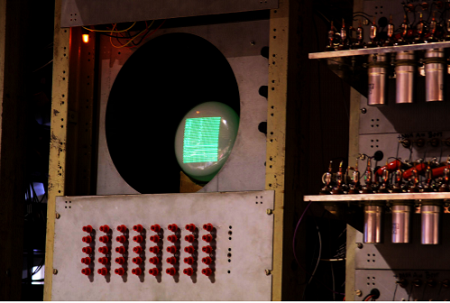
\includegraphics{img/3.PNG}
\end{center}
Il Manchester Baby fu costruito per testare una nuova tecnologia (nuova nel 1948) basata sui tubi catodici: i bit sono memorizzati come punti o linee su uno schermo fluorescente, vengono scritti dirigendo opportunamente un raggio catodico e riletti tramite una griglia metallica che copre lo schermo. Il vantaggio di avere una memoria a tubo catodico è la possibilità di vederne un'immagine rappresentativa con un normale schermo a tubo catodico (come quello dei vecchi televisori). Si osservi una cosa: il software non ha controllo dell'I/O, differenza sostanziale rispetto ad oggi.

\paragraph{Caratteristiche della memoria e registri}
\begin{center}
	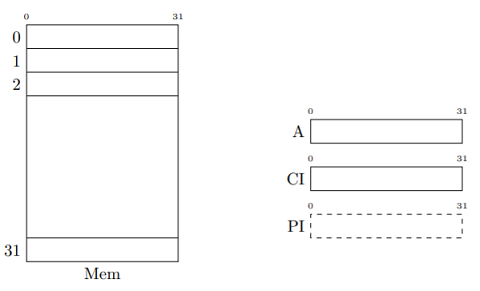
\includegraphics{img/4.PNG}
\end{center}
\begin{itemize}
	\item Abbiamo celle di dimensione a 32 bit. 
	\item Contrariamente a quanto già visto la cifra più significativa sta in posizione 0 e non nell'ultima posizione della cella (ne dobbiamo tenere conto).
	\item Gli indirizzi non sono visibili sullo schermo, ma posti in input con i bottoni del Manchester Baby, Si impostano i bottoni per ottenere una particolare riga e a quel punto la si manipola.
\end{itemize}
Il processore del Manchester Baby presenta tre registri, tutti a 32 bit:
\begin{itemize}
	\item il registro accumulatore A
	\item il registro CI (\emph{Current Instruction})
	\item il registro PI (\emph{Present Instruction})
\end{itemize}

\paragraph{Esecuzione di istruzioni in sequenza} Il processore è una macchina che esegue istruzioni elementari contenute in memoria. Riceve dei numeri e li interpreta come istruzioni, precisamente:
\begin{enumerate}
	\item incrementa CI di 1;
	\item legge dalla memoria la locazione di indirizzo CI e la copia in PI;
	\item esegue l'istruzione contenuta in PI;
	\item se l'istruzione non era di stop, torna al punto 1; altrimenti, accende la lampadina e non fa altro.
\end{enumerate}
Questo ovviamente tenendo conto di eventuali istruzioni di salto (che modifica il contenuto di CI prima che questo venga copiato in PI). Si tenga conto che se l'indirizzo al reset di CI è zero allora la prima istruzione eseguita sarà quella posta all'indirizzo 1. Al di la di queste cose il ragionamento pensato per eseguire istruzioni in sequenza (ed effettuare eventuali salti) è praticamente uguale a quello del processore moderno.

\paragraph{Programmare} Programmare significa porre il contenuto iniziale in memoria in modo tale che la macchina possa lavorare da sola. La cosa non è cambiata: anche oggi programmare significa questo! Il numero posto in una cella, abbiamo già detto, viene considerato dal processore come un'istruzione. Vediamo formato e possibili istruzioni
\begin{center}
	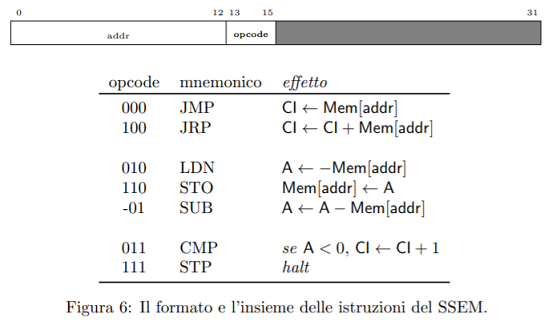
\includegraphics{img/1.PNG}
\end{center}
\begin{itemize}
	\item Formato:
	\begin{itemize}
		\item Dalla posizione 0 alla posizione 12 abbiamo l'indirizzo (\emph{addr}), cioè l'operando.
		\item Dalla posizione 13 alla posizione 15 abbiamo l'OPCODE, cioè l'identificativo dell'istruzione.
		\item I bit rimanenti non presentano contenuto rilevante.
	\end{itemize}
	\item Istruzioni:
	\begin{itemize}
		\item JMP: istruzione di salto non condizionato, pongo in CI il contenuto della cella di memoria Mem[addr]
		\item JRP: jump relativa, aggiorno CI sommando ad esso il contenuto della cella di memoria Mem[addr]
		\item LDN (\emph{LoaD Negative}: aggiorno il registro accumulatore ponendo l'opposto del numero memorizzato in Mem[addr] (rappresentazione in C2)
		\item STO: pongo come contenuto della cella di memoria Mem[addr] il contenuto del registro A.
		\item SUB: sottrazione, sottraggo al contenuto del registro A il contenuto della cella di memoria Mem[addr]. Il risultato della sottrazione è posto nel registro A. Dovendo ridurre all'osso hanno pensato che la sottrazione sia più utile (e che si possa fare un addizione utilizzando la LDN). Per fare l'addizione dobbiamo fare il seguente calcolo
		\[\text{ADDIZIONE }=-(-X-Y)\]
		\item CMP: salto condizionato, se il contenuto del registro accumulatore è minore di 0 viene saltata una istruzione (riduzione all'osso del meccanismo visto in Assembler).
		\item HLT: \emph{halt}, l'esecuzione sequenziale di istruzioni viene fermata e la spia rossa del calcolatore accesa.
	\end{itemize}
\end{itemize}
\paragraph{Esempio di programma che restituisce l'opposto}
\begin{center}
	
\includegraphics{img/2.PNG}
\end{center}
\paragraph{Ulteriore esempio} Nelle appendici è presente la dispensa di Lettieri sul Manchester Baby. Troverete un ulteriore esempio di programmazione col Manchester Baby.
\clearpage
\section{Domanda finale della lezione}
\paragraph{Chi comanda?}
\begin{itemize}
	\item La memoria è una risposta troppo generica.
	\item Il processore non può essere perché esegue gli ordini del software e sa solo ciò che è contenuto nei registri. Non conosce il programma passato, ne tantomeno quello futuro. Non conosce gli effetti complessivi di una set di istruzioni, le esegue singolarmente senza analizzarle da un punto di vista globale.
\end{itemize}
Nel calcolatore chi comanda è il software, è li che risiede l'intelligenza del programma: noi poniamo codice nella memoria, e ciascuna riga indica un'istruzione da eseguire. Questa cosa è l'essenza del \emph{calcolatore programmabile}:  \textbf{modificare ciò che il calcolatore fa senza modificare l'hardware}.
\paragraph{Flusso di controllo} Il software controlla il processore e gli fornisce l'istruzione successiva (e lo fa in modo esplicito nel caso in cui voglia compiere un'istruzione di salto). Con un processore si ha un unico flusso di controllo.
\paragraph{Cosa succede se  il software è composto da più parti?} Supponiamo di avere funzioni di libreria: cosa succede? Si dice che il programma cede il controllo del processore alla funzione di libreria (il processore è come una palla che può rimbalzare da una persona a un'altra). Alla fine la funzione di libreria restituirà il controllo al programma.
	\chapter{Martedì 02/03/2021}
\section{Architettura IBM-compatibile con processore Intel a 64 bit}
Iniziamo a vedere un architettura IBM compatibile con processore Intel a 64 bit. Facciamo alcune premesse.
\begin{itemize}
	\item Dire che una cosa è uscita in un certo anno non significa dire che quella cosa sia stata inventata in quel momento. Certe volte si sente dire che Steve Jobs o Bill Gates hanno inventato il computer, e ciò è una castroneria.
	\item A partire dagli anni 70 si è avuto un processo di miniaturizzazione, che ha portato ad avere calcolatori di dimensione minore, accettabili per l'uso domestico.
\end{itemize}
\paragraph{IBM} Nel 1981 l'IBM decide di entrare nel mercato dei personal computer. Inizia a commercializzare l'IBM PC 5150 e brevetta il personal computer. Il successo è stratosferico, e la concorrenza sbaragliata. 
\begin{center}
	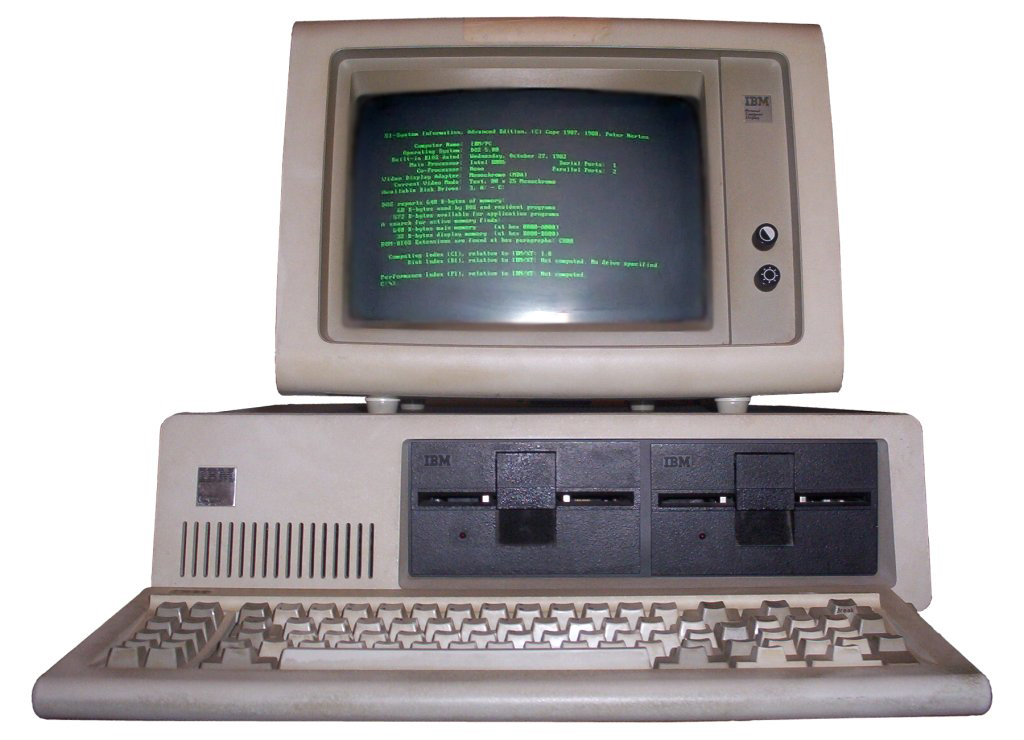
\includegraphics[scale=.25]{img/130.PNG}
\end{center}L'architettura era aperta, quindi fu possibile creare cloni legali detti \emph{IBM compatibili}. Il processore scelto dall'IBM fu l'8088 dell'Intel. 
Si tenga conto che i personal computer, inizialmente, erano molto meno potenti rispetto ai calcolatori per uso professionale. Nel tempo i PC sono stati dotati di tutte le funzionalità che all'epoca erano presenti solo sui calcolatori per uso professionale (interruzioni e protezioni sono cose che non sono state inventate con i PC).
\subsection{Sviluppi del processore INTEL}
\begin{multicols}{2}
	\small
	\begin{itemize}
		\item \textbf{8088 16bit}, con le interruzioni
		\item \textbf{80286 16bit}, con interruzioni e protezione
		\item \textbf{80386 32bit}, con interruzioni, protezione e memoria virtuale
	\end{itemize}
	\normalsize
	\columnbreak
	\begin{center}
		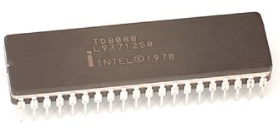
\includegraphics[scale=.75]{img/131.PNG}
	\end{center}
\end{multicols}
\noindent Dopo il terzo modello indicato non si hanno più novità rilevanti. Le novità da allora hanno riguardato soprattutto nuovi set di istruzioni e modifiche interne per velocizzare il processore. Verso la fine degli anni 90 la Intel ha introdotto \emph{Itaniun} per passare da 32 bit a 64 bit. In contemporanea la AMD ha sviluppato un'estensione dell'architettura Intel esistente, nota come \emph{AMD64}. L'Itanium non ha avuto successo e la Intel ha reso i suoi processori compatibili con l'estensione AMD.

\paragraph{Brutture} L'architettura che andremo a vedere è brutta, complicata e irregolare, vittima del suo successo. Il software sviluppato, imponente, è cresciuto negli anni principalmente per motivi di retrocompatibilità. Molte scelte del passato sopravvivono anche oggi in questi processori. 
\subsection[{Confronto col Manchester Baby}]{Confronto col Manchester Baby\footnote{Sono consapevole che questa sezione risulterà un po' antipatica. Riguardatevi modo la struttura del calcolatore). }} Facciamo un confronto con quanto visto ieri.
\begin{itemize}
	\item \textbf{CPU}: il meccanismo di esecuzione delle istruzioni è sostanzialmente simile.
	\begin{itemize}
		\item Prelievo l'istruzione,
		\item eseguo l'istruzione, e
		\item passo all'istruzione successiva.
	\end{itemize}
	La differenza sostanziale sta nella dimensione dell'istruzione: oggi questa è variabile, compresa tra 1 e 18 byte (dipende dai fattori già visti a Reti logiche).
	\item \textbf{Memoria}: vediamo le differenze principali.
	\begin{itemize}
		\item \textbf{Differenza di lana caprina}: memoria di maggiore dimensione
		\item \textbf{Differenze sostanziali}: 
		\begin{itemize}
			\item Nel Manchester Baby si può accedere soltanto a un'intera riga di 32bit (cioè operazioni di lettura e scrittura). Non si poteva intervenire su sottorighe.
			\item Le architetture erano sostanzialmente divise in due categorie: macchine scientifiche con accesso stile Manchester Baby (celle di dimensione ampia), e macchine ad uso commerciale con memorie organizzate a caratteri (byte che avevano dimensione di 5/6 bit). La macchina moderna ingloba entrambe le categorie:
			\begin{itemize}
				\item Ogni singolo byte ha un indirizzo (la dimensione del byte è stata standardizzata, 8 bit). 
				\item La memoria è accessibile non solo a singoli byte, ma anche a multipli del byte (\emph{word, doubleword e quadrupleword}, rispettivamente 16bit, 32bit e 64bit).
			\end{itemize}
		\end{itemize}
	\end{itemize}
	\item \textbf{I/O}:
	\begin{itemize}
		\item L'I/O non è collegato direttamente alla memoria, ma raggiungibile attraverso il bus.
		\item \textbf{Contrariamente al Manchester Baby è necessario del software}: quanto posto nella periferica rimane al suo interno e deve essere recuperato dal software per essere usato (per esempio quando vogliamo conoscere l'ultimo carattere premuto sulla tastiera). L'interfaccia appare al processore come una memoria, come un insieme di registri che possono essere letti e scritti. 
		\begin{center}
			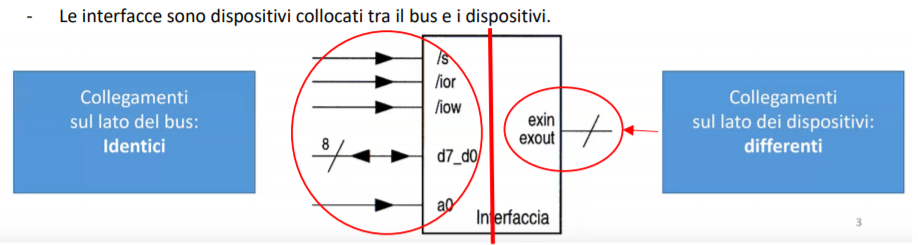
\includegraphics[scale=.75]{img/132.PNG}
		\end{center}
		La differenza importante è che operazioni di lettura e scrittura possono avere effetti collaterali sulle periferiche. 
		
		\begin{itemize}
			\item Gli indirizzi devono essere pensati come qualcosa che appartiene al bus, separato dalla memoria e dall'I/O. Gli indirizzi, tra memoria e I/O, devono essere \underline{UNIVOCI}.
			\item Un'entità attiva, per dialogare, pone sul bus l'indirizzo della cella con cui vuole parlare. Questo indirizzo è visto da tutti coloro che sono collegati al bus, \textbf{non solo da chi reagisce}.
			\item Ognuno degli oggetti collegati al bus deve sapere quali sono i propri indirizzi: in base agli indirizzi ricevuti l'oggetto capisce se deve reagire o meno. Considerando l'univocità è chiaro che in una situazione caratterizzata dalla presenza di tante periferiche solo una di queste risponderà.
		\end{itemize}
		
		\item \textbf{Attenzione}. Storicamente l'architettura prevedeva una distinzione netta tra memoria e I/O (indirizzamenti separati, ripensare alla struttura del calcolatore vista a Reti logiche). Si capiva al volo se la CPU voleva parlare con la memoria o con l'I/O. Nei pc moderni la distinzione è meno netta.
	\end{itemize}
\end{itemize}
\subsubsection{Spazio di memoria} Segue che lo spazio di memoria è una cosa diversa dalla memoria.
\begin{itemize}
	\item \textbf{Lo spazio di memoria è l'insieme di tutto ciò che è indirizzabile}, cioè degli indirizzi che il processore genera quando sta eseguendo un istruzione che ha un operando in memoria, oppure quando sta prelevando un'istruzione.
	\item Tutto ciò che è presente nello spazio di memoria può essere letto con l'istruzione MOV (ovviamente tenendo conto di meccanismi come la protezione).
\end{itemize}
\paragraph{Spazio di memoria comprende lo spazio di I/O?} 
\begin{itemize}
	\item Nell'architettura che vedremo lo spazio di I/O non è parte dello spazio di memoria: la CPU genera un indirizzo nello spazio di I/O quando esegue le istruzioni IN e OUT.
	\item Vedremo che in alcuni casi le periferiche (solitamente quelle "più vecchie") hanno i registri nello spazio di I/O, mentre altre (solitamente quelle più recenti) hanno i loro registri nello spazio di memoria (quindi vi si può accedere con una semplice MOV, basta conoscere l'indirizzo).
\end{itemize} 
\paragraph{Dunque}
\begin{itemize}
	\item La CPU genera un accesso sul bus nello spazio di memoria.
	\item Lo schema prevede che ogni sottoparte dell'oggetto collegato al bus abbia un suo indirizzo diverso: una memoria RAM occupa un intervallo di indirizzi, stessa cosa ogni signola periferica. 
	\item Una volta che l'oggetto ha capito che deve lavorare deve individuare la sottoparte chiamata in causa: prendiamo una periferica, il processore non solo vuole parlare con la periferica, ma vuole anche leggere/scrivere su uno specifico registro.
\end{itemize}
\subsubsection{Introduzione della memoria ROM, utilità della memoria ROM} Altra differenza rispetto al Manchester Baby è la presenza di una memoria ROM, oltre che di una RAM. perché ci serve?
\begin{itemize}
	\item La CPU non fa niente se non c'è del software.
	\item Dobbiamo eseguire il programma bootstrap, cioè fornire del software base. Se io non eseguo questo programma mi ritrovo con una memoria piena di spazzatura, e la CPU interpreta cose casuali come istruzioni (se possibile).
	\item Nel Manchester Baby non abbiamo un programma bootstrap, ma non è un problema visto che \textbf{possiamo inserire roba in memoria senza dover avere qualcosa già in memoria}. Nell'architettura moderna tutto è gestito dal software, incluse le periferiche di I/O: se non ho software non ho nè input nè output. Esco da questo ciclo solo introducendo una memoria di sola lettura.
\end{itemize}
\subsubsection{Differenza tra hardware e software} 
\[\boxed{\text{Il software consiste in tutto ciò che è contenuto in memoria, l'hardware è tutto il resto.}}\]
La confusione è lecita: alcune cose fatte in software potrebbero essere fatte in hardware, e viceversa
\clearpage
\subsection{Riflessioni approfondite sulla CPU} 
Abbiamo capito che il suo scopo è eseguire istruzioni in linguaggio macchina. Queste istruzioni possono fare riferimento ad operandi (ricordarsi che l'istruzione base è quella aritmetica, due operandi che producono un risultato da memorizzare da qualche parte).
\begin{verbatim}
	OPCODE source, destination
\end{verbatim}
\paragraph{Dove si trovano gli operandi?}
\begin{enumerate}
	\item In un registro,
	\item direttamente nell'istruzione (\emph{operando immediato}, costante), o
	\item nello spazio di memoria (ricordiamoci, spazio di memoria adesso è una cosa decisamente più generica).
\end{enumerate}
Per facilitare il parsing l'operando costante inizia col dollaro, mentre il registro con la percentuale. In tutti gli altri casi si ha un operando immediato. Ricordiamoci la regola fondamentale: tutto ciò che ha a che fare con una istruzione deve stare nel processore. Pensiamo al calcolatore a 32 bit visto a Reti logiche: nella fase di fetch tutto ciò che non è presente nel processore viene portato al suo interno.

\subsubsection{Spazio di memoria e regole di indirizzamento (CISC)}
Lo spazio di memoria è la cosa più complessa. L'architettura del processore è detta CISC (\emph{Complex Instruction Set Computer}): il set delle istruzioni è complesso, nel senso che una singola istruzione può fare tante cose\footnote{\textbf{Definizione della Wikipedia inglese}. A complex instruction set computer is a computer in which single instructions can execute several low-level operations (such as a load from memory, an arithmetic operation, and a memory store) or are capable of multi-step operations or addressing modes within single instructions}. Se dobbiamo generare un indirizzo nello spazio di memoria possiamo chiedere al processore di calcolarlo: le metodiche sono le stesse viste a Reti logiche (si vedano le pagine sulle regole di indirizzamento, riprese dalla dispensa di Reti logiche). Si consideri che Lettieri chiama il \emph{displacement} con un altro nome: \emph{offset}.

\subsubsection{Problema: offset dell'indirizzo a 32 bit} L'offset ha dimensione di 32bit. Si è deciso di non espanderlo a 64bit per evitare un aumento eccessivo della dimensione delle istruzioni (inutile nella maggior parte dei casi). perché la cosa è fastidiosa? Prendiamo la seguente istruzione
\begin{verbatim}
	MOV offset, %RAX
\end{verbatim}
il fatto che l'offset sia a 32bit ci permette di porre come source solo i primi 4GB di memoria. La AMD ha introdotto due modi per aggirare il problema:
\begin{itemize}
	\item l'istruzione MOVABS, l'unica istruzione che ha l'offset a 64bit.
	\begin{verbatim}
		MOVABS offset, %RAX <----- N.B. UNICO REGISTRO UTILIZZABILE
		MOVABS $costante, %RAX
		MOVABS %RAX, offset
	\end{verbatim}
	\item L'indirizzamento con registro base e offset a 32bit con segno.
	\begin{verbatim}
		offset(%RIP)
	\end{verbatim}
	che sostanzialmente equivale a dire 
	\[\text{Indirizzo}=\left|\text{base} \pm \text{offset}\right|_{\text{modulo}_{2^{64}}}\]
	ricordarsi che RIP è un registro a 64bit e che l'offset viene esteso con segno (cioè replicando il bit più significative per il numero necessario di volte). In un certo senso equivale a stabilire il punto di riferimento: da questo punto posto in RIP possiamo leggere 2GB indietro e 2GB avanti (ricordarsi del segno). Si osservi che questo tipo indirizzamento \textbf{già esisteva}, ma è stato reso esplicito per gli operandi. Era già presente nelle istruzioni di salto, introdotte così a Reti logiche:
	\begin{verbatim}
		JMP %EIP +- displacement
	\end{verbatim}
\end{itemize}
\subsubsection{Utilità degli indirizzamenti nelle strutture dati} L'idea centrale è che uno piazza le cose in memoria e accede liberamente, nel modo più semplice possibile. La cosa interessante è che attraverso certi tipi di indirizzamenti posso creare delle strutture dati e calcolare velocemente gli indirizzi delle componenti.
\begin{itemize}
	\item \textbf{Array}: l'array è un insieme di elementi consecutivi, tutti dello stesso tipo. Il dimensionamento di ogni singolo elemento è lo stesso, quindi mi basta indicare il numero di bit di ciascun elemento attraverso la scala e incrementare il registro indice ogni volta.
	\[\text{Indirizzo}=\left|\text{base} \pm \text{indice} \times \text{scala}\right|_{\text{modulo}_{2^{64}}}\]
	\item \textbf{Struttura}: ho una serie di elementi consecutivi, di dimensione diversa tra loro. Ho indirizzi diversi, ma uno scostamento costante rispetto all'indirizzo base. Questo scostamento è posto nella definizione della struttura.
	\item \textbf{Puntatore}: il puntatore equivale all'indirizzamento di tipo indiretto con registro base. bit di ciascun elemento attraverso la scala e incrementare il registro indice ogni volta.
	\[\text{Indirizzo}=\left|\text{base}\right|_{\text{modulo}_{2^{64}}}\]
\end{itemize}
\clearpage 
\subsubsection{Registri} Rispetto a Reti logiche abbiamo più registri, tutti di dimensione maggiore. Sono tutti interni al processore e sono la unità di memorizzazione più veloce che ci sia. Un registro può essere letto e scritto in un ciclo di clock, cosa assolutamente impossibile con una RAM (la lettura/scrittura può richiedere centinaia di clock). 
\begin{center}
	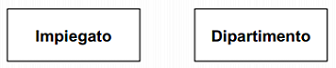
\includegraphics{img/5.PNG}
\end{center}
\begin{itemize}
	\item I registri già esistenti nell'architettura a 32bit sono stati mantenuti.
	\item Il registro dei flag è stato esteso a 64bit, ma non contiene nuovi flag. Anche l'instruction pointer è stato esteso a 64 bit.
	\item I registri rimanenti sono stati estesi e contengono la loro vecchia versione a 32bit: i nomi per richiamarle \underline{sono esattamente gli stessi}!
	\item La AMD ha uniformato gli accessi, nel senso che nei rimanenti registri a 64bit troviamo SEMPRE la versione a 16bit e 8bit (cosa che non era valida per alcuni registri, ripensare a Reti logiche). 
	\item Resta una irregolarità: solo i registri A, B, C, D sono accessibili anche nella parte più significativa dei primi 16bit (AH, BH, CH, DH), gli altri sono accessibili solo nella parte meno significativa.
\end{itemize}
A differenza del manchester baby abbiamo (cose già viste a Reti):
\begin{itemize}
	\item istruzioni che alterano in modo implicito il registro stackpointer (per esempio la chiamata di funzione, tutto ciò che è legato alla pila);
	\item istruzioni che alterano il registro dei flag settandoli (per esempio STD e CLD);
	\item istruzioni che verificano se sono presenti specifiche configurazioni di flag e decidono, conseguentemente, se fare salto o meno (JMP condizionate, il Manchester Baby prevedeva un JMP condizionata molto primitiva\footnote{Verificare se il numero posto nel registro accumulatore è positivo o negativo, dunque fare un eventuale salto DI UNA SOLA ISTRUZIONE.}).
\end{itemize}
	\chapter{Giovedì 04/03/2021 e Venerdì 05/03/2021}
%\section{Spazio di memoria, dimensionamento della memoria, formato degli indirizzi}
\section{Unità di misura della memoria} Dato un numero di bit, vogliamo indicare la dimensione dell'area di memoria con le apposite unità di misura. Osserviamo le potenze
\begin{align*}2^2=4&&2^3=8&&2^4=16&&2^5=32&&2^6=64&&2^7=128&&2^8=256&&2^9=512&&\boxed{2^{10}=1024}\end{align*}
A questo punto i dubbi ci vengono. Noi informatici abbiamo sempre abusato di queste lettere....
\begin{align*}
	2^{10}\simeq 1000 &\longrightarrow K&2^{20}\simeq 1000000 &\longrightarrow M\\
	2^{30}\simeq \dots &\longrightarrow G&2^{40}\simeq \dots &\longrightarrow T
\end{align*}
Cerchiamo di risolvere la confusione con la seguente tabella\begin{center}\begin{tabular}{ |l|c|l|l|c|l|} \hline\multicolumn{3}{|c|}{\textbf{Misure binarie}} & \multicolumn{3}{c|}{\textbf{Misure decimali}} \\\hline\textbf{Nome} & \textbf{Fattore} & \textbf{Valore in byte} & \textbf{Nome} & \textbf{Fattore} & \textbf{Valore in byte}\\\hline
		kibibyte (KiB) & $2^{10}$ & 1,024 & kilobyte (KB) & ${10}^3$ & 1,000\\ 
		\hline
		mebibyte (MiB) & $2^{20}$ & 1,048,576 & megabyte (MB) & ${10}^6$  & 1,000,000\\ 
		\hline
		gibibyte (GiB) & $2^{30}$ & 1,073,741,824 & gigabyte (GB) & ${10}^9$  & 1,000,000,000\\ 
		\hline
		tebibyte (TiB) & $2^{40}$ & 1,099,511,627,776 & terabyte (TB) & ${10}^{12}$  & 1,000,000,000,000\\ 
		\hline
	\end{tabular}
\end{center}

\noindent Abbiamo introdotto delle nuove unità di misura. Quelle "tradizionali" a cui siamo abituati sono \emph{misure decimali}, mentre quelle nuove sono \emph{misure binarie}. 
\begin{align*} 
	1\,\text{KB}&=1000\,\text{byte}&1\,\text{KiB}&=1024\,\text{byte}&\Delta&=24\,\text{byte}\\
	2\,\text{KB}&=2*1000=2000\,\text{byte}&2\,\text{KiB}&=2*1024=2048\,\text{byte}&\Delta&=48\,\text{byte}\\
	3\,\text{KB}&=3*1000=3000\,\text{byte}&3\,\text{KiB}&=3*1024=3072\,\text{byte}&\Delta&=72\,\text{byte}\\
	&=\dots&&=\dots&&=\dots\\
	N\,\text{KB}&=N*1000=N*{10}^3&N\,\text{KiB}&=N*1024=N*{10}^3+N*24&\Delta&=N*24\,\text{byte}
\end{align*}
Risulta facile capire che più le dimensioni aumentano più le misure binarie si discostano da quelle decimali.

\paragraph{Quanto spazio ho con 48 bit?} $2^{48}=2^{40} \cdot 2^{8}= 256\,\text{TiB}$
\paragraph{Quanto spazio ho con 57 bit?} $2^{57}=2^{50} \cdot 2^{7}= 128\,\text{PiB}$

\section{Spazio di memoria non completo e "buco"} Lo spazio di memoria non è completo: non tutti i 64bit che compongono un indirizzo sono implementati. La AMD si è riservata di poterne aggiungere in futuro. Lo ha già fatto: i primi processori avevano solo 48 bit significativi, adesso i bit significativi sono 57. Bit in più comportano complicazioni in più, soprattutto costo maggiore nell'utilizzo.
\paragraph{Formato degli indirizzi} \[\boxed{\text{I bit non utilizzati devono essere uguali al bit più significativo tra quelli utilizzati.}}\]Gli indirizzi che rispettano il formato sono detti in \textbf{forma canonica}. All'interno del processore esiste un meccanismo di protezione che impedisce al processore di andare avanti se l'indirizzo posto non rispetta il formato. La AMD ha adottato questo meccanismo remore dell'esperienza della IBM. Questa, quando ha cercato di implementare indirizzi più grandi, ha avuto problemi: molti programmi hanno smesso di funzionare perché utilizzavano i fili di indirizzo non implementati per altri scopi.

\paragraph{Conseguenza} All'interno dello spazio di memoria abbiamo una sorta di buco, che va dall'ultimo indirizzo avente tutti e 7 i bit più significativi uguali a $0$ al primo indirizzo avente tutti e 7 i bit più significativi uguali ad $1$.

\section{Esempio di programma Assembler}
\paragraph{Esami su Linux} Gli esami saranno svolti su macchina virtuale con Debian. Non è necessario avere grande dimestichezza verso questo sistema operativo.
\paragraph{Funzionamento}
\begin{itemize}
	\item Produciamo un file editor.s
	\item L'assemblatore produce, a partire dal file precedente, un file oggetto .o. I file oggetto sono semplici dati, nulla di eseguibile. 
	\item Il collegatore unisce questo file oggetto con altri files oggetto (librerie) e crea un eseguibile. 
\end{itemize}
Contrariamente al Manchester Baby \textbf{stiamo creando programmi utilizzando altri programmi}. Non è necessario che i files oggetto siano presenti sul dispositivo dove avvieremo l'eseguibile: quando acquistiamo un programma abbiamo solo ciò che serve per eseguire il programma, non gli elementi utilizzati per creare il programma.
\paragraph{Come creiamo programmi in una macchina nuova che non ha assemblatore?} Creiamo l'assemblatore e il collegatore su una macchina già esistente: il risultato gira sulla macchina vecchia, ma funziona anche sulla macchina nuova. Otteniamo l'eseguibile sulla macchina vecchia e lo poniamo nella macchina nuova. 
\paragraph{In che linguaggio è scritto il compilatore per il C?} In C. Come è possibile? 
\begin{itemize}
	\item I compilatori moderni sono compilati da versioni precedenti.
	\item La prima versione del compilatori in C è scritta in un altro linguaggio.
	\item I primi compilatori, successivamente, sono stati scritti in linguaggio assembler.
	\item I primi assemblatori sono stati scritti in linguaggio macchina.
\end{itemize}
\paragraph{Assemblatore} L'assemblatore traduce dal linguaggio assembler al linguaggio macchina. Precisamente, lo vediamo dal nome, l'assemblatore assembla il contenuto della memoria (programmare significa indicare il contenuto iniziale della memoria). Fa ciò che noi abbiamo fatto a mano per scrivere un programma nel Manchester Baby.
\paragraph{perché separare assemblatore e collegatore?} Conviene scrivere questi pezzi di memoria senza decidere dall'inizio dove dovranno essere caricati. Scrive le cose, ma rimanda la decisione: questo perché vuole scrivere tanti pezzi (quando scrive un pezzo non sa riguardo gli altri). 

\paragraph{Codice}
\small
\begin{verbatim}
	.data
	num1:
	.quad 0x1122334455667788
	num2:
	.quad 0x9900aabbccddeeff
	risu:
	.quad -1
	
	.text
	.global _start
	_start:
	movabs num1, %rax
	mov %rax, %rbx
	movabs num2, %rax
	add %rbx, %rax
	movabs %rax, risu
	
	# uscita
	mov $0, %rbx   
	mov $1, %rax
	int $0x80
\end{verbatim}
\normalsize
\paragraph{Raggiungiamo il terminale}
\begin{center}
	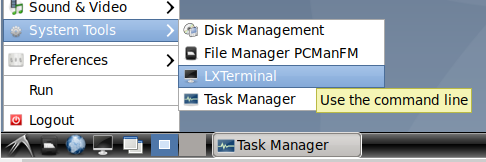
\includegraphics{img/138.PNG}
\end{center}
\paragraph{Comandi eseguiti} In una riga pongo prima il comando, e poi gli argomenti
\begin{itemize}
	\item \begin{verbatim}ls\end{verbatim}
	carico la lista dei files presenti nella directory
	\begin{center}
		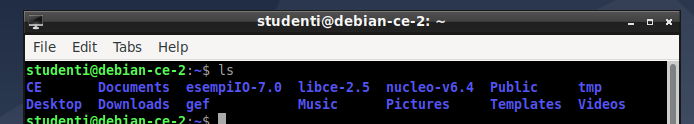
\includegraphics[scale=.8]{img/135.PNG}
	\end{center}
	se non sono presenti files/cartelle non restituisce nulla.
	\item \begin{verbatim}cd nome_cartella\end{verbatim}
	accedo a una directory
	\begin{center}
		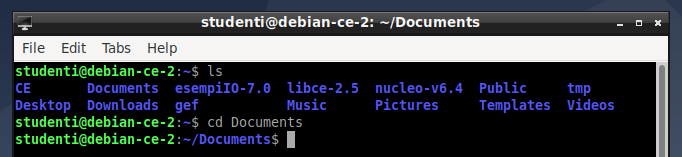
\includegraphics[scale=.8]{img/136.PNG}
	\end{center}
	Nel caso in cui la directory non esista viene restituito l'errore \emph{No such file or directory}. Per tornare indietro di una directory basta porre due punti come nome della cartella
	\begin{center}
		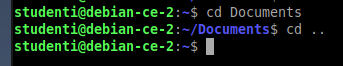
\includegraphics[scale=.9]{img/137.PNG}
	\end{center}
	\item \begin{verbatim}mkdir nome_cartella\end{verbatim}
	creo una cartella col nome indicato.
	\item \begin{verbatim}vi sum.s\end{verbatim}
	carico l'editor di modifica per il file \emph{sum.s}. 
	\begin{center}
		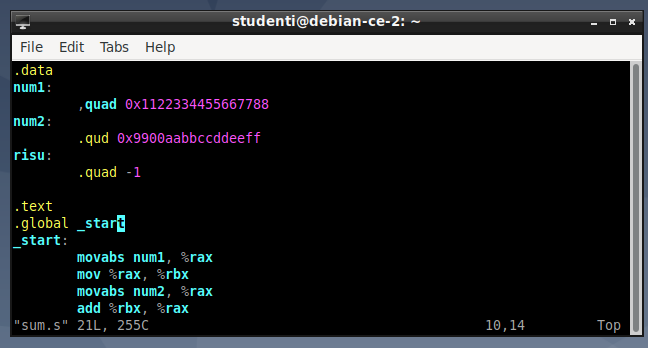
\includegraphics[scale=.8]{img/139.PNG}
	\end{center}Se il file esiste viene caricato l'editor di modifica per quel file, se non esiste viene caricato l'editor lo stesso e in caso di salvataggio viene creato. Si tenga conto che al caricamento dell'editor entriamo in modalità comando.
	\begin{itemize}
		\item Per entrare in modalità modifica digitare la seguente lettera
		\begin{verbatim}i\end{verbatim}
		che permette di iniziare la modifica a partire dal carattere dove si trova il cursore del terminale (altre lettere permettono di entrare in modalità modifica, la differenza sta nel punto da dove inizieremo a modificare).
		\item Per ritornare alla modalità comando basta utilizzare il tasto \emph{ESC}.
		\item Per annullare modifiche precedenti digitare la seguente lettera
		\begin{verbatim}u\end{verbatim}
		\item Per chiudere l'editor e salvare le modifiche fatte utilizzare il seguente comando
		\begin{verbatim}:wq\end{verbatim}
		se invece non vogliamo salvare le modifiche
		\begin{verbatim}:q\end{verbatim}
	\end{itemize}
	\item \begin{verbatim}as -o sum.o sum.s\end{verbatim}
	indico che voglio assemblare il programma. Tradizione UNIX è l'assenza di messaggi se tutto va bene. Indico col secondo parametro il nome da dare all'output (\emph{sum.o}), mentre col terzo indico il file Assembler che voglio assemblare (\emph{sum.s}). 
	\item \begin{verbatim}objdump -d sum.o\end{verbatim}
	esamino il contenuto del file oggetto indicato. Con l'opzione d chiedo il \emph{disassembly}, cioè chiedo di rigenerare il file assembler originario partendo dal binario. \begin{center}
		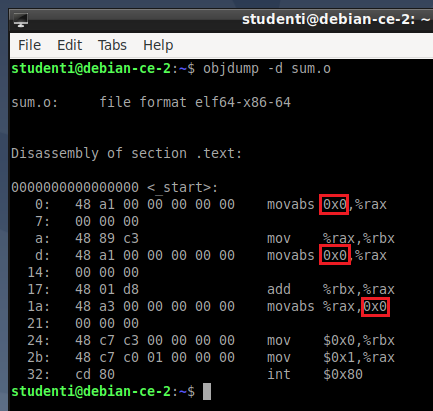
\includegraphics{img/140.PNG}
	\end{center}
	\begin{itemize}
		\item Il formato del file disassemblato è: \emph{file format elf64-x86-6}
		\item Si osservi che l'assemblatore non sa dove stanno \emph{$\_$start}, \emph{num1}, \emph{num2} e \emph{risu}.
		\begin{itemize}
			\item Nella prima \emph{movabs} non sappiamo dove finirà \emph{num1} (e non può fare ipotesi sull'offset, visto che le parti data e le parti text saranno unificate in presenza di più files). L'istruzione è identificata dal byte \emph{a1}, che rappresenta l'istruzione e il passaggio da un indirizzo al registro RAX. Sono riservati 8 byte per l'indirizzo.
			\item La prima \emph{mov} ha solo operandi registro, è molto più compatta. La codifica identifica la \emph{mov} e il passaggio da registro RAX a registro RBX (\emph{89 c3}).
			\item Il numero 48, posto all'inizio di alcune istruzioni, è il prefisso introdotto dalla AMD per le istruzioni che devono usare operandi a 64 bit (codice riciclato, nell'architettura a 32 bit apparteneva alle istruzioni INC).
			
		\end{itemize}
		
	\end{itemize}
	
	\item \begin{verbatim}nm -n sum.o\end{verbatim}
	lista degli offset assegnati ai vari simboli.\begin{center}
		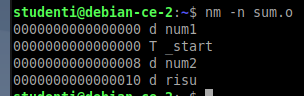
\includegraphics{img/141.PNG}
	\end{center}
	abbiamo le etichette utilizzate in \emph{.data} e in \emph{.text}.
	\item \begin{verbatim}ld -o sum sum.o\end{verbatim}
	collegatore, indico come argomenti i files oggetto da collegare. Viene generato il file eseguibile.
	\item \begin{verbatim}./sum\end{verbatim}
	indico il nome dell'eseguibile per eseguire il programma. In questo caso non viene mostrato nulla, visto che il programma effettua solo spostamenti di memoria.
	\item \begin{verbatim}objdump -d sum\end{verbatim}
	richiedo nuovamente il \emph{disassembly}. \begin{center}
		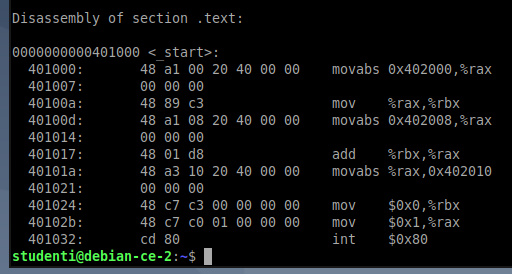
\includegraphics{img/142.PNG}
	\end{center}Otteniamo la stessa cosa di prima, ma vediamo che gli indirizzi dei dati sono definiti. Domanda che sorge spontanea: l'eseguibile è un file oggetto? Il file oggetto visto prima e l'eseguibile hanno lo stesso formato (\emph{file format elf64-x86-6}). 
	\begin{itemize}
		\item L'OPCODE occupa al più due byte.
		\item In presenza di indirizzi e costanti aumenta la dimensione dell'istruzione. Si ha minore occupazione di memoria coi registri.
		\item Attenzione al \emph{little-endian}.
	\end{itemize}
\end{itemize}


\paragraph{Ragioniamo sul programma}
\begin{itemize}
	\item Il programma ha lo scopo di sommare due numeri \emph{quad}. 
	\item Si osservino i passaggi che facciamo con l'istruzione \emph{movabs}, necessari per evitare probabili troncamenti dell'indirizzo a causa dell'\emph{offset} a 32 bit (spazio insufficiente per contenere l'intero indirizzo, se succede il programma inchioda e segnala errore). La cosa dipende da dove sarà collocato in memoria il nostro programma: non lo possiamo sapere a priori, dunque conviene prevenire. 
	\item La movabs viene eseguita più volte poichè l'unico registro destinatario possibile è RAX.
	\item Il collegatore vede solo le etichette .global 
	\begin{verbatim}
		.global _start
	\end{verbatim}In questo caso la utilizzo per dichiarare l'\emph{entry point} del mio programma.
	\item In .data inizializzo i byte che conterranno i miei dati.  
	\begin{verbatim}
		.data
		num1:
		.quad 0x1122334455667788
		num2:
		.quad 0x9900aabbccddeeff
		risu:
		.quad -1
	\end{verbatim}
	Possiamo inizializzare \emph{byte} (8 bit, 1 byte), \emph{word} (16 bit), \emph{long} (32 bit) e \emph{quad} (64 bit). Si consideri che le etichette non occupano spazio e ci permettono di dare nomi ad aree che vedranno associato un indirizzo solo dopo. 
	\item \textbf{Cosa succede se non definisco il valore iniziale dell'insieme di byte introdotto con la direttiva?} Non viene allocato lo spazio! 
	\item \textbf{Non è importante ottimizzare il programma}: non vogliamo diventare programmatori di Assembler. Il compilatore è molto più bravo di noi in questo.
	
	\item \textbf{Sintassi nuova a 64bit}. Riprendiamo la seguente cosa
	\begin{verbatim}
		num1(%rip)
	\end{verbatim}
	L'assemblatore prende questa cosa come l'ordine di calcolare l'offset tra num1 e rip, cioè la differenza. Questa "scappatoia" permette di risolvere il problema del troncamento dell'indirizzo per spazio insufficiente. Il disassemblatore, se abbiamo utilizzato il collegatore, ci restituisce l'indirizzo. Si osservi che in instruzioni diverse l'offset è diverso. Il fatto che non siamo noi a calcolare l'offset è sicuramente una semplificazione. Se riprendiamo gli esempi di indirizzamento di Reti logiche ci ricordiamo che in quei casi dobbiamo indicare noi lo scostamento. Nel caso spiegato ora no.
	
	\item \textbf{Accesso ad aree di memoria}. L'idea base è che io possa accedere esclusivamente alle cose che ho dichiarato. Questa cosa è assolutamente falsa: io posso scrivere dove mi pare, tenendo conto di alcuni limiti. Il kernel, se accediamo ad aree di memoria dove non abbiamo permessi, ci segnala errore di \emph{Segmentation Fault}. Osserviamo lo spazio allocato per il nostro programma: se io accedo a 402000 (dove c'è num1) non avrò problemi. Posso accedere senza problemi fino all'indirizzo 402ff0 (se eseguo un'operazione di MOV non ho problemi). Non appena mi sposto di un solo byte mi viene nuovamente segnalato segmentation fault.
	\item \textbf{Cosa succede se scrivo..?}
	\begin{verbatim}
		mov %rax, num1+16
	\end{verbatim}
	Scrivo su risu. Chi calcola questa espressione? L'assemblatore o il collegatore (in questo caso il collegatore, num1 non è conosciuto dall'assemblatore)! Abbiamo un'espressione costante.
	Si osservi che l'assemblatore sa fare solo espressioni semplici.
\end{itemize}



\subsection{Debugger} Utilizzeremo lo GNU debugger, che possiamo chiamare col seguente comando
\begin{verbatim}
	gdb sum
\end{verbatim}
dove \emph{sum} è il nome dell'eseguibile.
\begin{center}
	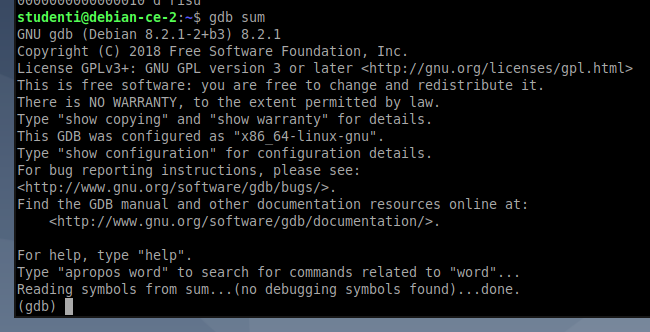
\includegraphics{img/143.PNG}
\end{center}
Il debugger è lo stesso visto a Reti logiche! Purtroppo è abbastanza spartano... Possiamo renderlo un po' più piacevole introducendo l'estensione \emph{gef} col seguente comando
\begin{verbatim}
	source ~/gef/gef.py
\end{verbatim}
Il programma non parte finchè non eseguiamo il comando \emph{start}. Il programma parte e subito si ferma, restituendo il controllo al debugger.
\begin{center}
	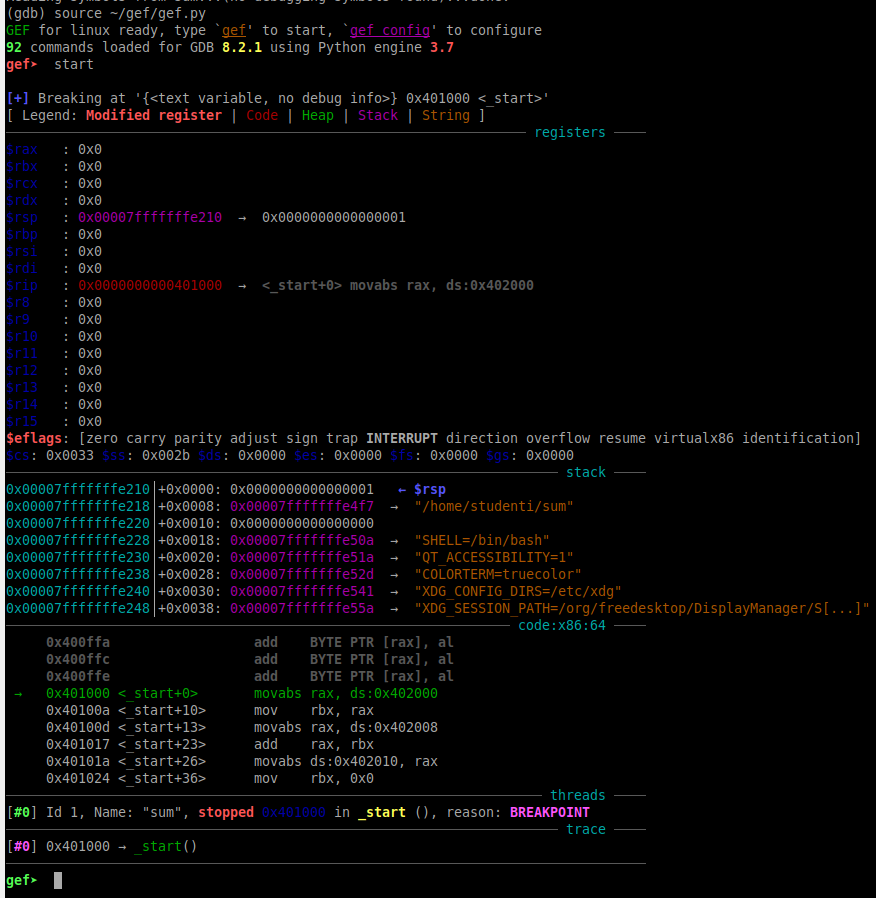
\includegraphics[scale=.9]{img/144.PNG}
\end{center}
L'estensione gef ci mostra, ogni volta che si ferma il debugger:
\begin{itemize}
	\item la lista dei registri con relativo contenuto (vengono evidenziati i registri che sono cambiati di valore rispetto alla "fermata" precedente);
	\item tra i registri quello dei flag (nomi dei flag, evidenziati se il valore è 1);
	\item la pila;
	\item il disassemblato.
\end{itemize}
Vediamo alcune azioni che potrebbero tornarci comode:
\begin{itemize}
	\item \textbf{Disassemblato in formato Intel}: il disassemblato di default (quello in foto) è in sintassi Intel, possiamo impostare la sintassi a cui siamo abituati con i seguenti due comandi
	\begin{verbatim}
		set disassembly-flavor att <----- imposto la sintassi a cui siamo abituati
		context <---- ricarico il contenuto
	\end{verbatim}
	\begin{center}
		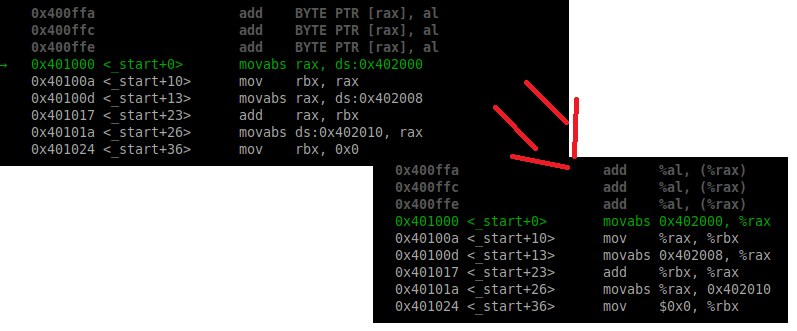
\includegraphics[scale=.9]{img/145.PNG}
	\end{center}
	\item \textbf{Configurazione dell'estensione gef}: il seguente comando
	\begin{verbatim}
		gef config
	\end{verbatim}
	mi permette di caricare la lista delle impostazioni dell'estensione gef.
	\begin{center}
		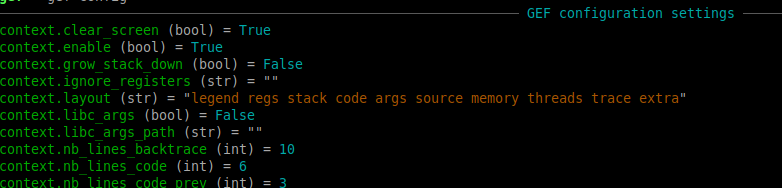
\includegraphics{img/146.PNG}
	\end{center}
	\item \textbf{Modifica di impostazioni dell'estensione gef}: modifichiamo un'impostazione, precisamente la context.layout che indica cosa deve apparirci ogni volta che eseguiamo la context
	\begin{verbatim}
		gef config context.layout "regs code memory"
		context
	\end{verbatim}
	in questo modo abbiamo rimosso la pila (visibile per default, per il momento non ci serve). Mostriamo solo registri, codice e memoria.
	\begin{center}
		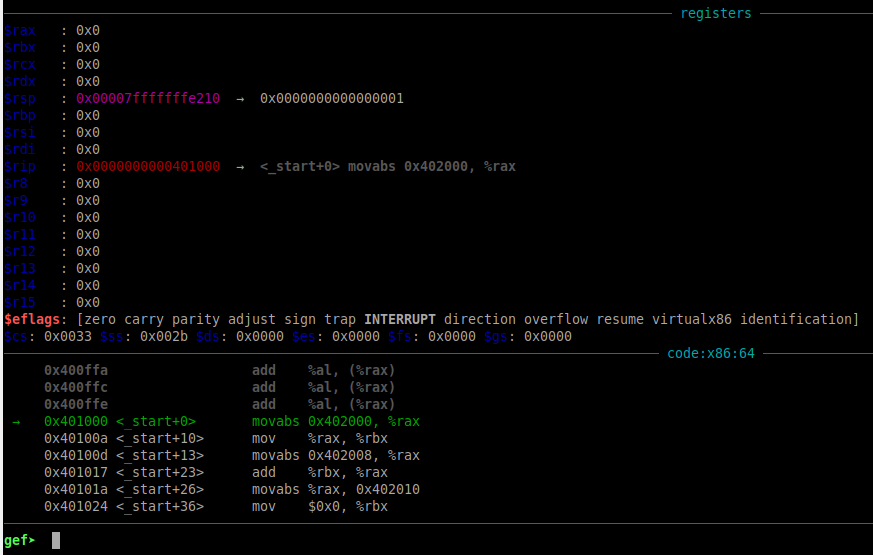
\includegraphics[scale=.9]{img/147.PNG}
	\end{center}
	\item \textbf{Contenuto della memoria a partire da un certo indirizzo nella schermata}: col seguente comando chiediamo di mostrare, a partire dall'indirizzo num1, tre qword
	\begin{verbatim}
		memory watch &num1 3 qword
		context
	\end{verbatim}
	\begin{center}
		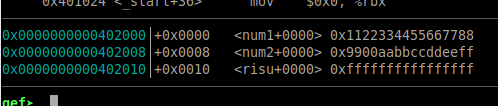
\includegraphics[scale=.9]{img/148.PNG}
	\end{center}
	\item \textbf{Esecuzione di una singola istruzione}: col seguente comando 
	il debugger cede il controllo al programma per eseguire una singola istruzione.
	\begin{verbatim}
		si
	\end{verbatim} 
	\item \textbf{Uscita dal debugger}. Ricordiamo il comando per uscire dal debugger
	\begin{verbatim}
		quit
	\end{verbatim}
\end{itemize}

\section{Indirizzi}
Abbiamo già detto che il processore lavora con indirizzi, e che ogni cosa deve essere identificata mediante un indirizzo.
\begin{itemize}
	\item \textbf{Prima cosa necessaria è avere dimestichezza con i numeri esadecimali}: sono comodi, una cifra esadecimale mi rappresenta quattro cifre binarie.
	%\item Certe volte servono anche i numeri ottali: una cifra ottale mi rappresenta tre cifre binarie. Le proprietà sono le stesse dei numeri esadecimali (l'unica differenza è il considerare terne invece di quaterne). La rappresentazione era utilizzata soprattutto in passato, quando i byte non esistevano ancora e i caratteri erano rappresentati su 6 bit.
	\item Gli indirizzi \emph{vanno pensati come circolari}: ripensare all'operatore modulo di Reti logiche.
	\[|11111111+00000001|_{2^8}=00000000\]
	\item Per rappresentare un indirizzo in C utilizziamo l'\emph{\textbf{unsigned long}}. Attenzione alle direttive:
	\begin{itemize}
		\item in caso di overflow di un \emph{unsigned long} ripartiamo da zero (cosa pensata proprio per gli indirizzi);
		\item in caso di overflow di un \emph{long} sostanzialmente \emph{fa quello che vuole}, si ottiene un \emph{undefined value}.
	\end{itemize}
	\item Il compilatore del C può assumere, per motivi di efficienza, che la condizione non accada mai. Prendiamo il seguente esempio
	\begin{verbatim}
		long x;
		if(x+1 < x)
		...
	\end{verbatim}
	il compilatore ignora completamente la condizione, visto che non sarà mai vera. \textbf{Non avverrà la stessa cosa in presenza di un \emph{unsigned long}}: in quel caso la condizione ha senso e permette di verificare se c'è stato overflow.
\end{itemize}
\subsection{\emph{Offset} (o scostamento)}
\begin{itemize}
	\item L'\emph{offset} consiste nella distanza tra due indirizzi $x$ ed $y$. 
	\item Lo scostamento, precisamente, rappresenta il numero di byte che dobbiamo saltare per passare dall'indirizzo $x$ all'indirizzo $y$. 
	\item La cosa vale con $x<y$, ma anche con $x>y$ (cioè l'offset può essere anche negativo). Vale anche quando abbiamo l'overflow, e quindi il modulo riparte da zero (circolarità dell'operatore modulo).
	\item \textbf{Attenzione} al dimensionamento dell'area dove poniamo l'offset. Se è inferiore alla dimensione degli indirizzi potrebbero emergere problemi.
\end{itemize}
\clearpage 

\subsection{Intervalli (\emph{range})} 
Un intervallo è una sequenza di indirizzi.
\paragraph{Convenzione}
Per convenzione gli intervalli presentano la seguente forma
\[[x,y)=\{z|x \leq z < y\}\,\,\,\,\,\,\,\,\text{con $x \geq y$}\]
Questo ci permette di combinare facilmente due intervalli consecutivi. Per semplicità evitiamo di considerare intervalli che attraversano l'ultimo indirizzo rappresentabile e ripartono da zero (che avrebbero $y<x$). L'insieme $[x,y)$ è vuoto se $y\leq x$.
\paragraph{Grandezza dell'intervallo} La grandezza dell'intervallo è esattamente $y-x$.
\paragraph{Base dell'intervallo} $x$ è detta \emph{base dell'intervallo}. Il suo indirizzo è l'indirizzo dell'intervallo.
\subsubsection{Divisione dello spazio di memoria in parti uguali}
Molto spesso conviene immaginare lo spazio di memoria diviso in parti uguali, ciascuna di dimensione di una potenza di due. 
I punti in cui si passa da un intervallo a un altro sono detti \emph{confini}. L'area compresa tra due confini non ha un nome in letteratura, noi la chiameremo \emph{regione naturale}.
Un indirizzo che si trova al confine si riconosce in maniera immediata:
\begin{center}
	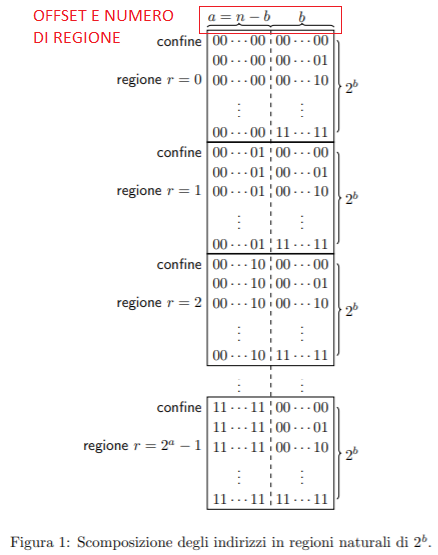
\includegraphics{img/6.PNG}
\end{center}
Osserviamo la struttura dell'indirizzo di base e la struttura dell'ultimo indirizzo di un intervallo. Dati $n$ bit di un indirizzo avrò:
\begin{itemize}
	\item i $b$ bit meno significativi come \textbf{offset} (precisamente l'offset rispetto all'indirizzo di base del relativo intervallo), e
	\item gli $n-b$ bit più significativi come \textbf{numero di regione}.
\end{itemize}
\begin{framed}
	\noindent \textbf{Come pongo questi numeri in due variabili C++?}
	\begin{verbatim}
		unsigned long x;
		
		unsigned long nr = x >> b;
		unsigned long off = x & ((1 << b) - 1);
	\end{verbatim}
	\begin{itemize}
		\item \textbf{Numero di regione}: traslo a destra $b$ volte. Non posso usare una maschera perché otterrei il numero di regione naturale moltiplicato per $2^b$.
		\item \textbf{offset}: utilizzo l'operatore AND e una maschera che mi lascia solo i $b$ bit meno significativi. L'operazione mi permette di ottenere $2^b-1$.
	\end{itemize}
\end{framed}
\paragraph{Intervallo che inizia in una regione e finisce in un'altra} Come trovo l'ultima regione toccata dall'intervallo $[x,y)$ ? 
\begin{itemize}
	\item Per prima cosa devo controllare che l'intervallo non sia vuoto, per esempio $[x,x)$, 
	\item se non lo è mi basta prendere il numero di regione di $y$.
\end{itemize}
\paragraph{perché ci servono queste spiegazioni?} Parleremo di memoria RAM e periferiche che occupano porzioni di indirizzi, appunto \emph{intervalli}. Lavoreremo (con una singola istruzione) su oggetti di un byte, due, quattro, otto byte.

\paragraph{Oggetto allineato in memoria} Un oggetto si dice \emph{allineato} a qualcosa se il suo indirizzo è multiplo di una qualche potenza di due, cioè se l'indirizzo si trova a confine di una qualche regione naturale. Vediamo delle espressioni frequenti:
\begin{itemize}
	\item Oggetto allineato a $2^b$
	\item Oggetto allineato a $Y$ (cioè un oggetto tale che $\dim Y = 2^b$)
	\item Oggetto allineato naturalmente (cioè l'oggetto è allineato alla sua dimensione, $\dim 2^b$).
\end{itemize}
	
\chapter{Lunedì 08/03/2021}
\section{Riprendiamo sullo spazio di memoria}
La differenza principale rispetto al Manchester Baby è il fatto che nelle memorie moderne è possibile accedere sia al byte che a multipli del byte. Questo comporta due questioni.
\subsection{\emph{endiannes}}
Abbiamo visto nel Manchester Baby una disposizione "strana" dei bit. Finché lavoriamo sulle singole righe, come nel Manchester Baby, non è un problema. Se iniziamo a lavorare su multipli e sottomultipli (come in tutte le architetture moderne) diventa necessario conoscere nel dettaglio come sono disposti i vari byte. Si distinguono\footnote{Satira derivante dai viaggi di Gulliver, il nome è diventato popolare in letteratura.} 
\begin{itemize}
	\item \emph{little-endian}: il byte meno significativo si trova all'indirizzo più piccolo;
	\item \emph{big-endian}: il byte più significativo si trova all'indirizzo più piccolo.
\end{itemize}
\paragraph{Rappresentazione dell'indirizzo $0x1A2B3C4D5E6F7080$}
\begin{center}
	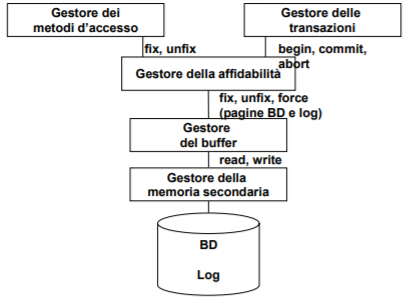
\includegraphics[scale=0.60]{img/134.PNG}
\end{center}
\paragraph{Quando nasce il problema "si fa in un modo o in un altro"?} In due occasioni:
\begin{itemize} 
	\item nascita delle reti, quindi necessità di far comunicare dispositivi con approccio diverso;
	\item nascita dell'esigenza di portare un sistema operativo da un'architettura a un'altra.
\end{itemize}
I sistemi operativi nascono normalmente per un'architettura, e sono scritti in Assembler (che è \emph{processor-specific}). UNIX è uno dei primi sistemi operativi scritti in C, rendeva possibile il passaggio da un'architettura a un'altra.  
\paragraph{Vincitori di questa guerra santa?} 
\begin{itemize}
	\item L'architettura Intel è realizzata con approccio \emph{litte-endian} (quindi noi dobbiamo ragionare così). Tutte le macchine moderne seguono questo approccio, tramite alcuni calculatori IBM professionali.
	\begin{center}
		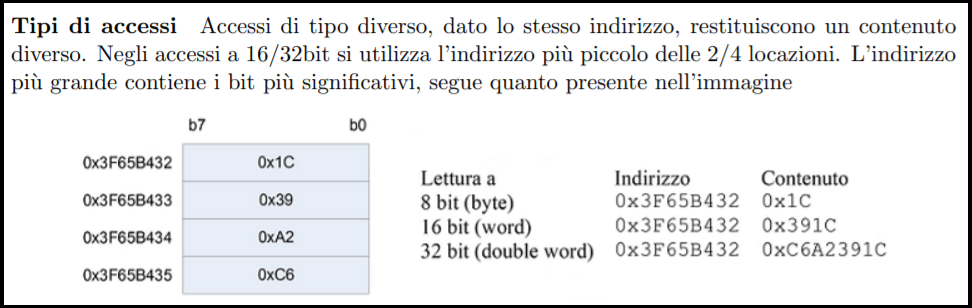
\includegraphics[scale=.65]{img/133.PNG}
	\end{center}
	\item Sulla rete ha vinto \emph{big-endian}.  Segue che un processore Intel dovrà scambiare i byte prima di inviarli.
\end{itemize}

\subsection{\emph{parallelismo}}
Quando il processore legge una parola di 8 byte il nostro interesse è leggerli tutti insieme, quindi \emph{in parallelo}. Dobbiamo organizzare la memoria in modo tale che ciò sia possibile.  
\begin{verbatim}
	MOV %AL, 1000
	MOV %AX, 1000
	MOV %EAX, 1000
	MOV %RAX, 1000
\end{verbatim}
queste operazioni scrivono tutte allo stesso indirizzo, ma pongono un numero di byte differenti. \textbf{Vogliamo evitare un tempo di esecuzione dell'istruzione proporzionale ai byte da considerare}. Un'operazione di lettura in memoria ha bisogno di più istruzioni oltre al semplice indirizzo: \underline{dobbiamo indicare anche il numero di byte coinvolti}.
\paragraph{Come vengono codificate queste informazioni dalla CPU?} Prendiamo lo spazio di memoria e \underline{dividiamolo in regioni naturali di 8 byte ciascuna} (supponiamo che la dimensione delle nostre parole sia di 8 byte). Il processore specifica 
\begin{itemize}
	\item il numero di riga (l'identificativo della regione naturale, si ignora l'offset);
	\item otto \emph{byte enabler} ($/be0, /be1, /be2, /be3, /be4, /be5, /be6, /be7$), uno per ciascuno dei byte all'interno della linea selezionata). Attraverso questi dico, data una riga formata da 8 byte, quali byte mi interessano.
\end{itemize}
\paragraph{Esempi di accessi} 
\begin{itemize}
	\item \begin{verbatim}MOV %AL, 0x3f4\end{verbatim}
		pongo $/be4=0$ e tutti gli altri uguali ad 1
		\item \begin{verbatim}MOV %AX, 0x3f4\end{verbatim}
			pongo $/be4=/be5=0$ e tutti gli altri uguali ad 1
			\item \begin{verbatim}MOV %AX, 0x3f7\end{verbatim}
				si esce dalla regione naturale. Necessario svolgere due accessi a due regioni di memoria diverse: nel primo accesso ho $/be7=0$, nel secondo $/be0=1$. Nei processori Intel la cosa è gestita automaticamente dal processore. 
			\end{itemize}
			\subsubsection{Immagine dello spazio di memoria}
			\begin{center}
				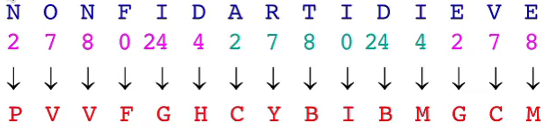
\includegraphics[scale=0.72]{img/9.PNG}
			\end{center}
			Ci conviene immaginare lo spazio di memoria come una sequenza di byte, ma organizzata in righe. Per via dell'\emph{endianess} conviene organizzare gli elementi nella direzione indicata nell'immagine. Supponiamo di avere il numero posto in fondo all'immagine: porremo le cifre meno significative nei posti con offset minore.
			
			\paragraph{Importanza dell'allineamento} Si capisce dall'ultimo esempio di accesso l'importanza dell'allineamento. Allineamento significa piazzare gli oggetti a confine di regioni grandi quanto l'oggetto. Fare questo ci garantisce che gli oggetti saranno contenuti in una stessa riga (un singolo accesso richiede centinaia di clock, quindi è importante non avere cose disallineate).
			
			\subsubsection{Organizzazione della RAM}
			\begin{center}
				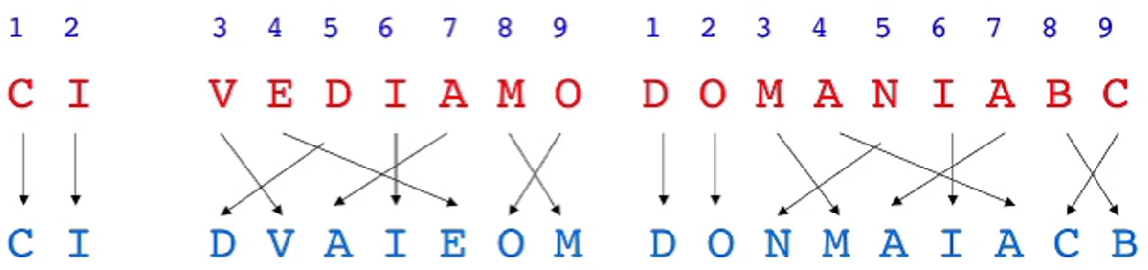
\includegraphics[scale=0.75]{img/10.PNG}
			\end{center} 
			La RAM deve essere organizzata per svolgere queste operazioni in parallelo.  
			\begin{itemize}
				\item Non possiamo collegare direttamente al bus un semplice modulo RAM con piedino di select, di lettura, e scrittura, fili di indirizzo e fili di dati. Ne dovremo collegare tanti quanti i byte che costituiscono l'intervallo. Ogni modulo rappresenta una colonna dello spazio di memoria.
				\item I moduli possono essere considerati alla pari delle RAM statiche viste a Reti logiche, ma dobbiamo tenere conto che le memorie moderne non sono fatte in quel modo. Approfondiremo la struttura circuitale delle memorie centrali moderne ad \emph{Elettronica digitale}.
				\item Abbiamo in ingresso:
				\small
				\begin{itemize}
					\item $n$ fili di indirizzo (SOLO per il numero di riga, non ho l'indirizzo completo);
					\item le variabili \emph{byte enabler}, che non vanno in ingresso a nessun circuito combinatorio (la logica combinatoria viene gestita dal processore);
					\item 64 fili di dati.
				\end{itemize}
				\normalsize
				\item I fili di dati sono ottenuti unendo insiemi di fili di dati: abbiamo $8$ fili provenienti da ciascun modulo (tanti quanti i bit che compongono il byte).
				\item Del numero di riga si fanno entrare:
				\small
				\begin{itemize}
					\item i $k$ bit meno significativi in ciascun modulo (dobbiamo dire in ciascun modulo quale elemento della colonna mi interessa, cioè quale riga);
					\item i bit rimanenti in una maschera che restituisce $0$ se la regione che vogliamo visitare si trova nel modulo RAM (non i sottomoduli, il modulo nel complesso).
				\end{itemize}
				\normalsize
				Ricordarsi, relativamente alla maschera, che lavoriamo con attivi bassi.
				\item Il valore per ciascun piedino di select è ottenuto da una porta OR che ha in ingresso l'uscita della maschera e il \emph{byte enabler} relativo\footnote{La dispensa di Lettieri pone la versione da me scritta qua (a mio parere la più intuitiva). Durante la spiegazione ha parlato di maschera con a valle una porta NOT, e di porte AND aventi in ingresso l'uscita negata della maschera e il relativo byte enabler.}.
			\end{itemize}
			\paragraph{In sostanza}
			\begin{itemize}
				\item Non si considerano i tre bit meno significativi, poichè abbiamo già i piedini \emph{byte enabler} a indicare quali posizioni ci interessano.
				\item Del numero di regione si prendono i $k$ bit meno significativi per determinare, in una colonna della RAM quale byte effettivamente ci interessa (l'offset dice cosa ci interessa orizzontalmente, i $k$ bit ciò che ci interessa verticalmente).
				\item I rimanenti bit, quelli più significativi, vanno in una maschera che determina se la RAM è interessata o no dall'operazione di lettura/scrittura (ricordare che tutte le componenti dell'architettura sono connesse sul bus, tutte ricevono e risponde solo chi è chiamato in causa).
			\end{itemize}
			\subsubsection{Osservazioni su lettura disallineata}  Prendiamo la seguente operazione
			\begin{verbatim}
				MOV 0x3ff, %RAX
			\end{verbatim}
			Il processore non fa solo due operazioni di lettura, ma deve anche riordinare gli elementi. Nella prima lettura avremo la parte meno significativa, nella seconda la più significativa. Dopo aver eseguito le due operazioni troveremo le parti invertite: la parte meno significativa nei byte più significativi del buffer, e così via. L'operazione è veloce e legata all'hardware (l'azione è eseguita dal processore e intrinseca nella MOV).
			\begin{center}
				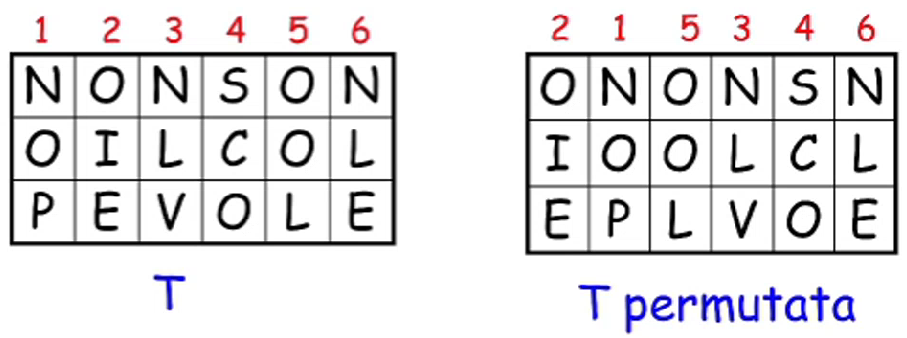
\includegraphics[scale=0.90]{img/11.PNG}
			\end{center} 
			\paragraph{Modifica di singoli bit} Per modificare un singolo bit dobbiamo
			\begin{itemize}
				\item Leggere l'intero byte
				\item Applicare una maschera con operazione logica (scegliamo la maschera in modo tale che si vada a modificare un solo bit)
				\item Scrivo il byte aggiornato
			\end{itemize}
			\begin{verbatim}
				MOV 0x3ff, %AL
				ORB $0x08, %AL <------- 00001000 OR %AL
				MOV $AL, 0x3ff
			\end{verbatim}
			In questo caso la modifica del singolo bit avviene via software. Per i dettagli ricordarsi gli esempi di operazioni viste a Reti logiche con le istruzioni macchina AND/OR/XOR.
			\paragraph{Formato di istruzioni e indirizzamento immediato} Il fatto che sorgente e destinatario non possano essere entrambi indirizzati in modo immediato è dovuto al formato di istruzioni: abbiamo spazio soltanto per un offset. L'unica alternativa è l'utilizzo di registri puntatori (nulla di nuovo rispetto a Reti logiche).
	\chapter{Martedì 09/03/2021}
\section{Iniziamo ad uccidere il compilatore}
\begin{itemize}
	\item Il file .o è un file di sistema che non dipende dal linguaggio compilato: posso partire da files .s, .cpp, .c...
	\begin{center}
		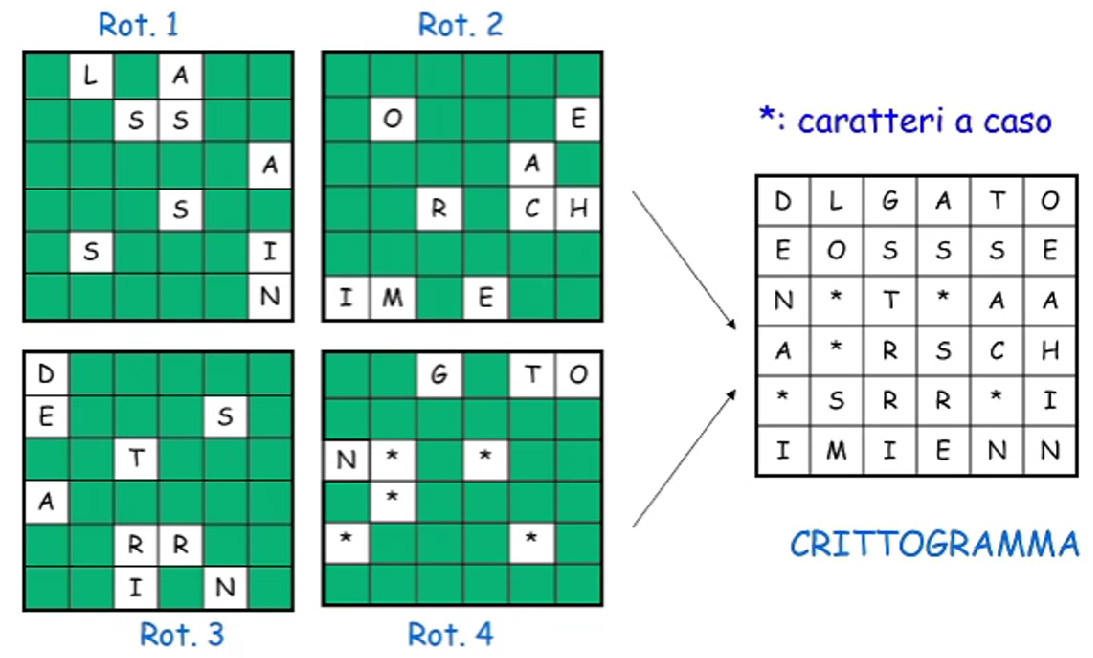
\includegraphics[scale=0.90]{img/12.PNG}
	\end{center} 
	\item Abbiamo due opzioni:
	\begin{itemize}
		\item scrivere un file in c o in c++, per esempio, passandolo da un compilatore che restituirà un file assembler;
		\item scrivere direttamente del codice assembler evitando il compilatore.
	\end{itemize}
	\item I comandi gcc e g++ non sono veri e propri compilatori, ma dei \emph{front-end}: capiscono quali strumenti devono utilizzare, e in che ordine, per ottenere l'eseguibile  finale.
\end{itemize}
\clearpage

\subsection{Esercizio dai lucidi del prof.Frosini} 
\paragraph{Testo}Vogliamo realizzare un programma diviso in due parti:
\begin{itemize}
	\item la prima col programma principale
	\item la seconda col sottoprogramma \emph{esamina}, usato dal primo file.
\end{itemize}
Il programma
\begin{itemize}
	\item legge caratteri fino al fine linea;
	\item per ogni carattere, oltre a stamparlo, chiama il sottoprogramma \emph{esamina}, e stampa il risultato prodotto da quest'ultimo.
\end{itemize}
Il sottoprogramma esamina restituisce otto caratteri in codifica ASCII, corrispondenti agli 8 bit della codifica del carattere ricevuto.

\small
\begin{multicols}{2}
	\paragraph{Codice di esamina.s}
	\begin{verbatim}
		.global esamina, alpha, beta
		
		.data
		alpha:  .byte 0
		.align 8  
		beta:   .quad 0
		
		.text
		esamina:
		push %rax
		push %rdx
		push %rcx
		
		mov alpha(%rip), %cl
		movabs beta, %rax
		mov $0, %rdx
		prossimo:
		test $0b10000000, %cl
		jz zero
		
		movb $'1', (%rax, %rdx)
		jmp avanti
		zero:
		movb $'0', (%rax, %rdx)
		jmp avanti
		avanti:
		shl %cl
		inc %rdx
		cmp $8, %rdx
		jb prossimo
		
		pop %rcx
		pop %rdx
		pop %rax
		ret
	\end{verbatim}
	\paragraph{Codice di codifica.s}
	\begin{verbatim}
		.include "ser.s"
		.global _start
		
		.data
		buffer:
		.fill 8,1
		
		.text
		_start:
		call tastiera
		cmp $'\n', %al
		je fine
		call video
		mov %al, alpha
		lea buffer, %rax
		mov %rax, beta(%rip)
		call esamina
		mov $' ', %al
		call video
		mov $0, %rcx
		ancora:
		mov buffer(,%rcx), %al
		call video 
		inc %rcx
		cmp $8, %rcx
		jb ancora
		
		mov $'\n', %al
		call video
		jmp _start
		fine:
		call uscita
	\end{verbatim}
\end{multicols}
\normalsize
\paragraph{Riflessioni}
\begin{itemize}
	\item \textbf{Trasmissione dei dati fra programma e sottoprogramma}. Dobbiamo utilizzare due variabili \emph{alfa} e \emph{beta} definite nel secondo file (\emph{extern} nel primo e \emph{global} nel secondo). La prima contiene il codice del carattere che il sottoprogramma deve esaminare, la seconda contiene l'indirizzo di una variabile array di 8 byte, dove il sottoprogramma deve porre il risultato. Il programma principale pone i dati in \emph{alfa} e \emph{beta}, quindi chiama \emph{esamina}.
	\item Abbiamo utilizzato una libreria contenuta nel file \emph{ser.s}. Per il momento il contenuto di questi sottoprogrammi non ci interessa (ne riparleremo più avanti).
	\item \textbf{Direttive \emph{global}}. Nel file \emph{esamina.s} le variabili \emph{alfa} e \emph{beta} sono dichiarate globali dalla seguente direttiva
	\begin{verbatim}
		.global esamina, alpha, beta
	\end{verbatim}
	se non facciamo questo l'altro file non potrà usare queste etichette. Ricordarsi che il collegatore vede solo ciò che è \emph{global}.
	\item \textbf{Reminiscenza di Reti logiche}. La PUSH e la POP devono essere utilizzate in modo adeguato (eseguo le push all'inizio del sottoprogramma, le pop alla fine del programma, inoltre per determinare l'ordine delle istruzioni POP considero l'ordine delle PUSH).
	\begin{verbatim}
		push %rax
		push %rdx
		push %rcx
		
		[...]
		
		pop %rcx
		pop %rdx
		pop %rax
		ret
	\end{verbatim}
	\begin{itemize}
		\item \textbf{Cosa succede se non eseguo le istruzioni pop alla fine?} L'istruzione RET alla fine del sottoprogramma \emph{esamina} prende l'indirizzo che sta in cima alla pila: il problema è che abbiamo eseguito la push altre tre volte dopo la chiamata del sottoprogramma, quindi l'elemento in cima alla pila non è quello che dovrebbe usare la RET. Se l'indirizzo considerato (quello che si cerca di trattare come indirizzo) ci porta a un'area non assegnata al programma otterremo l'errore di \emph{segmentation fault}.
		\item \textbf{Cosa succede se poniamo le POP in ordine non consueto?} I registri non vengono riportati al loro valore originario. L'errore non viene segnalato, ma può provocare risultati indesiderati.
	\end{itemize}
	\item \textbf{Sintassi per gli indirizzi}. Attenzione alla rip
	\begin{verbatim}
		mov alpha(%rip), %cl
	\end{verbatim}
	Siamo certi che questo indirizzamento ci permette di evitare problemi. La cosa non è necessaria in questo caso: il programma è molto piccolo.
	\item \textbf{Istruzione \emph{test} in \emph{esamina.s}}. L'istruzione
	\begin{verbatim}test $0b10000000, %cl\end{verbatim}
		equivale all'istruzione AND, ma non viene modificato il destinatario. L'unica cosa modificata sono i flag. 
		\item \textbf{Sostituzione automatica della \emph{mov} con la \emph{movabs}}. Se poniamo qualcosa che non è rappresentabile su 32 bit
		\begin{verbatim}
			mov $0x12345668, %rax
		\end{verbatim}
		l'assemblatore adotta automaticamente la movabs (il destinatario è un registro, nient'altro). Provare per credere!
		\begin{framed}
			\item \textbf{Azzeramento della parte alta di un registro a 64 bit}. Se il registro è a 32 bit la parte alta viene sempre azzerata (\underline{novità}). Segue che le seguenti istruzioni\begin{verbatim}
				mov $0, %edx
				mov $0, %rdx
			\end{verbatim}
			avranno lo stesso effetto
		\end{framed}
		\item \textbf{Natura dell'operando destinatario} (banalità importante). Possiamo scrivere...? \begin{verbatim}cmp %rdx, $8\end{verbatim} 
			No: la destinazione è per natura un registro o un indirizzo in memoria (sempre, anche se l'istruzione non ci scrive) 
			\item \textbf{Domanda da pretest di Reti logiche}. Cosa fa la seguente istruzione..?
			\begin{verbatim}
				mov $beta, %rax
			\end{verbatim}
			La stessa cosa della LEA: pone come contenuto del registro rax l'indirizzo relativo all'etichetta \emph{beta}. Possiamo fare la stessa cosa così:
			\begin{verbatim}lea beta, %rax\end{verbatim}
				\item \textbf{Allineamento e disallineamento}. Attenzione ai dati
				\begin{verbatim}
					.data
					alpha:  .byte 0
					beta:   .quad 0
				\end{verbatim}
				Sono disallineati: \emph{alpha} si trova all'offset 0, \emph{beta} all'offset 1. Segue che un byte di \emph{beta} si troverà in un'altra regione naturale (dunque sono necessari due accessi). L'assemblatore non interviene, a meno che non poniamo la seguente direttiva
				\begin{verbatim}
					.data
					alpha:  .byte 0
					.align 8
					beta:   .quad 0
				\end{verbatim}
				La direttiva mi permette \emph{di scartare i prossimi elementi in modo tale da arrivare al prossimo multiplo di 8}.
				\begin{center}
					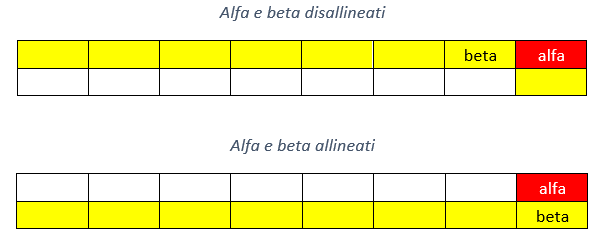
\includegraphics[scale=.85]{img/149.PNG}
				\end{center} 
				\item \textbf{Etichette esterne}. L'assemblatore per default assume che tutte le etichette non definite in un file siano \emph{esterne}, cioè definite in un file esterno. Possiamo indicarlo in modo esplicito con una direttiva
				\begin{verbatim}
					.extern alpha
				\end{verbatim}
				Il linker, che ha visione completa (in contrasto all'assemblatore), inchioda se si accorge che certe etichette non sono state definite.
				\begin{itemize}
					\item \textbf{Cosa succede se non uso global per segnalare ad altri files ulteriori etichette?} Si segnala errore di \emph{undefined reference} dopo aver avviato il linker. L'etichetta è definita (si veda \emph{nm}), ma non viene vista nell'altro file.
					\item \textbf{Cosa succede se dichiaro un'etichetta beta globale in esamina.s e ne introduco una con lo stesso nome in codifica.s?} Se un file presenta un'etichetta con un certo nome e questa viene usata nel file stesso non c'è motivo per andarla a cercare altrove. \underline{Quella che avviene è una \emph{sovrapposizione} rispetto alla variabile} \underline{globale dichiarata altrove}.
				\end{itemize}
			\end{itemize}
			
			\chapter{Giovedì 11/03/2021}
			\section{Programmi misti C++/Assembler}
			Oggi vogliamo cominciare a scrivere programmi misti, cioè scritti in parte in C++ (passati dal compilatore) e in parte in Assembler. 
			
			\subsection{g++ e \emph{startfiles}} Il g++ è un front-end per i vari strumenti preconfigurato per programmi scritti in C++. Capisce cosa deve fare e chiama opportunamente compilatore e/o assemblatore (in base ai files che gli passiamo)
			\begin{verbatim}
				g++ -o nome_file_output -no-pie file1, file2, ...
			\end{verbatim}
			creiamo un eseguibile con nome \emph{codifica} a partire dai files indicati nel comando. Il parametro \emph{-no-pie} viene posto per evitare degli errori (non approfondiremo il perché).  
			\paragraph{Proviamolo} Proviamo ad eseguire g++ con il programma scritto durante la scorsa lezione 
			\begin{verbatim}
				g++ -o codifica -no-pie codifica.s esamina.s
			\end{verbatim}
			creiamo un eseguibile con nome \emph{codifica} a partire dai file \emph{codifica.s}, \emph{esamina.s}. Il terminale ci segnala errore:
			\begin{center}
				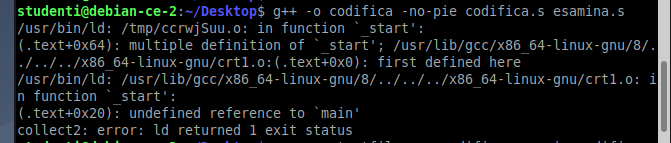
\includegraphics[scale=.9]{img/150.PNG}
			\end{center} 
			\paragraph{Come mai?} g++ aggiunge, senza dire nulla, degli \emph{start files} che fanno delle inizializzazioni (fatte prima della partenza del programma vero e proprio): in questi file oggetto aggiuntivi viene definito \emph{$\_$start}, che fa un po' di cose e chiama, alla fine, la funzione \emph{$\_$main}. Possiamo evitare questi inserimenti ponendo un ulteriore parametro nell'istruzione
			\begin{verbatim}
				g++ .nostartfiles -o codifica -no-pie codifica.s esamina.s
			\end{verbatim}
			Se facciamo questa cosa col problema visto nella scorsa lezione tutto funziona regolarmente. Non avendo utilizzato cose non nostre non ci sono problemi nell'ignorare gli \emph{startfiles}.
			\paragraph{Cosa potrebbe fare la start?}
			\begin{itemize}
				\item Definire strutture e classi (se io dichiaro un'istanza globale di una classe dovrò avere già definita la classe al momento dell'esecuzione di main)
				\item Inizializzazione di oggetti cin e cout (che, va be, sono classi)
				\item Esecuzione dei distruttori
			\end{itemize}
			\paragraph{Standard C++}  Definiamo \emph{main} invece di \emph{start} e poniamo RET alla fine del programma. Abbiamo una chiamata del sottoprogramma main all'interno di start: dopo che main ha restituito il controllo la start esegue quanto necessario per concludere l'esecuzione del programma, incluso i distruttori.
			\subsection{g++ e \emph{overloading}}
			\paragraph{Scriviamo l'analogo in C++ di codifica.s}
			\begin{verbatim}
				#include <iostream>
				
				extern char alpha; 
				extern char* beta;
				extern void esamina();
				
				char buffer[8];
				
				int main() {
					while(true) {
						char c;
						std::cin.get(c);
						
						if(c == `\n')
						break;
						
						alpha = c; <--- devo dire al compilatore chi e' alpha          [LO FACCIO SOPRA]
						beta = buffer; <--- devo dire al compilatore chi e' beta
						
						esamina(); <-- devo dire al compilatore chi e' esamina
						for(int i = 0; i < 8; i++) {
							std::cout << buffer[i];
						}
						std::cout << "\n";
					}
				}
			\end{verbatim}
			\clearpage
			\noindent Se eseguiamo il codice
			\begin{verbatim}
				g++ -no-pie -o codifica1 codifica1.cpp esamina.s
			\end{verbatim}
			si lamenta perché non trova \emph{esamina}. 
			\begin{center}
				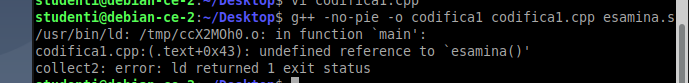
\includegraphics{img/151.PNG}
			\end{center} 
			Vediamo cosa succede controllando gli elementi definiti in codifica1.cpp
			\begin{verbatim}
				g++ -c codifica1.cpp <---- mi limito ai files oggetto
				nm codifica1.o <---- leggo simboli definiti
			\end{verbatim}
			\begin{center}
				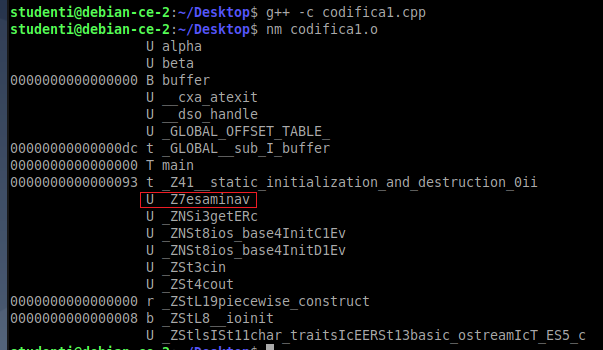
\includegraphics{img/152.PNG}
			\end{center} 
			troviamo esamina, ma con un nome strano.
			\paragraph{Causa} Il compilatore storicamente ha sempre usato gli stessi collegatori del C. Sappiamo che differenza sostanziale tra C e C++ è la presenza dell'overloading nel secondo (cioè funzioni con nome uguale e parametri diversi). Nel nostro caso l'etichetta per esamina è la seguente
			\begin{verbatim}
				_Z7esaminav
			\end{verbatim}
			$\_$Z è un prefisso obbligatorio, 7 è il numero di caratteri del nome della funzione, v significa void (cioè assenza di parametri). Non possiamo gestire più funzioni con lo stesso nome mediante le stesse etichette, dobbiamo differenziarle! 
			\paragraph{Soluzione}
			\begin{itemize}
				\item O modifico l'extern ponendo quel nome strano (vedremo più avanti le convenzione relative ai nomi delle etichette in C++)
				\begin{verbatim}
					extern void _Z7esaminav();
				\end{verbatim}
				\item O pongo l'extern nel seguente modo
				\begin{verbatim}
					extern "C" void esamina();
				\end{verbatim}
				esiste \emph{una funzione esamina che non ha argomenti, posta in un altro file, e scritta in C} (ok, non è scritta in C, ma rispetta lo standard del C). Nel C non esiste l'overloading, quindi le etichette assumono il nome che ci aspettiamo.
			\end{itemize}
			Chiaramente non serve questa cosa per le altre extern: non esiste l'overloading per le variabili.
			\paragraph{Analogo in C++ di esamina.s}
			\begin{verbatim}
				char alpha;
				char* beta;
				
				extern "C" void esamina() { <-- extern serve solo per poter indicare "C", 
					<-- altrimenti abbiamo il problema di prima
					char c = alpha;
					for(int i = 0; i < 8; i++) {
						if(c & 0x80) {
							beta[i] = `1';
						}
						else {
							beta[i] = `0';
						}
						c << 1;
					}
				}
			\end{verbatim}
			
			\paragraph{E se volessimo solo l'assembler?} Poniamo l'istruzione così
			\begin{verbatim}
				g++ -fno-PIC -S codifica1.cpp <-- genero l'assembler
				vi codifica1.s <---- apro l'assembler
			\end{verbatim}
			Il codice ottenuto presenta le istruzioni Assembler che ci aspettiamo, più delle righe di codice contenenti principalmente informazioni (utili, per esempio, al debugger).
			
			\clearpage \subsection{Uso dei registri} 
			Vogliamo trovare un compromesso tra funzione chiamante e funzione chiamata: in particolare, vogliamo garantire al chiamante un certo numero di registri.
			
			\begin{center}
				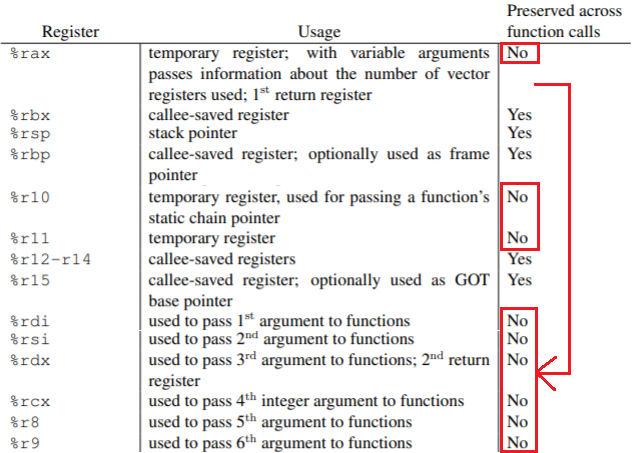
\includegraphics{img/269.PNG}
			\end{center} 
			\begin{itemize}
				\begin{framed}
					\item Alcuni registri sono detti \emph{scratch}, cioè possono essere usati liberamente dalla funzione chiamata senza dover salvare il contenuto pre-esistente:
					\begin{itemize}
						\item RAX, R10, R11, \underline{RCX, RDX, RSI, RDI, R8, R9} {\small (Per ricordare: A,C,D,S,8,9,10,11)}.
					\end{itemize}
					\item I registri rimanenti sono registri \emph{non scratch}, garantiti al chiamante (quindi non vengono toccati dalla funzione chiamata): RBP, RBX, R12, R13, R14, R15. 
				\end{framed}
				\item \textbf{Conseguenza}: dobbiamo stare attenti, il contenuto dei registri scratch non viene mantenuto in caso di chiamate di funzione. Noi dobbiamo preoccuparci esclusivamente dei nostri contenuti, dunque ricorrere alle istruzioni PUSH e POP se non vogliamo perdere il valore di alcuni registri scratch a seguito di chiamata di funzione.
			\end{itemize}
			\clearpage 
			
			\subsection{Rappresentazione dei dati}
			La cosa è molto intuitiva, ma c'è uno standard da eseguire. 
			\subsubsection{Tipi fondamentali} 
			Sono disponibili molte informazioni su \url{cppreference.com} alla voce \emph{Fundamental types}.
			\begin{center}
				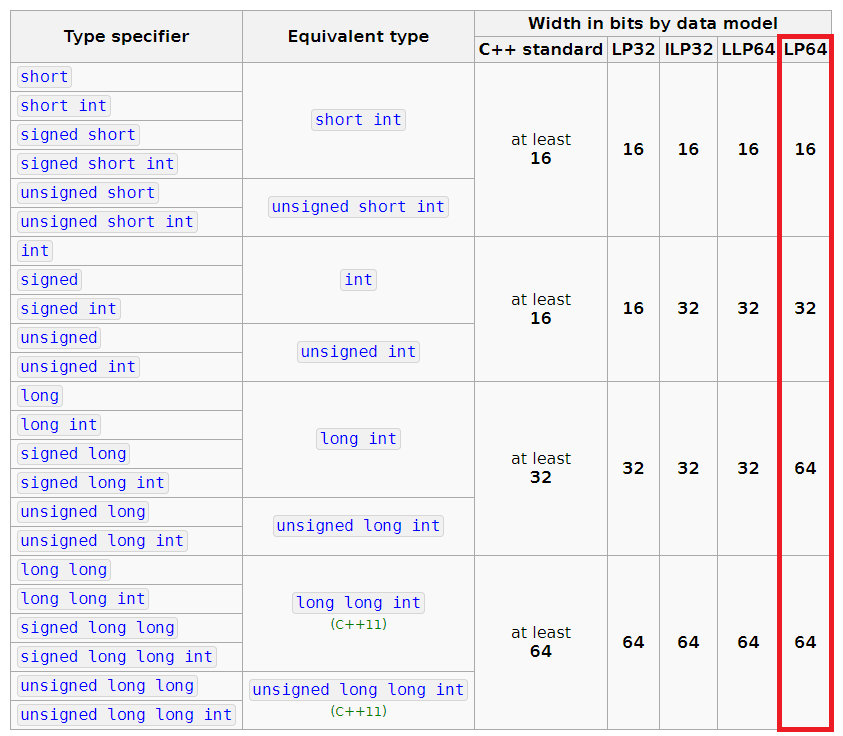
\includegraphics[scale=0.90]{img/13.PNG}
			\end{center} 
			Il sito mette insieme standard e implementazione: in particolare si osserva che lo standard da margini di liberta all'implementatore (si parla di \emph{almeno}, non un numero ben preciso). Questo significa che altri documenti dovranno specificare per intero come avviene l'implementazione. Sono riportate alcune implementazioni comuni nello standard. In particolare ci interessano LLP64 ed LP64: la prima è per windows, la seconda per i sistemi Unix e Unix-like (Linux, macOs).
			\clearpage 
			
			\paragraph{char} Cosa strana è la presenza di tre tipi diversi:
			\begin{itemize}
				\item \begin{verbatim}
					signed char
				\end{verbatim}
				tipica rappresentazione dei char in x86, x64.
				\item \begin{verbatim}
					unsigned char
				\end{verbatim}
				\item \begin{verbatim}
					char
				\end{verbatim}
				la rappresentazione sarà equivalente a signed char o unsigned char, ma rimane un tipo diverso.
			\end{itemize}
			\paragraph{Approfondiamo l'implementazione} Il documento che specifica tutto ciò che lo standard non dice (in Linux) è il \emph{System V Application Binary Interface}. Per quanto riguarda la rappresentazione dei dati abbiamo una tabella con tipi, dimensioni e allineamento. Caratteristica dei tipi fondamentali è avere dimensione e allineamento uguali.
			\begin{center}
				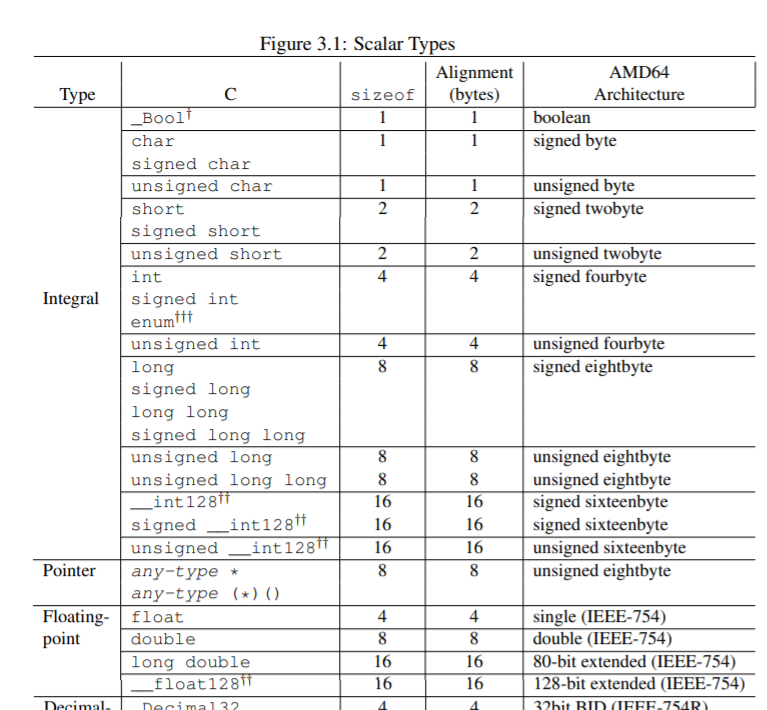
\includegraphics[scale=0.85]{img/14.PNG}
			\end{center} 
			\clearpage 
			
			\subsubsection{Tipi derivati}
			Quale dimensione e allineamento avranno i tipi derivati?
			\begin{itemize}
				\item \textbf{Puntatori}: hanno dimensione fissa al di la di cosa puntano, quindi valgono le cose già viste nella pagina precedente.
				\item  \textbf{Array}: \begin{verbatim}
					tipo a[DIM]
				\end{verbatim}
				\begin{multicols}{2}
					\begin{itemize}
						\item \emph{sizeof}: $\text{DIM} * \text{sizeof}(\text{tipo})$
						\item \emph{alignof}: $\text{alignof}(\text{tipo})$
					\end{itemize}
				\end{multicols}
				%\begin{center}
				%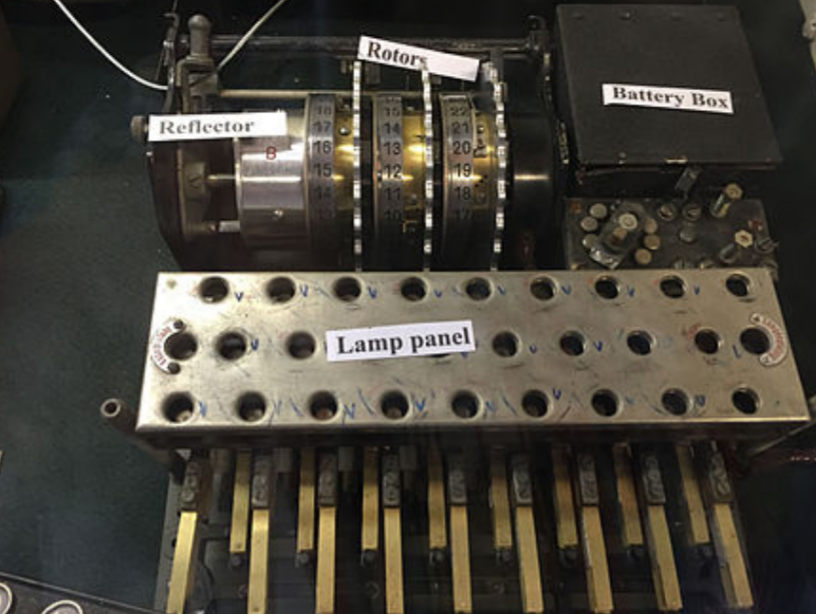
\includegraphics[scale=0.75]{img/15.PNG}
				%\end{center} 
				gli indirizzi crescenti, che partono da zero, mi rendono facile il calcolo dell'indirizzo di ogni elemento dell'array.
				
				\item \textbf{Strutture}: la cosa è un tantino più complicata.
				
				\begin{verbatim}
					struct s {
						tipo_1 f_1;
						tipo_2 f_2;
						tipo_3 f_3;
					}
				\end{verbatim}
			\begin{itemize}
					\item \emph{alignof}: \[\max_i\, \{ \text{alignof}(\text{tipo$_i$})\}\]
					\item \emph{sizeof}: non esiste una formula vera e propria, per prima cosa dobbiamo immaginarci il \emph{layout} della struttura. Consideriamo che:
					\begin{itemize}
						\item ogni elemento della struttura deve rispettare il proprio allineamento; 
						\item i campi devono trovarsi in memoria \textbf{nell'ordine in cui sono dichiarati} (non esistono forme di ottimizzazione in cui viene alterato l'ordine degli elementi);
						\item la dimensione totale della struttura deve essere un multiplo dell'allineamento della struttura.
					\end{itemize}
				\end{itemize}
			\end{itemize}
			\subsubsection{Primo esempio di struttura}
			\begin{center}
				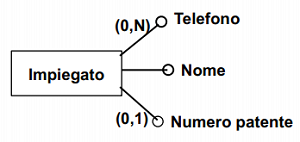
\includegraphics[scale=0.80]{img/16.PNG}
			\end{center} 
			\begin{itemize}
				\item Gli interi hanno dimensione $4$ e allineamento $4$. L'ordine in cui sono stati posti mi permette di porre i due interi nella stessa regione naturale. Il long ha dimensione $8$ e allineamento $8$. Dobbiamo allocarlo al primo indirizzo, multiplo di 8, successivo. 
				\item \textbf{Conclusioni}:\begin{itemize}
					\item \emph{alignof}: il massimo degli allineamenti è $8$.
					\item \emph{sizeof}: $16$ byte
				\end{itemize}
			\end{itemize}
			%\begin{itemize}
			%\item Contrariamente all'assemblatore il compilatore vuole conoscere tutte le etichette esistenti. Dobbiamo indicarlo noi con \emph{extern}.
			%\end{itemize}
			\subsubsection{Secondo esempio di struttura}
			\begin{center}
				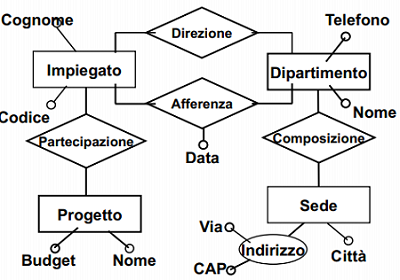
\includegraphics[scale=0.80]{img/17.PNG}
			\end{center} 
			\begin{itemize}
				\item Contrariamente a prima non possiamo mettere il char assieme a un altro elemento: nè con long (che ha dimensione di 8 byte), nè con char (che si trova dopo long). L'allineamento è stringente e impone che il long sia posto in un indirizzo multiplo di 8. Seguono 7 byte inutilizzati nella regione dove si trova il primo char.
				\item Dopo long mettiamo l'altro char, che non pone particolari vincoli. Rimangono 7 byte (che non faranno parte della struttura).
				\item \textbf{Conclusioni}:\begin{itemize}
					\item \emph{alignof}: $8$ (il massimo tra gli alignof, il più alto è quello di long)
					\item \emph{sizeof}: $17$ byte, più $7$ byte non utilizzati.
				\end{itemize}
			\end{itemize}
			
			\paragraph{perché non si può ottimizzare l'ordine degli elementi?} Il compilatore non può ottimizzare l'ordine degli elementi per conto suo. 
			\begin{itemize}
				\item Supponiamo di avere due files distinti. Il compilatore lavora distintamente su questi due. 
				\item Se la struttura dipendesse dalle ottimizzazioni i due files potrebbero aver adottato ottimizzazioni diverse, quindi le due strutture non risulterebbero equivalenti.
				\item Se nei due files ci sono funzioni che comunicano tra di loro e che devono scambiarsi una struttura allora i due files devono concordare sul \emph{layout} della struttura.
			\end{itemize}
			
			\subsubsection{Terzo esempio di struttura}
			Prendiamo il seguente esempio
			\begin{center}
				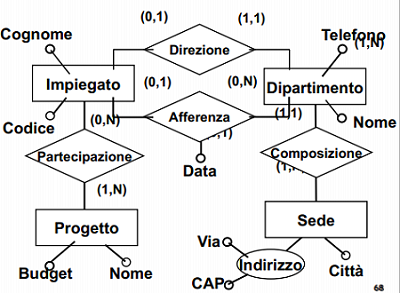
\includegraphics[scale=0.80]{img/18.PNG}
			\end{center} 
			L'unica cosa che conta è l'ordine degli elementi. Si consideri che l'allineamento di ogni singolo char di $s$ è $1$, quindi l'allineamento della struttura $s$ è $1$. Possiamo porre i byte di $s$ subito, senza passare subito a una nuova regione (niente ce lo vieta).
	\chapter{Venerdì 12/03/2021, Lunedì 15/03/2021 e Martedì 16/03/2021}

\section{Programmazione mista: funzioni}
Per scrivere funzioni in C++ e chiamarle da Assembler, e viceversa, dobbiamo tener conto di una serie di regole, in particolare dobbiamosapere come avviene il passaggio dei parametri (in ingresso e in uscita) e dove vengono poste le variabili locali. La soluzione adottata è sofisticata (non è la prima cosa che viene in mente a una funzione).

\paragraph{Cosa serve a una funzione?}
Una qualunque funzione avrà bisogno di:
\begin{itemize}
	\item uno spazio per i parametri in ingresso, in uscita, e i risultati intermedi;
	\item uno spazio per le istruzioni.
\end{itemize}
%La cosa può essere immaginata in modo molto elementare
%\begin{center}
%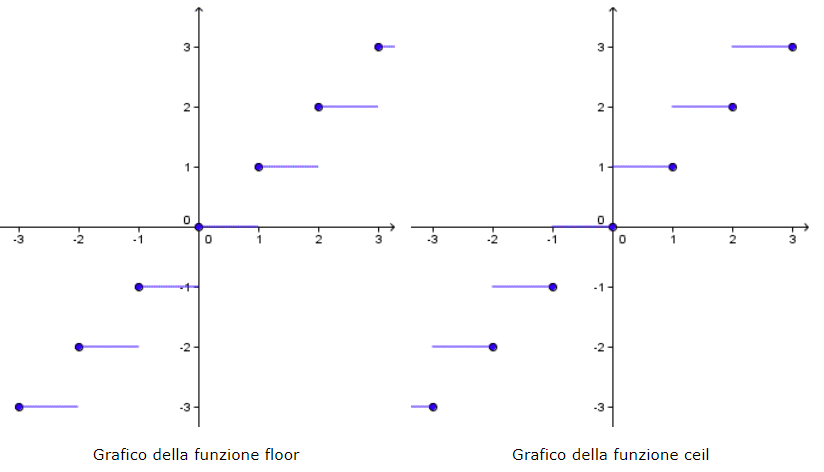
\includegraphics[scale=0.90]{img/19.PNG}
%\end{center} 
\paragraph{Preallocazione?} La preallocazione dello spazio per parametri e risultati intermedi è svantaggiosa: 
\begin{itemize}
	\item si consuma troppo spazio;
	\item non è possibile fare chiamate ricorsive della stessa funzione;
	\item non è possibile condividere lo stesso codice in simultanea a più flussi.
\end{itemize}

\paragraph{Quindi?} L'idea è di mettere questi parametri su una pila, ponendo il cosiddetto \emph{record di attivazione}.
\clearpage 
\subsection{Record di attivazione}
Ogni volta che si chiama una funzione si alloca nella pila il cosiddetto \emph{record di attivazione della funzione}, che contiene variabili locali, parametri, e l'indirizzo di ritorno.
\begin{center}
	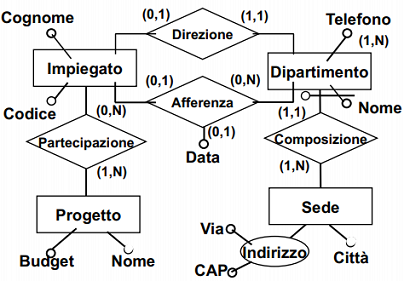
\includegraphics[scale=0.59]{img/20.PNG}
\end{center} 
L'indirizzo di ritorno è cosa già vista: lo inserisco in pila con la CALL e lo rimuovo con la RET. La funzione accede ai vari campi del record di attivazione in modo indiretto. Dobbiamo tener conto che l'indirizzo di questi elementi non è fisso, considerando che potrei avere altre chiamate ricorsive prima di quella attuale che stiamo considerando. Una soluzione è calcolare l'offset rispetto al registro rsp
\begin{verbatim}
	offset(%rsp)
\end{verbatim}
rimane il fatto che se durante l'esecuzione del programma alteriamo la RSP allora gli offset dovranno essere ricalcolati. I processori moderni lo sanno fare senza grossi problemi.
\paragraph{Architettura Intel} Nell'architettura Intel si tende a usare un registro esplicito che punti al record di attivazione senza usare rsp. Introduciamo il registro RBP (\emph{Register Base Pointer}): per tutta la durata di esecuzione della funzione il valore di questo registro è costante e punta a un punto preciso del record di attivazione, subito sopra l'indirizzo di ritorno. Ad ogni chiamata di funzione viene memorizzato il valore precedente di rbp mediante PUSH.
\begin{verbatim}
	PUSH %rbp <--- salvo il valore vecchio 
	MOV %rsp, %rbp <--- aggiorno il contenuto del registro
\end{verbatim}
alla fine dell'esecuzione, se RSP è stato riportato al suo valore iniziale, diremo
\begin{verbatim}
	POP %rbp <--- recupero il valore vecchio 
	RET
\end{verbatim}
Nel caso in cui ciò non avvenga basta eseguire un'istruzione MOV (non ne avremo bisogno, basta rispettare le regole sull'uso di PUSH e POP). Per terminare il record di attivazione basta riservare spazio per i parametri e le variabili locali. Questo è semplice
\begin{verbatim}
	SUB $spazio, %rsp
\end{verbatim}
Sposto rsp in modo che successive push o chiamate di funzione proseguano oltre senza toccare questo spazio. La struttura del record di attivazione (relativamente a parametri e variabili locali) è flessibile: il suo contenuto interessa solo alla funzione.

\subsubsection{Passaggio di parametri in ingresso}  Altra cosa che deve fare il chiamante è passare i parametri. Chiaramente non può scriverli nel record di attivazione direttamente, visto che si muoverà prima che venga riservata l'area di memoria. Osserviamo le differenze tra le due architetture
\begin{itemize}
	\item \textbf{Architettura a 32bit}: i parametri vengono posti nella pila prima di eseguire la call
	\begin{framed}
		\item \textbf{Architettura a 64bit}: sfruttando il numero più alto di registri si passa i parametri direttamente con questi. Possiamo avere varie situazioni
		\begin{itemize}
			\item Pongo i parametri nei registri e li mantengo qua senza spostarli nell'aria di memoria
			\item Pongo i parametri nei registri e li sposto nell'area di memoria dedicata ai parametri e alle variabili locali. In quali occasioni sono costretto a fare così?
			\begin{itemize}
				\item Quando devo chiamare altre funzioni, oppure
				\item quando devo utilizzare istruzioni che ricorrono per forza a certi registri (moltiplicazione, divisione, istruzioni per le stringhe)
			\end{itemize}
		\end{itemize}
		se la funzione ha più di 6 argomenti si adotta, per gli argomenti in eccesso, la strategia vista per l'architettura a 32bit. Si usano i seguenti registri, nell'ordine seguente...
		\begin{multicols}{3}
			\begin{enumerate}
				\item \%RDI
				\item \%RSI
				\item \%RDX
				\item \%RCX
				\item \%R8
				\item \%R9
			\end{enumerate}
		\end{multicols}
		(D,S,D,C,8,9) Abbiamo già indicato questi registri come registri scratch: quali registri scratch possiamo usare dipenderà dalle situazioni.
	\end{framed}
\end{itemize}

\paragraph{Osservazione} Argomenti diversi usano registri diversi. Se io ho, per esempio... 
\begin{verbatim}
	f(char c, char b);
\end{verbatim}
non posso metterli nello stesso registro: c va in rdi, b in rsi.\\

\noindent \textbf{Esempio di situazione in cui i parametri non vengono mantenuti nei registri}

\begin{multicols}{3}
	\begin{verbatim}
		struct s {
			int i[4];
		}
	\end{verbatim}
	\begin{verbatim}
		int f(s x) {
			g(&x);
		}
	\end{verbatim}
	\begin{verbatim}
		g(s* p) {
			...
		}
	\end{verbatim}
\end{multicols}
\noindent Non possiamo tenere il parametro solo nei registri, visto che questi non hanno indirizzo. Devo spostare il contenuto della struttura in memoria, a quel punto, avrò qualcosa che potrò puntare a partire dalla mia funzione.

\subsubsection{Parametro in uscita} La funzione termina: dove pongo il risultato? Abbiamo due possibilità
\begin{verbatim}
	%RAX
	%RDX_%RAX <--- (In caso di estensione)
\end{verbatim} 
O utilizzo solo il registro rax, oppure utilizzo anche il registro rdx (ponendo in rdx la parte più significativa di ciò che voglio restituire.\\
\scriptsize

\noindent \textbf{Hey} Questa cosa dovrebbe accenderci la lampadina.
\begin{verbatim}
	XOR %EAX, %EAX ----------> return 0;
\end{verbatim}
Stea ci ha detto che per convenzione si pone questa istruzione al termine del programma. Adesso capiamo perché!
\normalsize
\paragraph{Osservazione sulla dimensione dei parametri in ingresso e in uscita} 
\begin{itemize}
	\item Se io passo in ingresso una struttura e questa è grande al più 16 byte, questa dovrà essere passata con uno o due registri (la prima riga va in rdi, la seconda in rsi). 
	\item Se la struttura in ingresso è più grande di 16 byte la cosa è più complicata, ne riparleremo più avanti. 
\end{itemize}
Stesso ragionamento vale nella restituzione (con i registri citati prima).




\subsection{Esempio di struttura passata come parametro in ingresso}
\begin{center}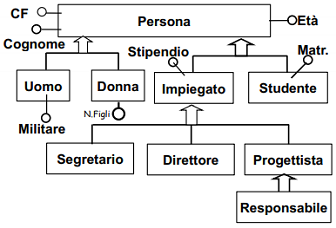
\includegraphics[scale=0.85]{img/22.PNG}\end{center}
\begin{verbatim}
	struct s {
		int i[4];
	}
	int f(s x) {
		int sum = 0;
		for(int j = 0; j < 4; j++)
		sum += x.i[j];
		return sum;
	}
\end{verbatim}
Il contenuto dell'elemento s sarà diviso tra rdi ed rsi. La cosa ottenuta non è molto comoda:
\begin{itemize}
	\item i[0] e i[2] possono essere recuperati, rispettivamente, coi registri EDI ed ESI
	\item ma gli altri due elementi?
\end{itemize}
L'unica cosa possibile è shiftare.


\subsection{Esercizio dalle diapositive del prof.Frosini}
\begingroup
\small
\subsubsection{Passaggio di parametri per valore (pag.35)}
\begin{framed}
	\noindent \textbf{Codice c++}
	\begin{multicols}{2}
		\begin{verbatim}
			// programma sommmaintGlob, file es1a.cpp
			#include"servi.cpp"
			extern "C" int elab1(int n, int m);
			int alfa, beta;
			int main() { 
				int ris;
				alfa = leggiint(); 
				beta = leggiint();
				ris = elab1(alfa, beta);
				scriviint(ris); 
				nuovalinea();
				return 0;
			};
			
			// programma sommmaintGlob, file es1b.cpp
			extern "C" int elab1(int n1, int n2) { 
				int i, j;
				i = n1+n2;
				j = n1-n2;
				
				return i*j;
			};
		\end{verbatim}
\end{multicols}\end{framed}
\noindent \textbf{Funzione \emph{elab1} in Assembler}
\begin{multicols}{2}
	\begin{verbatim}
		.global elab1
		elab1:
		push %rbp
		mov %rsp, %rbp
		sub $16, %rsp
		
		mov %edi, -8(%rbp)
		mov %esi, -4(%rbp)
		
		# i = n1 + n2
		mov %edi, -16(%rbp)
		add %esi, -16(%rbp)
		
		# j = n1 - n2
		mov %edi, %eax
		sub %esi, %eax
		mov %eax, -12(%rbp)
		
		# return i*j
		imull -16(%rbp), %eax
		
		leave   
		ret
	\end{verbatim}
\end{multicols}

\begin{itemize}
	\item Per prima cosa gestiamo il registro RBP 
	\begin{verbatim}
		push %rbp
		mov %rsp, %rbp
	\end{verbatim}
	salviamo in pila il valore vecchio e aggiorniamo il registro con l'RSP attuale.
	\item Riserviamo lo spazio per le variabili locali e i parametri di ingresso
	\begin{verbatim}
		sub $16, %rsp
	\end{verbatim}
	Riempiamo lo spazio appena allocato:
	\begin{center}
		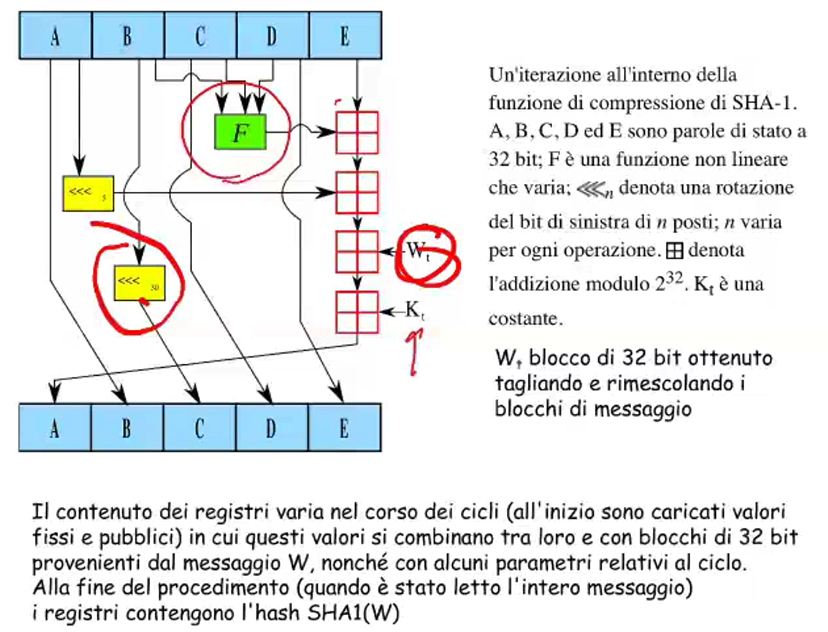
\includegraphics[scale=.85]{img/33.PNG}
	\end{center} 
	nell'indirizzamento si deve fare riferimento ad RBP (in questo caso potrei fare riferimento anche ad RSP, ma in generale è rischioso farlo). I registri source sono quelli che abbiamo citato, utilizzati nell'ordine indicato (in questo caso RDI ed RSI). 
	\begin{verbatim}
		mov %edi, -8(%rbp)
		mov %esi, -4(%rbp)
	\end{verbatim}
	Abbiamo due \emph{int} in ingresso, dunque bastano le parti meno significative a 32 bit.
	\begin{framed}
		\item \textbf{Domanda}. Come capisco quale sia il destinatario di queste istruzioni? Mi basta sommare il numero a destra con quello in alto. Riguardo la seconda MOV la tentazione potrebbe essere scrivere quanto segue
		\begin{verbatim}
			mov %esi, -12(%rbp)
		\end{verbatim}
		Ricordarsi che siamo in una pila, dunque andiamo indietro e non in avanti. 
		\begin{center}
			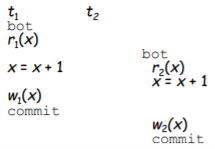
\includegraphics[scale=.65]{img/153.PNG}
		\end{center} 
	\end{framed}
	\item Rappresentiamo l'addizione tra $n1$ ed $n2$ così
	\begin{verbatim}    
		mov %edi, -16(%rbp)
		add %esi, -16(%rbp)
	\end{verbatim}
	Nell'indirizzo di \emph{i}, cioè nell'indirizzo della variabile dove finisce la somma, procedo in due step:
	\begin{enumerate}
		\item pongo come contenuto \emph{n1}, che sta in ESI;
		\item sommo al contenuto la variabile \emph{n2}, che sta in EDI.
	\end{enumerate}
	\item Rappresentiamo la sottrazione tra $n1$ ed $n2$: so che il primo è il minuendo, e il secondo il sottraendo. Pongo il minuendo in EAX
	\begin{verbatim}
		mov %edi, %eax
		sub %esi, %eax
		mov %eax, -12(%rbp)
	\end{verbatim}
	Il passaggio da EAX è necessario per fare la moltiplicazione poco dopo.
	\item Attenzione all'istruzione utilizzata: $i$ e $j$ sono due interi, non possiamo utilizzare la istruzione MUL per i numeri naturali (ignorerebbe il segno).  
	\begin{verbatim}
		imull -16(%rbp), %eax
	\end{verbatim}
	Novità!!!! La IMUL ha due operandi: si moltiplica il sorgente per il destinatario e si pone il risultato nel destinatario.
	\item Prima di concludere dobbiamo disfare quanto fatto nel prologo. Lo facciamo con la seguente istruzione
	\begin{verbatim}
		leave
	\end{verbatim}
	adesso concludiamo con la solita istruzione
	\begin{verbatim}
		ret
	\end{verbatim}
\end{itemize}
\paragraph{Traduciamo anche il main}
\begin{verbatim}
	# int alfa, beta;
	.data
	alfa:
	.long 0
	beta:
	.long 0
	
	.text
	.global main
	main:
	push %rbp
	mov %rsp, %rbp
	sub $16, %rsp # int ris, tenendo conto delle cose dette (vedere sotto)
	
	# alfa = leggiint();
	call leggiint # risultato in %rax
	mov %eax, alfa(%rip)
	
	# beta = leggiint();
	call leggiint # risultato in %rax
	mov %eax, beta(%rip)
	
	# ris = elab1(alfa, beta);
	mov alfa(%rip), %edi
	mov beta(%rip), %esi
	call elab1
	mov %eax, -8(%rbp)
	
	# scriviint(ris);
	mov -8(%rbp), %edi
	CALL scriviint
	
	CALL nuovalinea
	
	xorl %eax, %eax
	
	leave
	ret
\end{verbatim}
\begin{itemize}
	\item Ci serve spazio per l'indirizzo di ritorno, il vecchio rbp e per l'intero \emph{ris}.
	\begin{verbatim}
		push %rbp
		mov %rsp, %rbp
		sub $X, %rsp
	\end{verbatim}
	Attenzione al sub: che valore mettiamo?
	\begin{itemize}
		\begin{framed}
			\item Non possiamo mettere $4$: punterebbe a metà della regione naturale, con conseguente disallineamento di tutto ciò che finisce in pila successivamente. Risulta fondamentale mantenere l'allineamento a $8$. La cosa viene fatta implicitamente dalla PUSH e dalla POP: il valore del registro RSP si sposta sempre di 8 byte.
			\item $8$ è una soluzione migliore, tuttavia l'ABI (\emph{System V Application Binary Interface}, la documentazione) richiede un allineamento ancora più stringente: $16$! Dobbiamo garantire che prima della chiamata di funzione RSP sia sempre allineato a 16.
			\begin{itemize}
				\item Al momento della chiamata poco prima, l'rsp è multiplo di $16$.
				\item Dopo aver posto l'indirizzo di ritorno l'RSP è multiplo di $8$.
				\item Dopo aver posto il vecchio RBP avremo, nuovamente, RSP come multiplo di $16$.
				\item Se vogliamo rispettare la regola dovremo mettere $X=16$. Solitamente non si hanno errori, ma esistono istruzioni del processore che potrebbero lamentarsi in caso di RSP non multiplo di 16.
				\item \emph{Sprecare un po' di memoria è considerato in genere meno importante rispetto al mantenere l'allineamento (cit.)}
			\end{itemize}
			\begin{center}
				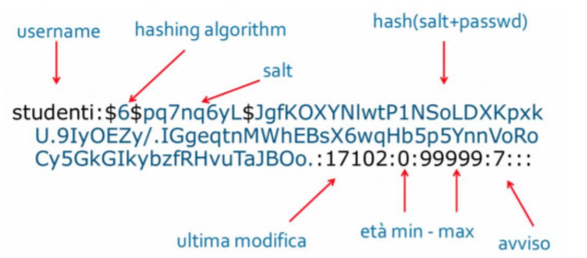
\includegraphics[scale=.9]{img/34.PNG}
			\end{center}
		\end{framed}
	\end{itemize}
	\item Attenzione alle variabili \emph{alfa} e \emph{beta}, che non solo sono presenti, ma anche globali (quindi vanno dichiarate).
	\begin{verbatim}
		.data
		alfa: .long 0
		beta: .long 0
	\end{verbatim}
	\item Chiamo la leggiint e sposto in \emph{alfa} il risultato, che sappiamo essere nel registro rax
	\begin{verbatim}
		call leggiint
		mov %eax, alfa(%rip)
	\end{verbatim}
	\item Stessa cosa con \emph{beta}
	\begin{verbatim}
		call leggiint
		mov %eax, beta(%rip)
	\end{verbatim}
	\item Metto in rdi il primo argomento e in rsi il secondo. Pongo inoltre il risultato in \emph{ris}
	\begin{verbatim}
		mov alfa(%rip), %edi
		mov beta(%rip), %esi
		call elab1
		mov %eax, -8(%rbp)
	\end{verbatim}
	\item Eseguo la scriviint ponendo \emph{ris} nel registro edi (secondo lo standard)
	\begin{verbatim}
		mov -8(%rbp), %edi
		CALL scriviint
	\end{verbatim}
	\item La funzione \emph{main} restituisce $0$ se tutto è andato per il verso giusto (un numero diverso da zero consiste nell'identificativo di un errore). Per restituire $0$ utilizziamo l'istruzione XOR sul registro EAX (RAX, bastano 32 bit visto che si restituisce un \emph{int})
	\begin{verbatim}
		xorl %eax, %eax
	\end{verbatim}
	\item Concludiamo sbarazzandoci del prologo e restituendo il controllo
	\begin{verbatim}
		leave
		ret
	\end{verbatim}
\end{itemize}
\paragraph{Osservazione} Possiamo includere in un file assembler servi.cpp?
\begin{verbatim}
	#include "servi.cpp"
\end{verbatim}
Il compilatore si lamenta (\emph{junk}). Non ha senso includere un file di un certo linguaggio in uno con un altro linguaggio. 
\paragraph{Ottimizzazione} 
L'ottimizzazione non si ottiene dalla riduzione del numero di istruzioni, ma da altre cose: scelta di istruzioni accurate, scritture in memoria solo quando necessario.

\subsubsection{Passaggio di parametri per riferimento (pag.41)}
Proviamo a fare una versione simile dell'esercizio precedente, ma con la presenza di un tipo di riferimento.
\begin{framed}
	\noindent \textbf{Codice c++}
	\begin{verbatim}
		// programma sommmaintRif, file es3a.cpp
		#include"servi.cpp"
		extern "C" void elab3(int& tot, int n1, int n2);
		int main() { 
			int a, b; int ris; <-------- a frosini e' sfuggita una &
			a = leggiint();
			b = leggiint();
			elab3(ris, a, b);
			scriviint(ris);
			nuovalinea();
		};
		// programma sommmaintRif, file es1b.cpp
		extern "C" int elab3(int& tot, int n1, int n2) { 
			int i, j;
			i = n1+n2;
			j = n1-n2;
			tot = i*j;
		};
	\end{verbatim}
\end{framed}
\paragraph{Traduzione Assembler di elab3}
\begin{verbatim}
	.text
	.global elab3
	elab3:
	push %rbp
	mov %rsp, %rbp
	sub $32, %rsp
	
	# copia tot al suo posto
	mov %rdi, -8(%rbp)
	
	# copia n1 ed n2 al suo posto
	mov %esi, -16(%rbp)
	mov %edx, -12(%rbp)
	
	# i = n1 + n2
	mov -16(%rbp), %eax
	add -12(%rbp), %eax
	mov %eax, -24(%rbp)
	
	# j = n1 - n2
	mov -16(%rbp), %eax
	add -12(%rbp), %ecx
	sub %eax, %ecx
	mov %ecx, -20(%rbp)
	
	# tot = i*j
	mov -24(%rbp), %eax
	imull -20(%rbp), %eax
	
	mov -8(%rbp), %rdx
	mov %eax, (%rdx)
	
	leave
	ret
\end{verbatim}

\begin{center}
	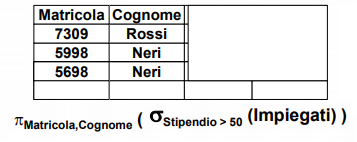
\includegraphics{img/35.PNG}
\end{center}
\begin{itemize}
	\item Pongo il vecchio rbp nella pila, aggiorno il valore di rbp e riservo 32 byte (32 invece di 24 per rispettare rsp multiplo di 16)
	\begin{verbatim}
		push %rbp
		mov %rsp, %rbp
		sub $32, %rsp
	\end{verbatim}
	\item Copio \emph{tot}, così come tutte le altre variabili (secondo lo standard) $n1$ ed $n2$.
	\begin{verbatim}
		mov %rdi, -8(%rbp)
		mov %esi, -16(%rbp)
		mov %edx, -12(%rbp)
	\end{verbatim}
	\item Sulla somma e sulla differenza non ci sono differenze importanti rispetto all'esercizio precedente.
	\item Recupero $i$ ponendolo in eax. Teniamo conto che in \&tot ci sarà l'indirizzo della variabile: sposto il contenuto della parte in un registro sporcabile, utilizzo l'indirizzamento indiretto per aggiornare il contenuto dell'indirizzo posto in rdx.
	\begin{verbatim}
		mov -24(%rbp), %eax
		imull -20(%rbp), %eax
		
		mov -8(%rbp), %rdx
		mov %eax, (%rdx)
	\end{verbatim}
	\item La funzione non restituisce niente, quindi mi limito a terminarla con \emph{leave} e \emph{ret}.
	\begin{verbatim}
		leave
		ret
	\end{verbatim}
\end{itemize}
\paragraph{Traduciamo anche il main}
\begin{verbatim}
	.text
	.global main
	main:
	push %rbp
	mov %rsp, %rbp
	
	call leggiint
	mov %eax, -8(%rbp)
	
	call leggiint
	mov %eax, -4(%rbp)   
	
	lea -16(%rbp), %rdi
	mov -8(%rbp), %esi
	mov -4(%rbp), %edx
	call elab3
	
	.Lnext:     
	mov -16(%rbp), %edi
	call scriviint
	call nuovalinea
	leave 
	ret
\end{verbatim}
\begin{center}
	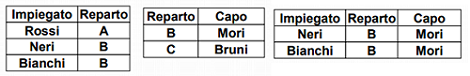
\includegraphics{img/36.PNG}
\end{center}
\begin{itemize}
	\item Pongo il vecchio rbp nella pila, aggiorno il valore di rbp e riservo un certo numero di byte per \emph{b}, \emph{a} e \emph{ris}.
	\item Le chiamate di leggiint non sono tanto diverse rispetto all'esercizio precedente
	\item Sposto nel registro rdi l'indirizzo della variabile \emph{tot} usando la LEA. Sistemo anche le variabili $n1$ e $n2$.
	\begin{verbatim}
		lea -16(%rbp), %rdi 
		mov -8(%rbp), %esi
		mov -4(%rbp), %edx
		call elab3
	\end{verbatim}
	\item Eseguo le funzioni rimanenti all'interno del \emph{main}, nulla di particolare da segnalare.
\end{itemize}
\subsubsection{Passaggio di parametro array (pag.50)}
\begin{framed}
	\noindent \textbf{Codice c++} 
	\begin{multicols}{2}
		\begin{verbatim}
			// programma array, file es6a.cpp
			#include "servi.cpp"
			extern "C" void raddoppia(int a[], int n);
			int main() {
				int ar[5];
				int i;
				for(i = 0; i < 5; i++)
				ar[i] = leggiint();
				raddoppia(ar, 5);
				for(i = 0; i < 5; i++)
				scriviint(ar[i]);
				nuovalinea();
			}
		\end{verbatim}
		\columnbreak
		\begin{verbatim}
			// programma array, file es6b.cpp
			extern "C" void raddoppia(int a[], int n){
				int i;
				for(i = 0; i < n; i++)
				a[i] = 2*a[i]; 
			}
		\end{verbatim}
	\end{multicols}
\end{framed}
\clearpage 
\paragraph{Traduzione assembler di raddoppia}
\begin{verbatim}
	.text
	.global raddoppia
	raddoppia: 
	push %rbp
	mov %rsp, %rbp
	sub $16, %rsp
	
	mov %rdi, -8(%rbp)
	mov %esi, -16(%rbp)
	
	# inizializzazione (i = 0)
	mov $0, -12(%rbp)
	.Lfor:     # Verifica della condizione (i < n)
	cmp %esi, -12(%rbp)
	jl .Lcorpo
	jmp .Lfine
	.Lcorpo:     
	# caricare %rdx
	movslq -12(%rbp), %rdx
	
	mov (%rdi, %rdx, 4), %eax
	sal $1, %eax <--- (stesso OPCODE di SHL)
	mov %eax, (%rdi, %rdx, 4)
	
	# i++
	incl -12(%rbp)
	jmp .Lfor
	.Lfine:      leave
	ret
\end{verbatim}

\begin{center}
	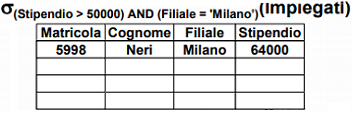
\includegraphics[scale=.9]{img/32.PNG}
\end{center} 
\begin{itemize}
	\item Pongo il vecchio rbp nella pila, aggiorno il valore di rbp e riservo un certo numero di byte per \emph{a}, \emph{n} ed \emph{i}.
	\begin{verbatim}
		push %rbp
		mov %rsp, %rbp
		sub $16, %rsp
	\end{verbatim}
	\item Pongo i valori degli argomenti in memoria
	\begin{verbatim}
		mov %rdi, -8(%rbp)
		mov %esi, -16(%rbp)
	\end{verbatim}
	per quanto riguarda l'array \emph{a} ricordiamoci che poniamo in memoria l'indirizzo del primo elemento dell'array. Ricordarsi che il primo elemento sta per forza negli indirizzi più bassi.
	\item Novità rispetto agli esercizi precedenti è l'introduzione di un for. Ricordiamo, a tal proposito, le spiegazioni sui cicli dalle dispense di Stea. In particolare, dobbiamo ricordare l'ordine delle operazioni in un for
	\begin{enumerate}
		\item inizializzazione del counter;
		\begin{verbatim}
			mov $0, -12(%rbp)
		\end{verbatim}
		\item verifica della validità della condizione;
		\item esecuzione del corpo del for (vedere dopo);
		\item ritorno al secondo punto.
		\begin{verbatim}
			jmp .Lfor
		\end{verbatim}
	\end{enumerate}
	\begin{framed}
		\item Dobbiamo caricare il registro rdx col valore del contatore, in modo da poterlo utilizzare per prendere l'elemento dell'array
		\begin{verbatim}
			movslq -12(%rbp), %rdx
		\end{verbatim}
		con questa istruzione teniamo conto del segno nel passaggio da \emph{long} a \emph{quad} (se utilizzo solo la MOV emergono problemi con un numero elevato di iterazioni). perché dobbiamo dire questo? \textbf{Nell'indirizzamento coi registri dobbiamo utilizzare registri a 64 bit} (il compilatore fa storie in caso contrario), tuttavia
		\begin{itemize}
			\item \textbf{il numero coinvolto nello spostamento è un numero a 32 bit},
			\item ed è anche intero.
		\end{itemize}
		Segue che \textbf{l'estensione di campo non è quella dei naturali} (in quel caso mi sarebbe bastato una semplice MOV con registri a 32 bit, considerato che i bit più significativi vengono azzerati)
	\end{framed}
	\item Sposto nel registro eax il valore da moltiplicare per due. Il prodotto è per una potenza della base due, quindi posso fare la cosa con uno shift a sinistra. Concludo riportando il numero shiftato in memoria.
	\begin{verbatim}
		mov (%rdi, %rdx, 4), %eax
		sal $1, %eax <--- va bene anche shl (stesso opcode)
		mov %eax, (%rdi, %rdx, 4)
	\end{verbatim}
	per quanto riguarda l'indirizzamento bimodificato
	\[\text{Indirizzo}=\left|\text{rdi}+\text{rdx}\times\text{4}\right|_{\text{modulo}_{2^{64}}}\]
	rdi è il registro avente per contenuto l'indirizzo del primo elemento dell'array (primo argomento della funzione), rdx è il registro dove poniamo ogni volta il contenuto della variabile contatore. Sapendo che ogni intero occupa 4 byte si capisce al volo che incrementando rdx passeremo all'elemento immediatamente successivo dell'array.
\end{itemize}
\paragraph{Traduciamo anche il main}
\begin{verbatim}
	.set ar, -24
	.set i, -32
	
	.text
	.global main
	main:
	push %rbp
	mov %rsp, %rbp
	sub $32, %rsp
	
	movl $0, i(%rbp) # <---- i = 0
	.Lfor1:        cmp $5, i(%rbp), 
	jl .Lcorpo1 # <--- i < 5
	jmp .Lfine1
	.Lcorpo1:
	call leggiint
	movslq i(%rbp), %rcx
	mov %eax, ar(%rbp, %rcx, 4)
	incl i(%rbp)
	jmp .Lfor1 # ritorno alla condizione 
	.Lfine1:       lea -24(%rbp), %rdi
	mov $5, %esi
	call raddoppia
	
	movl $0, i(%rbp)
	.Lfor2:
	cmp $5, i(%rbp)
	jl .Lcorpo2
	jmp .Lfine2
	.Lcorpo2:
	movslq i(%rbp), %rcx
	mov ar(%rbp, %rcx, 4), %rdi
	call scriviint
	incl i(%rbp)
	jmp .Lfor2
	.Lfine2:
	call nuovalinea
	
	leave
	ret
\end{verbatim}
\begin{center}
	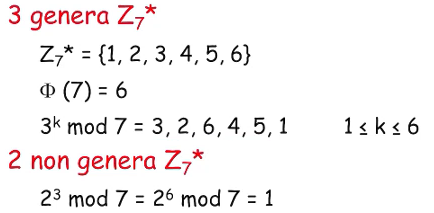
\includegraphics[scale=.9]{img/23.PNG}
\end{center} 
\begin{itemize}
	\item Nella creazione dell'array trattiamo ogni elemento come se fosse un qualcosa di indipendente. Li poniamo in modo tale che l'allineamento sia rispettato. Un modo per ricordarsi che l'array deve essere posto in un certo modo sono le istruzioni per visitare, in un ciclo, tutti gli elementi dell'array (somma sul puntatore ad array): se poniamo in fondo alla pila (negli indirizzi più alti) il primo elemento allora il meccanismo non funziona.
	\begin{framed}
		\item \textbf{Direttive \emph{set}}. Con le direttive \emph{set} andiamo a creare delle costanti (già visto a Reti logiche, ricordarsi \emph{pippo} e la domanda del pretest).
		\begin{verbatim}
			.set ar, -24
			.set i, -32
		\end{verbatim} Possiamo assegnare SOLO delle costanti, non stiamo lavorando con delle macro. 
		\begin{verbatim}
			.set i, -32(%rbp) <------- SBAGLIATO!
		\end{verbatim}
	\end{framed}
	\item Come al solito memorizziamo il vecchio rbp e allochiamo lo spazio necessario
	\begin{verbatim}
		push %rbp
		mov %rsp, %rbp
		sub $32, %rsp
	\end{verbatim}
	\item Poniamo in rdi l'indirizzo dell'array, che è l'indirizzo del primo elemento dell'array.
	\begin{verbatim}
		lea -24(%rbp), %rdi
	\end{verbatim}
	non si utilizzi la mov invece della lea
	\begin{verbatim}
		mov -24(%rbp), %rdi
	\end{verbatim}
	che sposta in memoria il contenuto del primo elemento dell'array, E NON L'INDIRIZZO DELLO STESSO!
	\item Poniamo anche il secondo argomento e chiamiamo la funzione \emph{raddoppia}
	\begin{verbatim}
		mov $5, %esi
		call raddoppia
	\end{verbatim}
	\item Il for per la stampa dell'array (legata alla funzione \emph{scriviint}) non è strutturato in modo diverso dal primo.
	\begin{framed}
		\item \textbf{Osservazione sui registri \emph{scratch}}: Uno studente si è accorto di un errore del prof nell'uso del registro rcx. Il codice inizialmente era così
		\begin{verbatim}
			movslq i(%rbp), %rcx
			call leggiint
			mov %eax, ar(%rbp, %rcx, 4)
		\end{verbatim}
		La cosa è un problema: rcx, essendo scratch, potrebbe non essere preservato nella funzione \emph{leggiint}. Se proviamo ad eseguire otterremo un \emph{Bus error}: questo perché la modifica dell'rcx da parte di \emph{leggiint} ci porta nel cosiddetto \emph{buco della memoria} (la parte di memoria non utilizzata introdotta nelle lezioni precedenti). Abbiamo due soluzioni possibili:
		\begin{itemize}
			\item scegliere un registro \emph{non scratch}
			\item invertire le prime due righe della parte incriminata (soluzione adottata dal prof per questo caso)
		\end{itemize}
	\end{framed}
\end{itemize}

\subsubsection{Passaggio di parametro struttura (pag.64)}
\begin{framed}
	\noindent \textbf{Codice c++} 
	\begin{multicols}{2}
		\begin{verbatim}
			// programma struttura, file es10a.cpp
			#include "servi.cpp"
			struct s  { int n1; char c; int n2; };
			extern "C" s leggis() {
				s ss;
				ss.n1 = leggiint();
				ss.c = leggichar();
				ss.n2 = leggiint();
				return ss; 
			}
			extern "C" void scrivis(s ss) {
				scriviint(ss.n1);
				scrivichar(ss.c);
				scriviint(ss.n2);
				nuovalinea();
			}
			
			extern "C" s fai(s st);
			int main() {
				s st1, st2;
				st1 = leggis();
				st2 = fai(st1);
				scrivis(st2);
				return 0;
			}
			
			// programma struttura, file es10b.cpp
			struct s { int n1; char c; int n2; };
			extern "C" s fai(s st) {
				s ss;
				ss.n1 = st.n1 + 5;
				ss.c = st.c + 1;
				ss.n2 = st.n2 + 10;
				return ss;
			}
		\end{verbatim}
	\end{multicols}
\end{framed}

\noindent \textbf{Traduzione assembler di es10b}
\begin{verbatim}
	.text
	.global fai
	fai:
	push %rbp
	mov %rsp, %rbp
	sub $32, %rsp
	mov %rdi, -16(%rbp)
	mov %esi, -8(%rbp)
	
	# ss.n1 = st.n1 + 5
	mov -16(%rbp), %eax
	add $5, %eax
	mov %eax, -32(%rbp)
	# ss.c = st.c + 1
	mov -12(%rbp), %al
	add $1, %al
	mov %al, -28(%rbp)
	# ss.n2 = st.n1 + 10
	mov -8(%rbp), %eax
	add $10, %eax
	mov %eax, -24(%rbp)
	# return ss
	mov -32(%rbp), %rax
	mov -24(%rbp), %edx
	
	leave
	ret
\end{verbatim}
\begin{center}
	\includegraphics[scale=.9]{img/31.PNG}
\end{center} 
\begin{itemize}
	\item Nel riservare lo spazio agli elementi della struttura ricordiamo lo stesso ragionamento visto per gli array: se io incremento devo passare all'elemento successivo. Segue che \textbf{in cima alla pila (indirizzi più bassi) ci saranno i primi elementi della struttura}.
	
	\item Memorizziamo l'rbp vecchio e riserviamo lo spazio di memoria necessario, in luce delle considerazioni precedenti
	\begin{verbatim}
		push %rbp
		mov %rsp, %rbp
		sub $32, %rsp
	\end{verbatim}
	\item Sistemiamo la struttura posta in ingresso come parametro. Abbiamo 16byte divisi in due blocchi, seguono due operazioni di mov. Si consideri che finchè il parametro sta in 16byte non è un problema. Segue
	\begin{verbatim}
		mov %rdi, -16(%rbp)
		mov %esi, -8(%rbp)
	\end{verbatim}
	\textbf{Nel primo registro vanno i primi elementi della struttura, i rimanenti nel secondo registro.}
	\item Per le operazioni di somma
	\begin{itemize}
		\item spostiamo l'operando non costante dalla memoria a un registro
		\item eseguiamo l'addizione su quel registro
		\item spostiamo il contenuto modificato nella variabile indicata nell'assegnamento
	\end{itemize}
	segue
	\small
	\begin{verbatim}
		# ss.n1 = st.n1 + 5
		mov -16(%rbp), %eax # <------------ sposto st.n1 in eax
		add $5, %eax # <----- sommo 5 ad eax
		mov %eax, -32(%rbp) # <--- sposto il contenuto addizionato in ss.n1
		
		# ss.c = st.c + 1
		mov -12(%rbp), %al # <---- sposto st.c in al
		add $1, %al # <------- sommo 1 ad al
		mov %al, -28(%rbp) # <---- sposto il contenuto incrementato in ss.c
		
		# ss.n2 = st.n1 + 10
		mov -8(%rbp), %eax # <---- sposto st.n1 in eax
		add $10, %eax # <----- sommo 10 ad eax
		mov %eax, -24(%rbp) # <----- sposto il contenuto addizionato in ss.n2
	\end{verbatim}
	\item La struttura è di 16byte, divisa in due blocchi. Dobbiamo eseguire due spostamenti di memoria per la struttura restituita dalla funzione 
	\begin{verbatim}
		mov -32(%rbp), %rax
		mov -24(%rbp), %edx
	\end{verbatim}
	Come parte meno significativa poniamo la prima riga della struttura (quella a indirizzo più basso, col primo intero e il char), l'altra come parte più significativa (quella col secondo intero).
	\item Chiudiamo come al solito
	\begin{verbatim}
		leave
		ret
	\end{verbatim}
	\begin{framed}
		\item \textbf{Osservazione sulla dichiarazione delle strutture}.
		\begin{verbatim}
			struct s  { int n1; char c; int n2; };
		\end{verbatim}
		Ricordiamoci che il compilatore lavora singolarmente su ogni file. 
		\begin{itemize}
			\item Nel file col main abbiamo la dichiarazione della struttura \emph{s} (la utilizziamo nel main, è fondamentale perché il compilatore deve sapere quanto spazio allocare per la struttura - non tanto per gli elementi interni)
			\item Nel file con la funzione \emph{fai} si potrebbe pensare che non è necessario definire la struttura \emph{s}: FALSO, altrimenti il compilatore non potrà conoscere gli offset della struttura (la funzione \emph{fai} lavora su singoli elementi delle strutture)
		\end{itemize}
	\end{framed}
	\item \textbf{Proviamo a cambiare la struttura \emph{s} in uno dei due files: se ne accorge qualcuno?}
	
	Il compilatore no, visto che lavora sui singoli files. Il collegatore vede tutto insieme, ma non si preoccupa di queste cose. Quindi, se siamo fortunati, non se ne accorge nessuno. Se modifico la definizione nel primo file non è un problema: sposto gli elementi ma la dimensione complessiva della struttura è la stessa. Nel secondo file, invece, la cosa genera problemi: non vengono segnalati errori, ma il risultato ottenuto non è quello desiderato.
\end{itemize}
\paragraph{Traduzione assembler del main}
\begin{center}
	\includegraphics{img/37.PNG}
\end{center} 
\begin{verbatim}
	.text
	.global main
	main:
	push %rbp
	mov %rsp, %rbp
	
	call leggis
	mov %rax, -16(%rbp)
	mov %edx, -8(%rbp) # <---- memorizzo la struttura restituita in st1
	
	mov -16(%rbp), %rdi
	mov -8(%rbp), %edx # <--- pongo la struttura st1 come argomento della funzione fai
	call fai
	mov %rax, -32(%rbp)
	mov %edx, -24(%rbp) # <--- memorizzo la struttura restituita in st2
	
	mov -32(%rbp), %rdi
	mov -24(%rbp), %esi # <--- pongo la struttura st2 come argomento della funzione scrivis
	call scrivis
	
	xorl %eax, %eax # <--- restituisco 0
	leave
	ret # <---- concludo come al solito
\end{verbatim}
\endgroup
	\chapter{Venerdì 19/03/2021}

\section{Traduzione dei nomi da C++ ad Assembler}
\paragraph{Cosa abbiamo visto fino ad ora?} Fino ad ora abbiamo affrontato questioni valide sia per il C che per il C++.
\paragraph{Overloading in C} Fino ad ora abbiamo introdotto le funzioni in questo modo
\begin{verbatim}
	extern "C" elab(...)
\end{verbatim}
indicare \emph{C} significa dire che la funzione rispetta lo standard del C. Nel C, ricordiamo, non è presente l'overloading e i nomi delle funzioni vengono tradotti esattamente come indicati nel codice.
\paragraph{Overloading in C++} L'overloading è presente in C++ e deve essere trattato. Possiamo avere funzioni con lo stesso nome, ma parametri in ingresso diversi (sia nel numero che nei tipi).
\begin{verbatim}
	elab(int)
	elab(int, int)
	elab(miastruct)
	elab(int*)
\end{verbatim}
queste sono funzioni diverse! Il compilatore, quando vede una chiamata del tipo
\begin{verbatim}
	elab(5)
\end{verbatim}
deve capire quale funzione chiamare. Ricordiamoci che due funzioni non si distinguono per il valore restituito: segue che non posso avere funzioni del tipo
\begin{verbatim}
	char elab(int)
	int elab(int)
\end{verbatim}
Se il compilatore sta compilando un file e nello stesso è presente la definizione di ciascuna di queste funzioni la cosa è semplice, mentre diventa più complessa se alcune funzioni (o tutte le funzioni) sono definite in altri files. Non posso indicare l'indirizzo della funzione, visto che non lo conosco: lascerò al collegatore le informazioni necessarie per capire quale funzione ci interessa. Il collegatore guarderà le tabelle dei simboli di tutti i files. 
\paragraph{In base a cosa stabilisco se l'etichetta è la stessa che sto cercando?} L'etichetta è una stringa, quindi mediante corrispondenza tra stringhe. 
\paragraph{Problema} Non posso definire più funzioni con la stessa etichetta \emph{elab}. Il collegatore vedrebbe più definizioni della stessa etichetta. Il problema nasce perché vogliamo utilizzare lo stesso collegatore del C.
\paragraph{Soluzione}  Modifichiamo i nomi posti delle etichette codificando all'interno gli argomenti della funzione. Dobbiamo individuare un algoritmo che produce la stessa stringa data la stessa funzione (ricordiamoci che il compilatore agisce sui singoli files in modo distinto).

\subsection{Regole per le etichette delle funzioni}
\paragraph{Osservazione} L'algoritmo non è standard. Esistono compilatori diversi con regole diverse.
\paragraph{Regole} Prendiamo una funzione
\begin{verbatim}
	funz(tipo1, tipo2, ..., tipoN)
\end{verbatim}
\begin{enumerate}
	\item La stringa inizia sempre così
	\begin{verbatim}
		_Z
	\end{verbatim}
	\item Segue il nome della funzione, preceduto dal numero di caratteri del nome (devo sapere quando si inizia a parlare dei tipi nella stringa)
	\begin{verbatim}
		4funz
	\end{verbatim}
	\item Segue la traduzione di ognuno dei tipi
	\begin{verbatim}
		_Z4funzS1S2...SN
	\end{verbatim}
\end{enumerate}
\paragraph{Quali sono i possibili tipi nel C++?} Il numero di tipi è piuttosto alto: abbiamo 
\begin{itemize}
	\item i tipi base (char, bool, int, long, unsigned/signed ....)
	\item i tipi definiti dall'utente (enum, class, struct...)
	\item i tipi composti (*,\&, const, array...)
\end{itemize}
\subsubsection{Tipi base} Per ogni tipo base c'è una lettera identificativa
\begin{center}
	\includegraphics[scale=0.70]{img/38.PNG}
\end{center}  
notare che in assenza di argomenti è presente la lettera \emph{v} (\emph{void}). In presenza di più argomenti relativi a tipi base si pongono più caratteri in sequenza
\begin{verbatim}
	funz() ---> _Z4funzx
	funz(int) --->_Z4funzi
	funz(long int) ---> _Z4funzl
	funz(short int) ---> _Z4funzs
	funz(int, int) ---> _Z4funzii
\end{verbatim}
\subsubsection{Struttura} Supponiamo di voler trovare la stringa relativa a questa funzione
\begin{verbatim}
	funz(miastrutt)
\end{verbatim}
Trattiamo la cosa in modo simile al nome della funzione. \emph{miastrutt} ha nove caratteri, quindi
\begin{verbatim}
	_Z4funz9miastrutt
\end{verbatim}
Vediamo un ulteriore esempio che combina una struttura e un tipo base
\begin{verbatim}
	funz(mias, int, char)  ----> _Z4funz4miasic
\end{verbatim}
\subsubsection{Puntatori}
Poniamo P seguito dal tipo
\begin{verbatim}
	tipo* ----> PStipo
\end{verbatim}
Vediamo alcuni esempi
\begin{verbatim}
	int* ---> Pi
	mias* ---> P4mias
	int** --->  PPi
\end{verbatim}
\subsubsection{Riferimenti}
Poniamo R seguito dal tipo 
\begin{verbatim}
	tipo& ---> RStipo
\end{verbatim}
Vediamo alcuni esempi
\begin{verbatim}
	int& ---> Ri
	mias*& ---> RP4mias
\end{verbatim}
\subsubsection{Costanti}
Sulle costanti dobbiamo fermarci un attimo
\begin{verbatim}
	(1) const int*
	(2) int const* ---> Pki
	(3) int* const 
\end{verbatim}
Quanti tipi diversi ho dichiarato? Due:
\begin{itemize}
	\item Puntatore a intero costante (1 e 2, posso modificare l'indirizzo puntato ma non il valore dell'intero puntato)
	\item Puntatore costante a intero (3, posso modificare il valore dell'intero ma non l'indirizzo puntato)
\end{itemize}
\emph{const} si traduce con una K maiuscola. Nel capire di quale puntatore stiamo parlando dobbiamo ricordarci che \textbf{il \emph{const} fa sempre riferimento a ciò che è prima, tranne quando è in cima (in quel caso fa riferimento a ciò che viene dopo)}.
\paragraph{Regola della spirale} La regola della spirale (suggerimento mio, non di Lettieri) permette di capire in modo più facile di quale puntatore stiamo parlando:
\begin{itemize}
	\item parto dal nome dell'elemento;
	\item mi sposto indietro facendo un giro in senso orario (se becco la keyword \emph{const} devo contare fino a tre, e guardare a chi fa riferimento \underline{usando la regola di prima});
	\item ripeto fino al termine dell'espressione.
\end{itemize}
\begin{center}
	\includegraphics[scale=0.80]{img/154.PNG}
\end{center}  

\paragraph{Confronto tra tipi e tipi costanti nei parametri} Attenzione alle seguenti funzioni
\begin{verbatim}
	funz(int)
	funz(const int)
\end{verbatim}
non sono due funzioni diverse. Entrambe generano come stringa \begin{verbatim}_Z4funzi\end{verbatim}Nel secondo caso dico che non posso modificare la cosa che mi viene passata, ma succede la stessa cosa anche nel primo caso visto che si ha un passaggio per valore. Il ragionamento è valido anche parlando in modo generico.\paragraph{Conseguenza} In \emph{KPi} la lettera K non dice sostanzialmente niente, può essere tolto.
\[\boxed{\text{Se nel costruire l'etichetta pongo un \emph{K} all'inizio allora possiamo toglierlo}}\]
\subsubsection{Array}
Prendiamo i seguenti esempi
\begin{verbatim}
	f(int a[10])
	f(int a[100])     -------------> _Z1fPi
	f(int a[])
\end{verbatim}
sono le stesse funzioni, il numero non entra a far parte del nome della funzione. Inoltre, la seguente funzione è uguale alle precedenti
\begin{verbatim}
	f(int* a)          -------------> _Z1fPi
\end{verbatim}
Ricordiamo che passare un array come parametro significa passare un puntatore al primo elemento dell'array. Il fatto che un array decada in puntatore è una delle cose più criticate del C, conseguentemente anche del C++.\begin{framed}\noindent \textbf{Osservazione}: non affronteremo la regola per scrivere le etichette a riguardo, ma dobbiamo tenere a mente che funzioni di questo tipo non sono equivalenti
	\begin{verbatim}
		f(int a[][10])
		f(int a[][20])
	\end{verbatim} 
	possiamo mantenere implicita solo la prima dimensione, quella successiva no. Devo conoscere quanti interi sono presenti in ogni elemento dell'array, altrimenti non saprei come raggiungerli. Raggiungo l'elemento $a[i][j]$ con la seguente formula
	\begin{verbatim}
		i*secondaDim+j
	\end{verbatim}
\end{framed}

\subsubsection{Esempi di etichette con costanti}
\begin{itemize}
	\item Per ogni esempio
	\begin{itemize}
		\item Metto il solito inizio
		\item Per il nome pongo \emph{1f}
	\end{itemize}
	\item \begin{verbatim}
		f(int const*)   ----->  _Z1fPKi
	\end{verbatim}
	\begin{itemize}
		\item Per il tipo pongo \emph{PKi}: abbiamo un puntatore a un intero costante
	\end{itemize}
	\item \begin{verbatim}
		f(const int*)   ----->  _Z1fPKi
	\end{verbatim}
	\begin{itemize}
		\item Ricordiamoci la regola detta prima. L'etichetta ottenuta è la stessa della funzione precedente
	\end{itemize}
	\item \begin{verbatim}
		f(int* const)   ----->  _Z1fKPi   ----->  _Z1fPi
	\end{verbatim}
	\begin{itemize}
		\item Per il tipo pongo \emph{Pi}: abbiamo un puntatore costante a intero, abbiamo già detto che non ha senso mettere prima \emph{K}
	\end{itemize}
	\item \begin{verbatim}
		f(int const* const)   ----->  _Z1fKPKi   ----->  _Z1fPKi
	\end{verbatim}
	\begin{itemize}
		\item Per il tipo pongo \emph{PKi}: abbiamo un puntatore costante a intero costante. La \emph{K} prima non ha senso, quella dopo P invece è necessaria.
	\end{itemize}
	\item \begin{verbatim}
		f(int* const*)   ----->  _Z1fPKPi
	\end{verbatim}
	\begin{itemize}
		\item Per il tipo pongo \emph{PKPi}: abbiamo un puntatore a puntatore costante di intero.
	\end{itemize}
	\item \begin{verbatim}
		f(int*)   ----->  _Z1fPi
	\end{verbatim}
	\begin{itemize}
		\item Per il tipo pongo \emph{Pi}: abbiamo un puntatore a intero
	\end{itemize}
\end{itemize}
\begin{center}
	\includegraphics[scale=0.80]{img/155.PNG}
\end{center} 

\begin{framed}\noindent \textbf{Curiosità sui puntatori}. L'elemento $a[i]$ viene tradotto nel seguente modo
	\begin{verbatim}
		*(a+i)
	\end{verbatim}
	questa cosa è talmente vera in C, e quindi in C++, che possiamo dire
	\begin{verbatim}
		*(i+a)
	\end{verbatim}
	segue che dire
	\begin{verbatim}
		i[a]
	\end{verbatim}
	equivale a dire $a[i]$. La notazione è utilizzabile senza alcun problema in C e in C++.\end{framed}

	
\chapter{Lunedì 22/03/2021}
\section{Corrispondenza C++-Assembler: classi}
\begin{verbatim}
	class c {
		int i;
		long j;
		....
		c();
		c(int);
		~c();
	};
\end{verbatim}
Parliamo di classi: esse permettono di raggruppare insieme dati e codice, definire un nuovo tipo (astratto) e la sua rappresentazione interna (sottotipi), definire quali operazioni è possibile eseguire su questo sottotipo.
Possiamo definire \emph{funzioni membro}, distinguere la visibilità dei vari elementi definiti in una classe, definire funzioni particolari come costruttori (anche più di uno in base ai tipi) e i distruttori.
\subsection{Prima implementazione (da C++ a C): compilatore \emph{cfront}} La prima implementazione è avvenuta con un compilatore chiamato \emph{cfront} in cui si passa da C++ a C. Il linguaggio verso cui si traduce non deve essere per forza a basso livello.
\paragraph{Come traduciamo una chiamata di funzione membro?} Prendiamo il seguente codice
\begin{verbatim}
	int main() {
		c miac;
		miac.f(...);
	}
\end{verbatim}
\begin{itemize}
	\item Il compilatore osserva la definizione della classe: questa non produce di per se alcun codice, ma determina una struttura dati interna al compilatore. Il compilatore saprà che esiste una struttura dati che presenta certi dati e certe funzioni membro, con costruttore e distruttore.
	\item Quando vede dichiarata un'istanza di quell'oggetto il compilatore si preoccupa di allocare spazio per quell'istanza.
	\item Quando vede un'invocazione della funzione membro di un oggetto verifica che la si possa chiamare in quel punto (elemento public o no?). Solo dopo questo step traduce la chiamata.
\end{itemize}

\paragraph{Allocazione dell'oggetto} Lo spazio allocato per l'oggetto è lo spazio delle sue variabili membro. La sua parte dati viene tradotta in uno struct:
\begin{verbatim}
	struct c {
		int i;
		long j;
	};
\end{verbatim}
Le funzioni membro diventano funzioni globali, definite però all'interno di una classe. I nomi non coincideranno con quelli delle funzioni: due funzioni globali non possono avere stesso nome, significherebbe impedire a due classi diverse di assumere lo stesso nome per una funzione membro.
\paragraph{Argomento implicito nelle funzioni} Le funzioni membro ricevono, in modo implicito, un puntatore all'oggetto su cui devono lavorare
\begin{verbatim}
	void c_f(c* this, ...)
\end{verbatim}
\paragraph{Dereferenziazione} Sappiamo che scrivendo una cosa del genere
\begin{verbatim}
	void c_f(c* this, ...) {
		i = 10;
	}
\end{verbatim}
il compilatore intenderà i come il campo dell'oggetto su cui la funzione membro è stata chiamata. 
\begin{verbatim}
	void c_f(c* this, ...) {
		this->i = 10;
	}
\end{verbatim}
Abbiamo una dereferenziazione implicita (nulla di nuovo rispetto a quanto visto a Fondamenti di programmazione). Segue una traduzione del main di questo tipo
\begin{verbatim}
	int main() {
		c miac;
		c_f(&miac, ...);
	}
\end{verbatim}
\clearpage

\subsection{Implementazione attuale (da C++ ad Assembler direttamente)}
Adesso \emph{cfront} non viene più utilizzato. Abbiamo compilatori che effettuano un passaggio diretto da C++ ad Assembler. Non si hanno grandi differenze concettuali rispetto al \emph{cfront}. 
\paragraph{Cosa dobbiamo sapere?}
\begin{itemize}
	\item Le regole per la traduzione dei nomi delle funzioni membro.
	\item Come viene passato il puntatore \emph{this}.
\end{itemize}

\subsubsection{Traduzione dei nomi delle funzioni membro}
\begin{verbatim}
	class c {
		tipoR funz(tipo1, ..., tipoN)
	}
\end{verbatim}
Il nome della funzione viene tradotto in Assembler nello stesso modo in cui faceva \emph{cfront}. In particolare, il nome della funzione deve contenere il nome della classe. Vediamo le regole:
\begin{itemize}
	\item Si parte con
	\begin{verbatim}
		_Z
	\end{verbatim}
	\item Tutti i caratteri che servono a definire di quale funzione membro stiamo parlando sono posti tra due lettere: N ed E
	\begin{verbatim}
		_ZN    ...       E
	\end{verbatim}
	Indichiamo il nome della classe e il nome della funzione negli stessi modi visti nella scorsa lezione
	\begin{verbatim}
		_ZN1c4funzE
	\end{verbatim}
	Prima il nome della classe, dopo il nome della funzione
	\item Segue la traduzione dei tipi della funzione con i modi già visti, \textbf{SENZA} contare il parametro implicito \emph{this}. Unica differenza: se uno di questi tipi si rifà alla classe associata alla funzione membro il nome della classe non viene ripetuto, ma si pone
	\begin{verbatim}
		S_
	\end{verbatim}
\end{itemize}
\paragraph{Esempio} Vediamo un esempio con la seguente classe
\begin{verbatim}
	class miac {
		void funz1(); <---- _ZN4miac5funzEv
		void funz2(int); <---- _ZN4miac5funzEi
		void funz2(miac*) <---- _ZN4miac5funzEPS_
	}
\end{verbatim}
La regola è un po' più complicata ma ci limiteremo a questo. Il compilatore cerca di ridurre al minimo le ridondanze, per evitare problemi relativi alla lunghezza delle stringhe nel collegatore.
\paragraph{Costruttori} I costruttori si indicano col seguente nome
\begin{verbatim}
	C1
\end{verbatim}
La cosa non è fonte di equivoci: tutti i nomi definiti da un utente iniziano sempre con un numero.
\paragraph{Distruttori} I distruttori si indicano in modo simile
\begin{verbatim}
	D1
\end{verbatim}

\section{Esercizio dalle diapositive di Frosini}
\begingroup
\small
\subsection{Primo esercizio}
\begin{framed}
	\noindent \textbf{Codice C++}
	\begin{verbatim}
		// programma classe1, file clai1.cpp
	\end{verbatim}
	\begin{multicols}{2}
		\begin{verbatim}
			#include "servi.cpp"
			class clai { 
				int ix, iy, iz;
				public:
				clai();
				clai(int, int, int);
				// ...
				void stampa();
				clai somma(int, int, int);
			};
			
			clai::clai() { 
				ix = 0; iy = 0; iz = 0;
			}
			
			clai::clai(int a, int b, int c) { 
				ix = a; iy = b; iz = c;
			}
			
			
			void clai::stampa() { 
				scriviint(ix); 
				scriviint(iy); 
				scriviint(iz);
				nuovalinea();
			}
			
			clai clai::somma(int a, int b, int c) { 
				clai temp;
				temp.ix = ix+a;
				temp.iy = iy+b;
				temp.iz = iz+c;
				
				return temp;
			}
		\end{verbatim}
	\end{multicols}
\end{framed}
\paragraph{Traduzione di \emph{stampa}} 
\begin{verbatim}
	.global  _ZN4clai6stampaEv
	_ZN4clai6stampaEv:
	push %rbp
	mov %rsp, %rbp
	sub $16, %rip
	mov %rdi, -8(%rbp)
	
	mov -8(%rbp), %rax # this
	mov (%rax), %edi # this->ix
	call scriviint
	
	mov -8(%rbp), %rax # this
	mov 4(%rax), %edi # this->iy
	call scriviint
	
	mov -8(%rbp), %rax # this
	mov 8(%rax), %edi # this->iz
	call scriviint
	
	call nuovalinea # Non ho argomenti in ingresso
	
	leave
	ret
\end{verbatim}

\begin{itemize}
	\item \emph{stampa} è una funzione globale che ha in ingresso un solo parametro, quello implicito \emph{this}.
	\item Scriviamo il nome della funzione
	\begin{verbatim}
		_ZN4clai6stampaEv
	\end{verbatim}
	\begin{itemize}
		\item Inizio con i soliti caratteri: \emph{$\_$Z}.
		\item Abbiamo una funzione membro, dunque poniamo nome della classe e nome della funzione membro tra le lettere \emph{N} ed \emph{E}.
		\item Concludo con la lettera \emph{v} (la funzione non presenta parametri in ingresso, \emph{this} non si considera)
	\end{itemize}
	\item Per quanto riguarda il record di attivazione nulla di strano (l'unico elemento da considerare è il parametro \emph{this})
	\begin{center}
		\includegraphics{img/39.PNG}
	\end{center}  
	solito prologo
	\begin{verbatim}
		push %rbp
		mov %rsp, %rbp
		sub $16, %rip
		mov %rdi, -8(%rbp)
	\end{verbatim}
	\item La funzione si limita semplicemente a chiamare quattro funzioni esterne alla classe. I valori posti come parametri di queste funzioni sono sempre dati membro dell'istanza della classe. Segue che dovrò usare il puntatore this per recuperare questi dati, mediante indirizzamento indiretto. 
	\begin{verbatim}
		mov -8(%rbp), %rax # this
		mov (%rax), %edi # this->ix
		call scriviint
		
		mov -8(%rbp), %rax # this
		mov 4(%rax), %edi # this->iy
		call scriviint
		
		mov -8(%rbp), %rax # this
		mov 8(%rax), %edi # this->iz
		call scriviint
		
		call nuovalinea # Non ho argomenti in ingresso
	\end{verbatim}
	\item Concludiamo allo stesso modo con \emph{leave} e \emph{ret}.
\end{itemize}
\paragraph{Traduzione dei costruttori}
I costruttori hanno una sintassi particolare, non restituiscono niente all'apparenza (lo standard suggerisce che siano void). Si adotta una convenzione: la restituzione dell'indirizzo dell'oggetto costruito.
\begin{multicols}{2}
	\begin{verbatim}
		.global _ZN4claiC1Eiii
		_ZN4claiC1Eiii: 
		push %rbp
		mov %rsp, %rbp
		sub $32, %rip
		
		mov %rdi, -8(%rbp)
		# mov %esi, -24(%rbp)
		# mov %edx, -28(%rbp)
		# mov %ecx, -16(%rbp)
		
		mov %esi, (%rdi)
		mov %edx, 4(%rdi)
		mov %ecx, 8(%rdi)
		
		mov %rdi, %rax
		leave
		ret
	\end{verbatim}
	\columnbreak
	\begin{verbatim} 
		.global _ZN4claiC1Ev
		_ZN4claiC1Ev:
		push %rbp
		mov %rsp, %rbp
		sub $16, %rip
		mov %rdi, -8(%rbp)
		
		movl $0, (%rdi)  # this->ix = 0
		movl $0, 4(%rdi)  # this->iy = 0
		movl $0, 8(%rdi)  # this->iz = 0
		
		mov %rdi, %rax
		leave
		ret
	\end{verbatim}
\end{multicols}
\begin{itemize}
	\item \textbf{Primo costruttore (quello senza argomenti)}:
	\begin{itemize}
		\item Scriviamo il nome della funzione
		\begin{verbatim}
			_ZN4claiC1Ev
		\end{verbatim}
		\item Solito prologo per il record di attivazione (stessa struttura vista per la funzione \emph{stampa})
		\begin{verbatim}
			push %rbp
			mov %rsp, %rbp
			sub $16, %rip
			mov %rdi, -8(%rbp)
		\end{verbatim}
		\item Poniamo tutte le variabili della classe uguali a zero, usando un indirizzamento indiretto con displacement
		\begin{verbatim}
			movl $0, (%rdi)  # this->ix = 0
			movl $0, 4(%rdi)  # this->iy = 0
			movl $0, 8(%rdi)  # this->iz = 0
		\end{verbatim}
		\item Restituiamo l'indirizzo dell'oggetto costituito
		\begin{verbatim}
			mov %rdi, %rax
		\end{verbatim}
		\item Concludiamo allo stesso modo
		\begin{verbatim}
			leave
			ret
		\end{verbatim}
	\end{itemize}
	\item \textbf{Secondo costruttore (quello con argomenti)}:
	\begin{itemize}
		\item Scriviamo il nome della funzione
		\begin{verbatim}
			_ZN4claiC1Eiii
		\end{verbatim}
		\item Il record di attivazione conterrà al suo interno anche i parametri in ingresso \emph{a}, \emph{b}, \emph{c}.
		\begin{center}
			\includegraphics{img/40.PNG}
		\end{center}  
		scriviamo il prologo
		\begin{verbatim}
			push %rbp
			mov %rsp, %rbp
			sub $32, %rip
			
			mov %rdi, -8(%rbp)
			mov %esi, -24(%rbp)
			mov %edx, -28(%rbp)
			mov %ecx, -16(%rbp)
		\end{verbatim}
		in aggiunta ad rdi spostiamo anche il contenuto dei parametri in ingresso. 
		\item Aggiorniamo i valori delle variabili. Facciamo la cosa velocemente, passando direttamente i valori dai registri
		\begin{verbatim}
			mov %esi, (%rdi)
			mov %edx, 4(%rdi)
			mov %ecx, 8(%rdi)
		\end{verbatim}
		chiaramente il compilatore, se chiediamo ottimizzazione, farà così e non allocherà quanto allocato prima nel record di attivazione.
		\item Restituiamo l'indirizzo dell'oggetto costituito
		\begin{verbatim}
			mov %rdi, %rax
		\end{verbatim}
		\item Concludiamo allo stesso modo
		\begin{verbatim}
			leave
			ret
		\end{verbatim}
	\end{itemize}
\end{itemize}
\paragraph{Traduzione della funzione \emph{somma}} La funzione somma presenta al suo interno un'istanza temporanea della classe, e la restituisce!
\begin{verbatim}
	.global _ZN4clai5sommaEiii
	_ZN4clai5sommaEiii:
	push %rbp
	mov %rsp, %rbp
	sub $48, %rsp
	
	mov %rdi, -8(%rbp)
	mov %esi, -24(%rbp)
	mov %edx, -28(%rbp)
	mov %ecx, -16(%rbp)
	
	lea -40(%rbp), %rdi
	call _ZN4claiC1Ev
	
	mov -8(%rbp), %rdi # sposto l'indirizzo dell'oggetto temp in rdi
	
	mov -24(%rbp), %eax 
	add (%rdi), %eax 
	mov %eax, -40(%rbp)
	
	mov -20(%rbp), %eax
	add 4(%rdi), %eax 
	mov %eax, -36(%rbp) 
	
	mov -16(%rbp), %eax 
	add 8(%rdi), %eax 
	mov %eax, -32(%rbp) 
	
	mov -40(%rbp), %rax
	mov -32(%rbp), %edx
	
	leave
	ret
\end{verbatim}
\begin{itemize}
	\item Scriviamo il nome della funzione
	\begin{verbatim}
		_ZN4clai5sommaEiii
	\end{verbatim}
	\item Il record di attivazione includerà le variabili relative all'istanza \emph{temp}
	\begin{center}
		\includegraphics{img/41.PNG}
	\end{center}  
	Abbiamo incluso anche i parametri, nonostante non sia cosa necessaria. Poniamo in memoria i parametri passati mediante registri
	\begin{verbatim}
		mov %rdi, -8(%rbp)
		mov %esi, -24(%rbp)
		mov %edx, -28(%rbp)
		mov %ecx, -16(%rbp)
	\end{verbatim}
	\item La creazione di un'istanza \emph{temp} non si traduce in una semplice allocazione di spazio: dobbiamo creare l'oggetto, cioè chiamare il costruttore!
	\begin{verbatim}
		lea -40(%rbp), %rdi
		call _ZN4claiC1Ev
	\end{verbatim}
	il compilatore ottiene l'etichetta partendo dalla dichiarazione (non dalla definizione).
	\item Eseguiamo le addizioni
	\begin{verbatim}
		mov -8(%rbp), %rdi # sposto l'indirizzo dell'oggetto temp in rdi
		
		mov -24(%rbp), %eax 
		add (%rdi), %eax 
		mov %eax, -40(%rbp)
		
		mov -20(%rbp), %eax
		add 4(%rdi), %eax 
		mov %eax, -36(%rbp) 
		
		mov -16(%rbp), %eax 
		add 8(%rdi), %eax 
		mov %eax, -32(%rbp) 
	\end{verbatim}
	\item Dobbiamo restituire l'oggetto, ma non possiamo limitarci a passare a un indirizzo. In questo momento l'istanza \emph{temp} è allocata nel record di attivazione, dobbiamo renderla disponibile. Quello che dobbiamo fare in teoria è chiamare il \emph{costruttore di copia}. In questo caso non lo abbiamo, quindi ci limitiamo a restituire l'oggetto temporaneo copiandolo nei registri (è un caso particolare, si traduce il tutto nel ritorno di una struttura)
	\begin{verbatim}
		mov -40(%rbp), %rax
		mov -32(%rbp), %edx
	\end{verbatim}
	\item Dopo aver fatto ciò dovrei chiamare il distruttore di \emph{clai} per l'istanza \emph{temp}. Non esiste un distruttore, quindi non abbiamo da fare altro.
	\item Concludiamo allo stesso modo
	\begin{verbatim}
		leave
		ret
	\end{verbatim}
\end{itemize}

\subsection{Secondo esercizio}
\begin{framed}
	\noindent \textbf{Codice C++}
	\begin{verbatim}
		// programma classe2, file main2.cpp
	\end{verbatim}
	\begin{multicols}{2}
		\begin{verbatim}
			class clai { 
				int ix, iy, iz;
				public:
				clai();
				clai(int, int, int);
				clai somma(int, int, int);
				void stampa();
			};
		\end{verbatim}
		\columnbreak
		\begin{verbatim}
			int main() { 
				clai c1, c2(1, 2, 3), c3;
				c1 = c2.somma(5, 10, 15); 
			}
		\end{verbatim}
	\end{multicols}
\end{framed}
\begin{multicols}{2}
	\paragraph{Traduzione del main}
	\begin{verbatim}
		.global main
		main:
		push %rbp
		mov %rsp, %rbp
		sub $48, %rsp
		
		lea -12(%rbp), %rdi
		call _ZN4claiC1Ev
		
		lea -24(%rbp), %rdi
		mov $1, %esi
		mov $2, %edx
		mov $3, %ecx
		call _ZN4claiC1Eiii
		
		lea -36(%rbp), %rdi
		call _ZN4claiC1Ev
		
		lea -24(%rbp), %rdi
		mov $5, %esi
		mov $10, %edx
		mov $15, %ecx
		call _ZN4clai5sommaEiii
		
		mov %rax, -12(%rbp)
		mov %edx, -4(%rbp)
		
		leave
		ret
	\end{verbatim}
\end{multicols}
\begin{itemize}
	\item La parte relativa alla classe non genera codice Assembler: ciò avviene col main, con le definizioni di istanze e le chiamate di funzioni.
	\item Nella struttura del record di attivazione giochiamo a \emph{Tetris}
	\begin{center}
		\includegraphics[scale=.9]{img/42.PNG}
	\end{center}  
	solito prologo dove riserviamo una parte della pila
	\begin{verbatim}
		push %rbp
		mov %rsp, %rbp
		sub $48, %rsp
	\end{verbatim}
	\item Inizializziamo le istanze \emph{c1}, \emph{c2} e \emph{c3} della classe \emph{clai}
	\begin{verbatim}
		lea -12(%rbp), %rdi # pongo l'argomento implicito this
		call _ZN4claiC1Ev # Chiamo il costruttore default
		
		lea -24(%rbp), %rdi # Argomento implicito this
		mov $1, %esi   # Primo argomento esplicito
		mov $2, %edx  # Secondo argomento esplicito
		mov $3, %ecx   # Terzo argomento esplicito
		call _ZN4claiC1Eiii # Chiamo il costruttore con tre argomenti int
		
		lea -36(%rbp), %rdi # pongo l'argomento implicito this
		call _ZN4claiC1Ev # Chiamo il costruttore default
	\end{verbatim}
	\item Traduciamo l'operazione di assegnamento
	\begin{verbatim}
		lea -24(%rbp), %rdi # Argomento implicito this
		mov $5, %esi # Primo argomento esplicito
		mov $10, %edx # Secondo argomento esplicito
		mov $15, %ecx # Terzo argomento esplicito
		call _ZN4clai5sommaEiii # Chiamata della funzione c2.somma(int, int, int)
		
		# assegnamento del contenuto restituito dalla funzione membro c2.somma a c1
		mov %rax, -12(%rbp) 
		mov %edx, -4(%rbp)
	\end{verbatim}
	Ricordiamo che abbiamo un caso particolare che ci permette di restituire l'istanza \emph{temp} come una struttura.
	\item Concludiamo allo stesso modo
	\begin{verbatim}
		leave
		ret
	\end{verbatim}
\end{itemize}
\endgroup
	
\chapter{Martedì 23/03/2021}
\section{Punti su cui stare attenti nella prova pratica} Negli esercizi di traduzione della prova d'esame ci sono due punti ostici:
\begin{enumerate}
	\item uso della MOV/LEA (quando uso una cosa e quando un'altra);
	\item capire più nel dettaglio cosa succede quando una funzione restituisce valori di tipo struttura/classe/unione.
\end{enumerate}
Il primo punto lo abbiamo già affrontato, vediamo il secondo. 
\subsection{Funzioni che restituiscono strutture/classi per valore}
\paragraph{Esempio 1} Supponiamo di voler fare la seguente somma (dove \emph{a} e \emph{b} sono interi)
\[a+b\]
sappiamo che in C++ ogni espressione ha un \emph{tipo} e un \emph{valore}. In questo caso il tipo è \emph{intero} e il valore è il risultato della somma. Questo valore di tipo intero va messo da qualche parte, l'espressione non ci dice cosa ne dobbiamo fare. Se invece indico
\[c=a+b\]
sappiamo che il risultato dovrà essere messo nella variabile \emph{c}. Precisamente:
\begin{enumerate}
	\item memorizzo da qualche parte l'unico risultato intermedio, $a+b$;
	\item copio il risultato intermedio dal luogo in cui l'abbiamo salvato all'indirizzo di \emph{c}.
\end{enumerate}
\paragraph{Esempio 2} Consideriamo la seguente espressione...
\[e=(a+b) \times (c+d)\]
che non può essere calcolata in un colpo solo. Abbiamo tre valori temporanei:
\begin{itemize}
	\item $a+b$
	\item $c+d$
	\item $(a+b) \times (c+d)$
\end{itemize} 
Potremo sbarazzarci di questi valori dopo il loro utilizzo.
\paragraph{Se avessi oggetti?} Supponiamo che \emph{a} e \emph{b} non siano interi, ma istanze di una presunta classe \emph{matrice}. Operator+ è una funzione che ha in ingresso due istanze della classe \emph{matrice} e ne restituisce una terza. 
\[C=A+B\]
Tutti i ragionamenti fatti prima rimangono validi, soprattutto per quanto riguarda i valori intermedi: ho istanze intermedie che devono essere collocate da qualche parte. 
\paragraph{Quali sono le situazioni che possono manifestarsi con questi risultati intermedi?}
\begin{itemize}
	\item Il risultato intermedio ha dimensione inferiore a 16byte: bastano semplicemente i registri.
	\item Il risultato intermedio è più grande di 16byte: dobbiamo creare un vero e proprio \emph{oggetto temporaneo} e allocarlo in memoria. L'oggetto in questione è creato ed eliminato automaticamente dal compilatore, senza esplicita indicazione del programmatore
\end{itemize}
\subsection{Esercizio dalle diapositive di Frosini con struttura superiore a 16byte}
\begingroup
\small
\begin{framed}
	\begin{multicols}{2}
		\noindent \textbf{Codice C++}
		\begin{verbatim}
			// file es12a.cpp
			#include"servi.cpp"
			struct s { int n1; int n2; char a[10];  };
			
			extern "C" s fstruct(int a, char c);
			extern "C" void scriviris(s& ss) { 
				int i;
				scriviint(ss.n1);  scriviint(ss.n2);
				for (i=0; i<10; i++)
				scrivichar(ss.a[i]);
				nuovalinea();
			}
			
			int main() { 
				s sa;
				sa = fstruct(5, 'a');
				scriviris(sa);
				return 0;
				# la struttura non viene letta,
				# ma restituita da fstruct()
			};
			
			// file es12b.cpp
			struct s { int n1; int n2; char a[10]; };
			extern "C" s fstruct(int a, char c) { 
				int i; s st;
				st.n1 = a; st.n2 = 2*a;
				for (i=0; i<10; i++) 
				st.a[i] = c+i;
				
				return st;
			}
		\end{verbatim}
	\end{multicols}
\end{framed}
\textbf{Traduzione della funzione \emph{fstruct}}
\begin{multicols}{2}
	\begin{verbatim}
		.global _Z7fstructic
		_Z7fstructic: 
		push %rbp
		mov %rsp, %rbp
		sub $48, %rsp
		mov %rdi, -8(%rbp)
		mov %esi, -16(%rbp)
		mov %dl, -12(%rbp)
		
		# ...
		
		lea -40(%rbp), %rsi
		mov -8(%rbp), %rdi
		mov $5, %rcx
		rep movsl
		
		mov -8(%rbp), %rax
		leave 
		ret
	\end{verbatim}
\end{multicols}
\begin{itemize}
	\item Scriviamo il nome della funzione
	\begin{verbatim}
		_Z7fstructic
	\end{verbatim}
	\item Dobbiamo restituire un valore più grande di 16byte, quindi siamo costretti a introdurre un nuovo parametro implicito. Questo parametro, come l'altro già visto (\emph{this}), sarà memorizzato nel primo registro disponibile. Seguono i parametri di ingresso e le variabili locali. Vediamo il record di attivazione
	\begin{center}
		\includegraphics{img/43.PNG}
	\end{center}  
	solito prologo
	\begin{verbatim}
		push %rbp
		mov %rsp, %rbp
		sub $48, %rsp
	\end{verbatim}
	\item Copiamo i parametri
	\begin{verbatim}
		mov %rdi, -8(%rbp) # indirizzo che dicevamo
		mov %esi, -16(%rbp) 
		mov %dl, -12(%rbp)
	\end{verbatim}
	\item Andiamo direttamente alla \emph{return}, questione bollente. Il valore da restituire sono le ultime due righe e mezzo in cima alla pila, più di 16byte. La soluzione migliore è utilizzare le istruzioni per le stringhe viste a Reti logiche (ricordiamoci che fare una cosa con una singola istruzione invece che con più istruzioni è sinonimo di efficienza). 
	\begin{verbatim}
		lea -40(%rbp), %rsi
		mov -8(%rbp), %rdi
		mov $5, %rcx
		rep movsl
	\end{verbatim}
	\begin{itemize}
		\item Poniamo nel registro \emph{rsi} la source (l'indirizzo dell'area di memoria relativa ad \emph{st})
		\item Poniamo nel registro \emph{rdi} la destination (l'indirizzo dell'area di memoria dove porre il valore restituito, in questo caso l'indirizzo è il contenuto di un'area di memoria).
		\item Chiamiamo la \emph{movsl} accompagnandola col prefisso di replicazione \emph{rep}. Quest'ultima decrementa \emph{rcx}, posto uguale a 5, e garantisce l'esecuzione ripetuta della movsl finchè rcx non sarà uguale a zero. La \emph{movsl}, ad ogni iterazione, incrementa l'indirizzo posto in rdi e in rsi.
	\end{itemize}
	\begin{framed}
		\item \textbf{Convenzione}: si restituisce mediante \emph{rax} l'indirizzo di ritorno (quello che abbiamo ricevuto in ingresso)
		\begin{verbatim}
			mov -8(%rbp), %rax
		\end{verbatim}
		L'indirizzo non può essere preso da \emph{rdi}, visto che è stato sporcato dalla \emph{movsl}.
	\end{framed}
	\item Concludiamo allo stesso modo
	\begin{verbatim}
		leave
		ret
	\end{verbatim}
\end{itemize}
\paragraph{Traduzione della funzione \emph{main}} Svestiamo i panni del chiamato e indossiamo quelli del chiamante
\begin{multicols}{2}\begin{verbatim}
		.global main
		main:
		push %rbp
		mov %rsp, %rbp
		sub $48, %rsp
		
		# fstruct(5, `a') <--- temp
		lea -48(%rbp), %rdi
		mov $5, %esi
		mov $'a', %dl
		call _Z7fstructic
		
		# sa = temp
		lea -48(%rbp), %rsi
		lea -24(%rbp), %rdi
		mov $5, %rcx
		rep movsl
		
		# ...
		
		xorl %eax, %eax
		leave
		ret
	\end{verbatim}
\end{multicols}
\begin{center}
	\includegraphics{img/44.PNG}
\end{center}  
\begin{itemize}
	\item Per quanto riguarda il record di attivazione dobbiamo considerare lo spazio non solo per l'istanza \emph{sa} ma anche per l'istanza \emph{temp} di cui abbiamo detto a inizio lezione.
	\item Solito prologo
	\begin{verbatim}
		push %rbp
		mov %rsp, %rbp
		sub $48, %rsp
	\end{verbatim}
	\item Scriviamo l'assegnamento
	\begin{verbatim}
		sa = fstruct(5, `a')
	\end{verbatim}
	La cosa si articola in due parti:
	\begin{itemize}
		\item la creazione dell'istanza \emph{temp}
		\begin{verbatim}
			# fstruct(5, `a') <--- temp
			lea -48(%rbp), %rdi
			mov $5, %esi
			mov $'a', %dl
			call _Z7fstructic
		\end{verbatim}
		chiamo la funzione e ottengo \emph{temp}. Si ricordi che quanto restituito ha dimensione superiore a 16byte, quindi dobbiamo agire in modo diverso rispetto al solito.
		\item l'assegnamento di \emph{sa}
		\begin{verbatim}    
			# sa = temp
			lea -48(%rbp), %rsi
			lea -24(%rbp), %rdi
			mov $5, %rcx
			rep movsl
		\end{verbatim}
		pongo come \emph{sa} il contenuto restituito dalla funzione (cioè \emph{temp}). Gestisco l'assegnamento utilizzando la funzione per stringhe \emph{movsl}, con prefisso di replicazione.
	\end{itemize}
	\item Andiamo direttamente al \emph{return}. Concludiamo allo stesso modo, utilizzando lo \emph{xor} per restituire zero.
	\begin{verbatim}
		xorl %eax, %eax
		leave
		ret
	\end{verbatim}
\end{itemize}
\endgroup

\subsection{Situazioni su cui riflettere}
\subsubsection{Singolo oggetto}
\begin{verbatim}
	C c, x;
	// ...
	x = c
\end{verbatim}
In questo caso non abbiamo bisogno di oggetti temporanei. L'oggetto \emph{c} funge da valore dell'espressione. Non invocheremo il costruttore di copia, se presente, ma l'operatore di assegnamento.
\subsubsection{Chiamata di funzione}
\begin{verbatim}
	C g();
	
	void f() {
		C x;
		// ...
		x = g();
	}
\end{verbatim}
Supponiamo di avere una funzione \emph{g} che restituisce un oggetto di classe \emph{C} per valore. In questo caso è necessario allocare un oggetto temporaneo, per contenere il valore dell'espressione restituita dalla funzione. L'oggetto che andiamo a restituire, come tutti gli oggetti, deve essere 
\begin{itemize}
	\item allocato (svolta dalla funzione \emph{f}, che alloca l'oggetto come se fosse una variabile locale), e
	\item inizializzato (svolta dalla funzione \emph{g},  che restituisce il valore).
\end{itemize}
Abbiamo visto nell'esercizio di Frosini che in caso di oggetti di dimensione superiore a 16byte è necessario introdurre un parametro implicito (come primo parametro, nel registro \emph{rdi}): un puntatore all'oggetto risultato, cioè dove vogliamo porre l'oggetto restituito.
\paragraph{Come traduciamo l'istruzione \emph{return} sicuramente presente in \emph{g}?} 
\begin{enumerate}
	\item Per prima cosa dobbiamo calcolare il valore dell'espressione contenuta nel \emph{return}, ottenendo un altro oggetto di tipo \emph{C}.
	\item La funzione \emph{g} dovrà invocare il costruttore di copia, se presente, sull'oggetto risultato allocato da \emph{f}. Si passa in ingresso il riferimento all'oggetto creato allo step precedente.
	\item Nel caso in cui il costruttore di copia non sia definito la funzione \emph{g} dovrà copiare, membro a membro, \emph{y} nell'oggetto creato da \emph{f} (con le istruzioni per copiare le stringhe viste a Reti logiche).
	\item Si ricordi che la funzione dovrà lasciare l'indirizzo dell'oggetto risultato in \emph{rax}.
\end{enumerate}
Al ritorno da \emph{g} la funzione \emph{f} dovrà completare l'assegnamento tra oggetto risultato e \emph{x}, e poi distruggere l'oggetto risultato. In questo caso va invocato il distruttore, se presente.
\paragraph{Tempo di vita degli oggetti temporanei} Il tempo di vita degli oggetti temporanei \emph{si estende fino al punto e virgola che si trova alla fine dell'istruzione}.
\subsubsection{Costruttore}
Supponiamo di avere un costruttore con parametro \emph{int}, relativo alla classe \emph{C}. Supponiamo di avere \emph{x}, oggetto di tipo \emph{C}
\begin{verbatim}
	x = C(100);
\end{verbatim}
un assegnamento di questo tipo comporta la creazione di un oggetto temporaneo, e l'assegnamento ad \emph{x}. Prendiamo un altro esempio
\begin{verbatim}
	return C(100);
\end{verbatim}
Anche in questo caso viene creato un oggetto temporaneo.  Lo useremo per inizializzare, mediante costruttore di copia, l'oggetto temporaneo allocato dal chiamante della funzione. Il costruttore di copia viene chiamato dalla funzione chiamata relativamente all'oggetto temporaneo allocato dalla funzione chiamante.

\subsubsection{Costruttore di copia}
\paragraph{Cosa succede in presenza di un costruttore di copia?} Negli esercizi dobbiamo stare attenti alla presenza o meno del costruttore di copia. Viene invocato in situazioni dove si inizializza un oggetto di tipo \emph{C} a partire da un altro oggetto dello stesso tipo. Se il costruttore di copia è presente non possiamo fare come visto nell'esercizio di Frosini: dobbiamo demandare la copia al costruttore di copia. Il costruttore di copia va invocato nei seguenti casi...
\begin{enumerate}
	\item \textbf{Assegnamento in caso di dichiarazione dell'oggetto} (costruzione di una nuova istanza a partire da un oggetto già esistente). 
	\begin{verbatim}
		C c = e;
		C c(e);
	\end{verbatim}
	Altri assegnamenti comportano l'uso dell'operatore di assegnamento, non del costruttore di copia.
	\item \textbf{Passaggio di parametri per valore} (cioè poniamo in ingresso, in una funzione, un'istanza della classe)
	\begin{verbatim}
		f(e) <---- parametro di tipo C
	\end{verbatim}
	\item \textbf{Restituzione di valore}. Cosa copiamo? L'espressione che si trova nel return viene copiata nell'oggetto temp. 
	\begin{verbatim}
		return e;
	\end{verbatim}
	Questo significa che nella \emph{fstruct}, in presenza di un costruttore di copia, sarebbe stato necessario chiamarlo, e demandare a lui l'esecuzione della \emph{movsl}. L'allocazione di memoria la fa il chiamante, l'inizializzazione il chiamato, partendo dall'espressione calcolata.
\end{enumerate}

\subsubsection{Elisione dei costruttori di copia (ottimizzazione, RVO ed NRVO)} 
Se rispettiamo queste regole otterremo un gran numero di oggetti temporanei e di invocazioni dei costruttori di copia e dei distruttori. Vediamo il seguente caso:
\begin{verbatim}
	C g() {
		return C(100);
	}
	
	void f() {
		C x = g();
	}
\end{verbatim}
\begin{itemize}
	\item Tra le variabili locali della funzione \emph{f} poniamo \emph{x}, istanza di \emph{C}, e un oggetto temporaneo. Questo mi servirà per valutare l'espressione di \emph{g}
	\item Passo a \emph{g} il solito puntatore implicito (l'indirizzo puntato è quello dell'oggetto temporaneo)
	\item Nella funzione \emph{g} dobbiamo valutare l'espressione nel \emph{return}. Per fare ciò dobbiamo allocare spazio in \emph{g} per un secondo oggetto temporaneo. Su questo oggetto invochiamo il costruttore avente come argomento il parametro intero.
	\item La funzione \emph{g} invoca il costruttore di copia sul primo oggetto temporaneo creato (con riferimento al secondo oggetto) e distrugge il secondo oggetto.
	\item La funzione \emph{f} invoca il costruttore di copia su \emph{x} con riferimento al primo oggetto temporaneo, e infine lo distrugge.
\end{itemize}
\paragraph{Attenzione allo standard} Lo standard prevede che la chiamata dei costruttori di copia possa essere eliminata facendo in modo che si utilizzi, al posto di oggetti temporanei, direttamente le destinazioni. 
\paragraph{Ottimizzazione strana}  L'ottimizzazione dovrebbe rendere il programma più veloce, ma qua si hanno dei \emph{side effects}: pensiamo alle variabili statiche, si ha output diverso in base alla presenza o meno delle ottimizzazioni. Lo standard permette queste ottimizzazioni perché sono troppo importanti: segue che il programmatore deve esserne consapevole.
\begin{framed}\noindent \textbf{Ottimizzazioni svolte}. Lo standard \emph{C++ 17} ha reso obbligatorie tutte le ottimizzazioni che hanno a che fare col costruttore di copia
	\begin{itemize}
		\item \begin{verbatim}
			C c2 = g();
		\end{verbatim}
		non copio in \emph{c2} un oggetto temporaneo, ma costruisco direttamente \emph{c2}.
		\item \emph{Return Value Optimization} (RVO):
		\begin{verbatim}
			return C(100);
		\end{verbatim}
		non creo un oggetto temporaneo.
	\end{itemize}
	Ulteriore ottimizzazione, non obbligatoria, è la \emph{Named Return Value Optimization} (NRVO):
	\begin{verbatim}
		C g() {
			C c(100);
			c.do_something();
			return c;
		}
	\end{verbatim}
	questo tipo di ottimizzazione è sofisticata (contrariamente alla RVO non guardo solo il return, ma tutta la funzione). Non alloco \emph{c}, ma utilizzo direttamente l'oggetto temporaneo allocato dal chiamante (indicato in ingresso come parametro implicito, in rdi). 
\end{framed}
\clearpage 

\noindent \textbf{Traduzione della \emph{fstruct} con la \emph{Named Return Value Optimization}}
\begin{multicols}{2}
	\begin{verbatim}
		.global _Z7fstructic
		_Z7fstructic:
		push %rbp
		mov %rsp, %rbp
		sub $32, %rsp
		mov %rdi, -8(%rbp)
		mov %esi, -16(%rbp)
		mov %dl, -12(%rbp)
		
		# mov st.n1 = a ottimizzato
		mov %esi, (%rdi)
		# mov st.n 2= 2*a 
		mov %esi, %eax
		sal $1, %eax
		mov %eax, 4(%rdi)
		
		# for ...
		
		# return st
		mov -8(%rsp), %rax
		leave
		ret
	\end{verbatim}
\end{multicols}
\small
\begin{itemize}
	\item Il record di attivazione è di dimensione minore, non si alloca spazio per la variabile temporanea \begin{center}
		\includegraphics[scale=0.86]{img/45.PNG}
	\end{center}  
	\item Copiamo i parametri
	\begin{verbatim}
		mov %rdi, -8(%rbp) # indirizzo che dicevamo
		mov %esi, -16(%rbp) 
		mov %dl, -12(%rbp)
	\end{verbatim}
	\item Al posto di allocare \emph{st} utilizziamo direttamente l'oggetto in cui poi \emph{st} andrà copiato. 
	\begin{verbatim}
		# mov st.n1 = a ottimizzato
		mov %esi, (%rdi)
		# mov st.n2 = 2*a 
		mov %esi, %eax
		sal $1, %eax
		mov %eax, 4(%rdi)
	\end{verbatim}
	\item Concludiamo restituendo, secondo convenzione, l'indirizzo dell'oggetto allocato dal chiamante
	\begin{verbatim}
		mov -8(%rsp), %rax
		leave
		ret
	\end{verbatim}
\end{itemize}
\normalsize 
	
\chapter{Giovedì 28/03/2021 e Venerdì 26/03/2021}
\section{Comandi per la lettura di esami passati}
\small
\begin{multicols}{3}
	\paragraph{Decompressione dei files}
	\begin{verbatim}
		tar xf percorso/nome_file
	\end{verbatim}
	\paragraph{Apertura di un file pdf}
	\begin{verbatim}
		evince percorso/nome_file
	\end{verbatim}
	\paragraph{Lettura di un file} 
	\begin{verbatim}
		cat percorso/nome_file
	\end{verbatim}
\end{multicols}
\normalsize
\section{Esercizio di traduzione [Scritto del 26/02/2020]}
\begingroup
\small
\begin{framed}
	\paragraph{Codice C++ da utilizzare}
	\begin{verbatim}
		struct st1 { char vi[4]; };
		struct st2 { char vd[4]; };
		class cl {
			char v1[4]; int v3[4]; long v2[4];
			public:
			cl(st1& ss);
			cl elab1(char ar1[], st2 s2);   
			
			void stampa() {
				for (int i = 0; i < 4; i++) cout << (int)v1[i] << ’ ’; cout << endl;
				for (int i = 0; i < 4; i++) cout << (int)v2[i] << ’ ’; cout << endl;
				for (int i = 0; i < 4; i++) cout << (int)v3[i] << ’ ’; cout << endl << endl;
			}
		};
	\end{verbatim}
	\paragraph{Codice C++ da tradurre}
	\begin{verbatim}
		cl::cl(st1& ss) {
			for (int i = 0; i < 4; i++) {
				v1[i] = ss.vi[i]; 
				v2[i] = v1[i] / 2;
				v3[i] = 2 * v1[i];
			}
		}
		
		cl cl::elab1(char ar1[], st2 s2) {
			st1 s1;
			for (int i = 0; i < 4; i++) s1.vi[i] = ar1[i] + i;
			
			cl cla(s1);
			for (int i = 0; i < 4; i++) cla.v3[i] = s2.vd[i];
			
			return cla;
		}
	\end{verbatim}
\end{framed}
\paragraph{Traduzione del costruttore}
\begin{verbatim}
	.global _ZN2clC1ER3st1
	_ZN2clC1ER3st1:
	push %rbp
	mov %rsp, %rbp
	sub $32, %rsp
	mov %rdi, -8(%rbp)
	mov %rsi, -16(%rbp)
	
	# inizializzazione
	movl $0, -24(%rbp)
	.Lfor: #confronto
	cmpl $4, -24(%rbp)
	jl .Lcorpo
	jmp .Lfinefor
	.Lcorpo:
	# v1[i] = ss.vi[i]
	movslq -24(%rbp), %rcx
	mov -16(%rbp), %rdi
	mov (%rdi, $rcx), %al
	mov -8(%rbp), %rsi
	mov %al, (%rsi, %rcx)
	
	# v2[i] = v1[i] / 2
	mov (%rsi, %rcx), %al
	sar $1, %al
	movsbq %al, %rax
	mov %rax, 24(%rsi, %rcx, 8)
	
	# v3[i] = 2*v1[i]
	mov (%rsi, %rcx), %al
	shl $1, %al
	movsbl %al, %eax
	mov %eax, 4(%rsi, %rcx, 4)
	
	# incremento     
	inc -24(%rbp)
	jmp .Lfor
	.Lfinefor 
	mov -8(%rbp), %rax
	leave
	ret
\end{verbatim}
\begin{itemize}
	\item Scriviamo il nome della funzione
	\begin{verbatim}
		_ZN2clC1ER3st1
	\end{verbatim}
	consideriamo che si ha una funzione membro, il suo nome, che è un costruttore, che l'unico parametro esplicito presente è un riferimento alla struttura \emph{st1}.
	\item Si consideri la struttura di un qualunque spazio di memoria riservato a un'istanza della classe (considerando, come al solito, \emph{sizeof} e \emph{alignof} dei vari elementi).
	\begin{center}
		\includegraphics{img/46.PNG}
	\end{center}  
	Si consideri la struttura del record di attivazione
	\begin{center}
		\includegraphics{img/47.PNG}
	\end{center}  
	Presente un puntatore \emph{this} (la funzione che stiamo traducendo è una funzione membro) e un puntatore riguardo il riferimento \emph{ss} (ricordarsi che i riferimenti vengono implementati come puntatori). Seguono i parametri, e dopo le variabili locali (si ricordi che non abbiamo un ordine ben preciso da rispettare, il programma può fare quello che vuole nello spazio che si è riservato nella pila).
	\item Solito prologo
	\begin{verbatim}
		push %rbp
		mov %rsp, %rbp
		sub $32, %rsp
	\end{verbatim}
	inizializziamo anche l'unica variabile locale presente ($i=0$)
	\begin{verbatim}
		movl $0, -24(%rbp)
	\end{verbatim}
	\item Dobbiamo tradurre un \emph{for} in Assembler. Il codice si articola in
	\begin{itemize}
		\item Inizializzazione, eseguita una volta soltanto
		\item Confronto (etichetta .Lfor), La prima jump, condizionata, mi manda al corpo se la condizione è vera. La seconda jump viene raggiunta se la condizione non è vera, e ci permette di saltare a dopo il for (etichetta .Lfinefor).
		\item Corpo del for (etichetta .Lcorpo), che eseguo ogni volta che la condizione risulta vera. All'interno incremento la variabile contatore \emph{i}.
	\end{itemize}
	\item \begin{verbatim}
		v1[i] = ss.vi[i];
	\end{verbatim}
	\begin{itemize}
		\item Attenzione alla variabile contatore \emph{i}: è un intero. Le regole di indirizzamento ci pongono il passaggio a un registro a 64bit. Utilizziamo l'istruzione movslq per estendere con segno l'intero nel passaggio al registro
		\begin{verbatim}
			movslq -24(%rbp), %rcx
		\end{verbatim}
		\item Subito dopo spostiamo l'indirizzo in \emph{ss} in un registro, sempre per questioni di indirizzamento
		\begin{verbatim}
			mov -16(%rbp), %rdi
		\end{verbatim}
		\item A questo punto possiamo spsotare nel registro al (al visto che stiamo lavorando con caratteri)
		\begin{verbatim}
			mov (%rdi, $rcx), %al
		\end{verbatim}
		abbiamo recuperato \emph{ss.vi[i]}.
		\item Abbiamo trovato \emph{ss.vi[i]}, adesso possiamo svolgere l'operazione di assegnamento. Stiamo parlando di un campo della classe. Spostiamo \emph{this} in un registro
		\begin{verbatim}
			mov -8(%rbp), %rsi
		\end{verbatim}
		poniamo, infine, il contenuto del registro al nel vettore da noi detto
		\begin{verbatim}
			mov %al, (%rsi, %rcx)
		\end{verbatim}
	\end{itemize}
	\item \begin{verbatim}v2[i] = v1[i] / 2;\end{verbatim}
	\begin{itemize}
		\item Il valore è quello nel registro al, se ce ne dimentichiamo non è un problema un'istruzione in più
		\begin{verbatim}
			mov (%rsi, %rcx), %al
		\end{verbatim}
		\item La divisione per due si ottiene con uno shift aritmetico a destra
		\begin{verbatim}
			sar $1, %al
		\end{verbatim}
		\item Ci manca l'assegnamento, ma dobbiamo stare attenti alle differenze di tipo: v2 è un array di \emph{long}, v1 un'array di \emph{int}.  Nel passaggio da \emph{int} a \emph{long} dobbiamo fare estensione con segno
		\begin{verbatim}
			movsbq %al, %rax
			mov %rax, 24(%rsi, %rcx, 8)
		\end{verbatim}
		il passaggio da rax è obbligato, non esiste l'istruzione \emph{movsbq} con operando destinatario diverso da registro.
	\end{itemize}
	\item \begin{verbatim}v3[i] = 2 * v1[i];\end{verbatim}
	\begin{itemize}
		\item Recuperiamo \emph{v1[i]}
		\begin{verbatim}
			mov (%rsi, %rcx), %al
		\end{verbatim}
		\item La moltiplicazione per due si ottiene con uno shift logico a sinistra
		\begin{verbatim}
			shl $1, %al
		\end{verbatim} 
		\item Dobbiamo passare da byte a long, con estensione di segno. Si fa in modo simile a come abbiamo gestito il passaggio da byte a quad.
		\begin{verbatim}
			movsbl %al, %eax
			mov %eax, 4(%rsi, %rcx, 4)
		\end{verbatim}
	\end{itemize}
	\item Incremento la variabile \emph{i} memorizzata in memoria
	\begin{verbatim}
		inc -24(%rbp)
	\end{verbatim}
	e ritorno alla condizione
	\begin{verbatim}
		jmp .Lfor
	\end{verbatim}
	\item Concludiamo restituendo l'indirizzo dell'oggetto, e con le solite istruzioni
	\begin{verbatim}
		mov -8(%rbp), %rax <--- restituisco this
		leave
		ret
	\end{verbatim}
\end{itemize}
\paragraph{Traduzione della funzione membro \emph{elab1}} 
\begin{verbatim}
	.global _ZN2cl5elab1EPc3st2
	_ZN2cl5elab1EPc3st2:
	push %rbp
	mov %rsp
	sub $96, %rsp
	mov %rdi, -8(%rbp)
	mov %rsi, -16(%rbp)
	mov %rdx, -24(%rbp)
	mov %ecx, -32%rbp)
	
	# inizializzazione
	movl $0, -28(%rbp)
	.Lfor1: # confronto
	cmpl $4, -28(%rbp)
	jl .Lcorpo1
	jmp .Lfinefor1
	.Lcorpo1:
	movslq -28(%rbp), %rcx
	mov -24(%rbp), %rdi
	movsbl (%rdi, %rcx), %eax
	add %ecx, %eax
	mov %al, -40(%rbp, %rcx)
	
	# inc
	incl -28(%rbp)
	jmp .Lfor1
	.Lfinefor1:
	# &cla -> %rdi   
	lea -96(%rbp), %rdi
	# &s1 -> %rsi
	lea -40(%rbp), %rsi
	
	# secondo for
	# inizializzazione
	movl $0, -28(%rbp)
	1:  # confronto
	cmpl $4, -28(%rbp)
	jl 2f
	jmp 3f
	2:
	# trovo s2.vd[i]
	movslq -28(%rbp), %rcx
	mov -32(%rbp, %rcx), %al
	
	# assegnamento cla.v3[i] = s2.vd[i]
	# attenzione, si assegna un char a un intero ... dobbiamo estendere
	movsbl %al, %eax
	mov %eax, -92(%rbp, %rcx, 4)
	
	# inc
	incl -28(%rbp)
	jmp 1b
	3:
	
	# return cla
	lea -96(%rbp), %rsi
	mov -8(%rbp), %rdi
	mov $7, %rcx
	rep movsq
	
	leave
	ret
\end{verbatim}
\begin{itemize}
	\item Scriviamo il nome della funzione
	\begin{verbatim}
		_ZN2cl5elab1EPc3st2
	\end{verbatim}
	si consideri che \emph{elab1} è una funzione membro, che riceve in ingresso un array di \emph{char} (puntatore al primo elemento) e un oggetto di tipo \emph{st2} passato per valore (ci allarmiamo, ma vediamo che è una struttura banale, di dimensione inferiore a 16 byte, senza costruttori e distruttori, segue un passaggio mediante registri). 
	\item La funzione restituisce un oggetto di tipo \emph{cl} per valore. Purtroppo qua abbiamo un oggetto di dimensione di 56byte: non possiamo passare per registri. Non abbiamo costruttori di copia o distruttori. Il chiamante ci dice dove vuole il risultato (parametro \emph{this}), il chiamato (\emph{elab}) si occupa di inizializzare il risultato (con l'espressione che si trova nel \emph{return}. Non abbiamo un costruttore di copia definito dall'utente, quindi poniamo il costruttore di copia di default (istruzione stringa).
	\begin{framed}
		\item \textbf{Importante}. Attenzione ai parametri impliciti in ingresso. In questo caso dobbiamo inserire sia il puntatore \emph{this} (funzione membro) che il puntatore all'oggetto risultato (poichè l'istanza restituito ha dimensione superiore ai 16byte). Come facciamo?
		\begin{itemize}
			\item In rdi va l'indirizzo dell'oggetto risultato (primo parametro, implicito)
			\item In rsi va \emph{this} (secondo parametro, implicito)
		\end{itemize}
		seguono gli altri parametri.
	\end{framed}
	\item \textbf{Ci sono ottimizzazioni obbligatorie da fare in tutto questo?} No. Potrei utilizzare la NRVO, non allocando \emph{cla} (utilizzo direttamente l'oggetto risultato allocato dal chiamante), ma non è una cosa obbligatoria secondo lo standard \emph{C++ 17}.
	\item In considerazione di tutto quanto vediamo la struttura del record di attivazione:\begin{center}
		\includegraphics{img/48.PNG}
	\end{center}  
	Ricordarsi che \emph{ar1} è puntatore al primo elemento di un array (lo riscrivo perché sono duro come una pigna). Facciamo il solito prologo
	\begin{verbatim}
		push %rbp
		mov %rsp
		sub $96, %rsp
	\end{verbatim}
	e inizializziamo i vari elementi
	\begin{verbatim}
		mov %rdi, -8(%rbp)
		mov %rsi, -16(%rbp)
		mov %rdx, -24(%rbp)
		mov %ecx, -32%rbp)
	\end{verbatim}
	anche la variabile \emph{i}
	\begin{verbatim}
		movl $0, -28(%rbp)
	\end{verbatim}
	\item Per gestire il for dobbiamo utilizzare delle etichette, come già visto prima. Ricordiamoci che il compilatore vede solo etichette, non ha in testa il concetto di funzione. Segue che le etichette dovranno avere nomi diversi da quelli utilizzati in altre funzioni.
	\item Corpo del primo for:
	\begin{itemize}
		\item Ad ogni iterazione dobbiamo eseguire la seguente operazione
		\begin{verbatim}
			s1.vi[i] = ar1[i] + i;
		\end{verbatim}
		\item Per prima cosa prendiamoci il contenuto del contatore \emph{i}
		\begin{verbatim}
			movslq -28(%rbp), %rcx
		\end{verbatim}
		\item Prendiamo l'indirizzo dell'array \emph{ar1}
		\begin{verbatim}
			mov -24(%rbp), %rdi
		\end{verbatim}
		\item Prendiamo l'elemento dell'array $i-$esimo, estendendolo con segno
		\begin{verbatim}
			movsbl (%rdi, %rcx), %eax
		\end{verbatim}
		\item Aggiungiamo \emph{i} all'elemento \emph{ar1[i]} trovato prima
		\begin{verbatim}
			add %ecx, %eax
		\end{verbatim}
		\item Eseguo l'operazione di assegnamento
		\begin{verbatim}
			mov %al, -40(%rbp, %rcx)
		\end{verbatim}
		\item Concludo alla solita maniera, incremento il contatore \emph{i} e salto alla condizione
		\begin{verbatim}
			incl -28(%rbp)
			jmp .Lfor1
		\end{verbatim}
	\end{itemize}
	\item Necessario chiamare il costruttore di copia per inizializzare l'istanza \emph{cla} di \emph{c1}. Passiamo l'indirizzo dell'oggetto risultato (che contiene i dati dell'istanza)
	\begin{verbatim}
		lea -96(%rbp), %rdi
	\end{verbatim}
	non conosciamo l'indirizzo di \emph{cla}, ma sappiamo come calcolarlo.  L'unico parametro in ingresso esplicito è un riferimento a un'istanza della struttura \emph{st1}.
	\begin{verbatim}
		lea -40(%rbp), %rsi
	\end{verbatim}
	segue la chiamata del costruttore
	\begin{verbatim}
		call _ZN2clC1ER3st1
	\end{verbatim}
	\item Corpo del secondo for
	\begin{itemize}
		\item Inizializziamo nuovamente la variabile contatore, la stessa utilizzata nel primo for
		\begin{verbatim}
			movl $0, -28(%rbp)
		\end{verbatim}
		\begin{framed}
			\item Abbiamo posto le etichette del for in modo diverso rispetto a quello tradizionale. Precisamente:
			\begin{itemize}
				\item Abbiamo posto come "etichette" i numeri \emph{1,2,3}. Etichette tra virgolette perché non rimarranno nel file oggetto: servono soltanto al compilatore per calcolare gli indirizzi verso cui fare jump.
				\item Nelle istruzioni jump abbiamo indicato uno dei tre numeri e una lettera. In particolare
				\begin{itemize}
					\item \begin{verbatim}jl 2f\end{verbatim}indichiamo di voler saltare, con condizione soddisfatta, alla prima "etichetta" 2 che troviamo andando avanti (f per \emph{forward}).
					\item \begin{verbatim}jmp 1b\end{verbatim}indichiamo di voler saltare, in qualunque caso, alla prima "etichetta" 1 che troviamo andando indietro (b per \emph{backward}).
				\end{itemize}
				\item La comodità principale sta nell'indicare, in ogni for, le "etichette" \emph{1,2,3} senza dover inventare, ogni volta, etichette diverse per ogni step del for.
			\end{itemize}
		\end{framed}
		\item Ad ogni iterazione dobbiamo eseguire la seguente operazione
		\begin{verbatim}
			cla.v3[i] = s2.vd[i];
		\end{verbatim}
		\item Poniamo \emph{s2.vd[i]} nel registro al
		\begin{verbatim}
			movslq -28(%rbp), %rcx # Sposto il valore di i in rcx (necessario reg. a 64bit)
			mov -32(%rbp, %rcx), %al
		\end{verbatim}
		\item Eseguiamo l'assegnamento
		\begin{verbatim}
			movsbl %al, %eax
			mov %eax, -92(%rbp, %rcx, 4)
		\end{verbatim}
		si consideri che avviene il passaggio da un char a un intero, quindi dobbiamo fare l'estensione con segno (per fare ciò siamo costretti a scrivere un ulteriore istruzione coinvolgendo il reg. eax)
		\item Concludo alla solita maniera, incremento il contatore \emph{i} e salto alla condizione
		\begin{verbatim}
			incl -28(%rbp)
			jmp 1b
		\end{verbatim}
	\end{itemize}
	\item Andiamo all'istruzione \emph{return}:
	\begin{itemize}
		\item La dimensione dell'oggetto restituito è superiore ai 16byte, quindi non utilizzeremo i registri per passare l'oggetto restituito. Ricordarsi che abbiamo posto nel registro rdi l'indirizzo dell'oggetto risultato. Il chiamante ha allocato lo spazio, noi dobbiamo limitarci ad inizializzarlo.
		\item L'inizializzazione dipende dall'espressione nel return, cioè \emph{cla}. Il costruttore di copia non c'è, quindi si ricorre al costruttore di default (copia membro a membro).
		\item Per copiare tutto \emph{cla} dentro l'oggetto allocato dal chiamante dobbiamo utilizzare le istruzioni stringa
		\begin{verbatim}
			lea -96(%rbp), %rsi
			mov -8(%rbp), %rdi
			mov $7, %rcx
			rep movsq
		\end{verbatim}
		ponendo, come al solito, \emph{source}, \emph{destination} e numero di volte in cui la copia deve essere ripetuta.
	\end{itemize}
	\item Concludiamo come al solito
	\begin{verbatim}
		leave
		ret
	\end{verbatim}
\end{itemize}
\paragraph{Introduzione del costruttore di copia}
Modifichiamo il codice c++ iniziale introducendo un costruttore di copia. La domanda che sorge spontanea è: cosa cambia nelle traduzioni scritte fino ad ora? 
\begin{verbatim}
	struct st1 { char vi[4]; };
	struct st2 { char vd[4]; };
	class cl {
		char v1[4]; int v3[4]; long v2[4];
		public:
		cl(st1& ss);
		cl(const cl& c); # <------------
		...
		...
	\end{verbatim}
	\paragraph{Modifica della \emph{elab1}} Dobbiamo sostituire la parte relativa al costruttore di copia di default limitandoci a chiamare il costruttore di copia da noi definito.
	\begin{verbatim}
		...
		...
		3:
		mov -8(%rbp), %rdi
		lea -96(%rbp), %rsi
		call _ZN2clC1ERKS_
		
		leave
		ret
	\end{verbatim}
	Si osservi che non è necessario porre prima della \emph{leave} il parametro da restituire
	\begin{verbatim}
		mov -8(%rbp), %rax
	\end{verbatim}
	ci pensa il costruttore di copia!
	\paragraph{Proviamo a scrivere il costruttore di copia} Scriviamo il codice Assembler
	\begin{verbatim}
		global _ZN2clC1ERKS_
		_ZN2clC1ERKS_:
		push %rbp
		mov %rsp, %rbp
		mov $rdi, %rdx
		
		mov $7, %rcx
		rep movsq
		mov -8(%rbp), %rax
		
		movb $42, (%rdx)
		leave
		ret
	\end{verbatim}
	\begin{itemize}
		\item Abbiamo scritto un costruttore di copia che non si limita a copiare come il costruttore di copia di default, ma fa anche qualcos'altro. Poniamo per comodità la traduzione in C++ del costruttore appena scritto
		\begin{verbatim}
			cl:cl(const cl&c) {
				for(int i = 0; i < 4; i++) {
					v1[i] = c.v1[i];
					v2[i] = c.v2[i];
					v3[i] = c.v3[i];
				}
				v1[0] = 42; # <----- ecco
			}
		\end{verbatim}
		\item A questo punto ci chiediamo: l'output sarà quello che ci aspettiamo? No, a causa della NRVO. Non viene proprio chiamato il costruttore di copia, poichè non alloco \emph{cla} e utilizzo direttamente lo spazio indicato dal chiamante attraverso l'apposito parametro implicito. 
		\item L'ottimizzazione determina un output diverso. Ponendo nell'istruzione
		\begin{verbatim}
			-fno-elide-constructors
		\end{verbatim}
		diciamo a g++ di non elidere i costruttori. A questo punto l'output dovrebbe essere quello immaginato.
	\end{itemize}
	\endgroup
	
	\section{Esercizio di traduzione [Scritto del 19/09/2018]}
	\begingroup
	\small
	\paragraph{Codice C++ da utilizzare}
	\begin{verbatim}
		struct st1 { char vc[4]; }; struct st2 { int vd[4]; };
		class cl {
			st1 c1; st1 c2; long v[4];
			public:
			cl(char c, st2& s);
			void elab1(st1 s1, st2 s2);
			void stampa() {
				for (int i=0; i < 4; i++) cout << c1.vc[i] << ’ ’; cout << "\n";
				for (int i=0; i < 4; i++) cout << c2.vc[i] << ’ ’; cout << "\n";
				for (int i=0; i < 4; i++) cout << v[i] << ’ ’; cout << "\n\n";
			}
		};
	\end{verbatim}
	\paragraph{Codice C++ da tradurre}
	\begin{verbatim}
		cl::cl(char c, st2& s2) {
			for (int i = 0; i < 4; i++) {
				c1.vc[i] = c; c2.vc[i] = c++;
				v[i] = s2.vd[i] + c2.vc[i];
			}
		}
		cl& cl::elab1(st1 s1, st2 s2) {
			cl cla(’a’, s2);
			for (int i = 0; i < 4; i++) {
				if (c2.vc[i] <= s1.vc[i]) {
					c1.vc[i] = i + cla.c2.vc[i];
					v[i] = i - cla.v[i];    
				}
			}
			return *this;
		}
	\end{verbatim}
	\paragraph{Traduzione della funzione \emph{elab1}}
	\begin{verbatim}
		global _ZN2cl5elab1E3st13st2
		_ZN2cl5elab1E3st13st2:
		push %rbp
		mov %rsp, %rbp
		sub $96, %rsp
		
		mov %rdi, -8(%rbp)
		mov %esi, -16(%rbp)
		mov %rdx, -32(%rbp)
		mov %rcx, -24(%rbp)
		
		# cl cla(`a', s2)     
		lea -80(%rbp), %rdi
		mov $'a', %sil
		lea -32(%rbp), %rdx
		call _ZN2clC1EcR3st2
		
		# init
		movl $0, -40(%rbp)
		.Lfor: # confronto
		cmpl $4, -40(%rbp)
		jl .Lcorpo
		jmp .Lfinefor
		.Lcorpo:
		# test
		mov -8(%rbp), %rdi
		movslq -40(%rbp), %rcx
		mov 4(%rdi, %rcx), %al
		cmpb %al, -16(%rbp, %rcx)
		jle .Lcorpoif
		jmp .Lfineif # se falso salto a fineif
		.Lcorpoif:
		# c1.vc[i] = i + cla.c2.vc[i];
		movsbl -78(%rbp, %rcx), %eax
		add %ecx, %eax
		mov %al, (%rdi, %rcx)
		
		# v[i] = i - cla.v[i];    
		mov -72(%rbp, %rcx, 8), %rax
		sub %rcx, %rax
		mov %rax, 8(%rdi, %rcx, 8)
		.Lfineif:
		# incrmeento
		incl -40(%rbp)
		jmp .Lfor
		.Lfinefor:
		mov -8(%rbp), %rax
		
		leave
		ret
	\end{verbatim}
	
	\begin{itemize}
		\item Consideriamo i parametri in ingresso: abbiamo un'istanza \emph{s1} della struttura \emph{st1}, e un'istanza \emph{s2} della struttura \emph{st2}. Si consideri il parametro implicito \emph{this} posto nel registro \emph{rdi}, visto che \emph{elab1} è una funzione membro della classe \emph{cl}. Si consideri la struttura delle due classi: al loro interno sono presenti, rispettivamente, un array di \emph{char} e un array di \emph{int}.
		\item Scriviamo il nome dell'etichetta della funzione
		\begin{verbatim}
			_ZN2cl5elab1E3st13st2
		\end{verbatim}
		\item La funzione restituisce un riferimento a un oggetto di tipo \emph{cl}, quindi non si ha il solito passaggio per valore. Non dobbiamo costruire un oggetto che la funzione dovrà inizializzare. L'implementazione avviene sottoforma di puntatore, quindi le dimensioni non sono problematiche e l'oggetto viene restituito via registri (non c'è bisogno di un ulteriore parametro implicito).
		\item All'interno abbiamo una variabile locale, precisamente un'istanza \emph{cla} diella classe emph{cl}. Si considerino i dati appartenenti alla classe: due istanze della struttura \emph{st1} e un array di \emph{long}.
		\item In considerazione di quanto detto vediamo la struttura del record di attivazione
		\begin{center}
			\includegraphics{img/49.PNG}
		\end{center}  
		Abbiamo il puntatore \emph{this} (necessario, \emph{elab1} è una funzione membro), i parametri locali (\emph{s1} ed \emph{s2}), le variabili locali (\emph{cla}). Nell'allineamento degli elementi di \emph{s1} ed \emph{s2} abbiamo un certo margine di movimento, stessa cosa non possiamo dire nell'allineamento degli elementi di \emph{cla} (due istanze di \emph{st1}, ciascuna di 4byte, e un array di 4long, ciascuno di dimensione di 8byte). Scriviamo il solito prologo
		\begin{verbatim}
			push %rbp
			mov %rsp, %rbp
			sub $96, %rsp
		\end{verbatim}
		\item Inizializziamo le variabili locali
		\begin{verbatim}
			mov %rdi, -8(%rbp) # this
			mov %esi, -16(%rbp) # s1
			
			mov %rdx, -32(%rbp) # s2.vd[0], s2.vd[1]
			mov %rcx, -24(%rbp) # s2.vd[3], s2.vd[2]
		\end{verbatim}
		la variabile \emph{i} sarà inizializzata più avanti, quando gestiremo il for. Per quanto riguarda l'istanza \emph{cla} della classe \emph{cl} dobbiamo chiamare l'unico costruttore definito nel codice C++. 
		\begin{verbatim}
			lea -80(%rbp), %rdi
			mov $'a', %sil
			lea -32(%rbp), %rdx
			call _ZN2clC1EcR3st2
		\end{verbatim}
		Prima di chiamare il costruttore abbiamo indicato i parametri in ingresso: con le istruzioni lea abbiamo sistemato il puntatore \emph{this} e il riferimento \emph{s}, con la mov abbiamo indicato il valore della variabile \emph{char}. 
		\item Gestiamo l'unico for presente. A differenza di altri esercizi dobbiamo occuparci anche di un if, presente nel corpo del for.
		\begin{itemize}
			\item Inizializziamo la variabile contatore \emph{i}
			\begin{verbatim}
				movl $0, -40(%rbp)
			\end{verbatim}
			\item Gestiamo l'if introducendo ulteriori etichette. 
			\begin{itemize}
				\item I jump legati al controllo della condizione dell'if vengono posti come nel for, in modo da non dover verificare la condizione opposta (il programma è più intuitivo per chi legge).
				\begin{verbatim}
					mov -8(%rbp), %rdi
					movslq -40(%rbp), %rcx 
					mov 4(%rdi, %rcx), %al 
					cmpb %al, -16(%rbp, %rcx)
					jle .Lcorpoif
					jmp .Lfineif # se falso salto a fineif
				\end{verbatim}
				Utilizziamo le prime due righe per porre in registri il puntatore \emph{this} e la variabile contatore \emph{i} (che va in rdx, a 64bit, per questioni di indirizzamento). Per quanto riguarda il confronto dobbiamo paragonare due cose che stanno in memoria: non possiamo porre due indirizzi di memoria in una stessa istruzione, segue che uno dei due elementi parte del confronto dovrà essere spostato in un registro.
				\item Gestiamo le due operazioni di assegnamento
				\begin{itemize}
					\item 
					\begin{verbatim} 
						# c1.vc[i] = i + cla.c2.vc[i];
						movsbl -78(%rbp, %rcx), %eax
						add %ecx, %eax
						mov %al, (%rdi, %rcx)
					\end{verbatim}
					Per il primo assegnamento: sposto nel registro eax \emph{cla.c2.vc[i]}, sommo ad esso il registro rcx (dove si trova il valore di \emph{i}), pongo il valore sommato in \emph{c1.vc[i]}.
					\item 
					\begin{verbatim}
						# v[i] = i - cla.v[i];    
						mov -72(%rbp, %rcx, 8), %rax
						sub %rcx, %rax
						mov %rax, 8(%rdi, %rcx, 8)
					\end{verbatim}
					Per il secondo assegnamento: sposto nel registro rax \emph{cla.v[i]}, sottraggo a rax il contenuto del registro rcx (dove si trova il valore di \emph{i}), pongo il risultato della sottrazione in \emph{v[i]}.
				\end{itemize}
			\end{itemize}
		\end{itemize}
		\item Per quanto riguarda l'oggetto da restituire consideriamo che dobbiamo ottenere un riferimento. 
		\begin{verbatim}
			return *this;
		\end{verbatim}
		l'operatore di dereferenziazione è necessario per creare un riferimento all'oggetto puntato da \emph{this}. La cosa si traduce in Assembler passando mediante registro l'indirizzo dell'oggetto puntato da \emph{this}.
		\begin{verbatim}
			mov -8(%rbp), %rax
		\end{verbatim}
		\item Concludiamo come al solito con \emph{leave} e \emph{ret}.
	\end{itemize}
	\endgroup
	
\chapter{Lunedì 29/03/2021 e Martedì 30/03/2021}
\section{Concludiamo su compilatore, assemblatore e collegatore} 
Oggi concludiamo la parte sul compilatore esaminando in modo più organico alcune questioni.
\begin{itemize}
	\item Per creare un programma si può partire da vari sorgenti, che possono essere scritti in c++, ma anche in Assembler. Si aggiungono librerie \emph{statiche} (vedremo a breve) con formato \emph{a}. 
	\item Tutti questi files, da noi introdotti, sono files di testo che passano da vari strumenti. Per quanto riguarda il C++
	\begin{itemize}
		\item preprocessore (ottengo un file cpp in cui le direttive sono state processate)
		\item compilatore (il risultato è un file Assembler)
		\item assemblatore (il risultato è un file oggetto)
	\end{itemize}
	\item I files oggetto e le librerie vanno in ingresso nel collegatore, che produce l'eseguibile.
	\item In linux si utilizza un unico formato per librerie, files oggetto ed eseguibili.
\end{itemize}\begin{center}
	\includegraphics[scale=0.62]{img/50.PNG}
\end{center}  
\subsection{Preprocessore}
Prendiamo un programma C++ (la funzione \emph{foo} è definita in un altro file assembler, che non ci interessa)
\begin{verbatim}
	#include "lib.h"
	
	long var1 = 0;
	long var2 = 4;
	
	int main() {
		// UN COMMENTO
		var1 = foo(var2);
		return var1;
	}
\end{verbatim}
Tutti i file in UNIX sono semplicemente sequenze di byte, l'interpretazione di un file dipende dallo strumento utilizzato per esaminarlo. Col seguente strumento
\begin{verbatim}
	hexdump -vC main.cpp
\end{verbatim}
esaminiamo il file leggendone i corrispondenti esadecimali (la cosa più vicina all'analisi del file nel suo formato binario).\begin{center}
	\includegraphics{img/51.PNG}
\end{center}  
\begin{itemize}
	\item La prima colonna da sinistra rappresenta l'offset rispetto al file
	\item Con l'opzione -vC chiedo la stampa a fianco del contenuto del file (se i caratteri sono stampabili, solitamente pone un punto se il carattere non è stampabile\footnote{Tra i caratteri non stampabili c'è quello per andare a capo.}).
\end{itemize}
\subsubsection{Analisi di quanto fatto dal preprocessore} Possiamo chiedere a g++ di fermarsi subito dopo il preprocessore
\begin{verbatim}
	g++ -E main.cpp
\end{verbatim}
L'output risultante, dal programma precedente è il seguente...
\begin{verbatim}
	# 1 "main.cpp"
	# 1 "<built-in>"
	# 1 "<command-line>"
	# 1 "/usr/include/stdc-predef.h" 1 3 4
	# 1 "<command-line>" 2
	# 1 "main.cpp"
	# 1 "lib.h" 1
	long foo(long);
	void bar();
	# 2 "main.cpp" 2
	
	long var1 = 0;
	long var2 = 4;
	
	int main() {
		var1 = foo(var2);
		return var1;
	}
\end{verbatim}
\begingroup
\begin{itemize}
	\item Le prime righe sono informazioni su quanto fatto dal preprocessore, il compilatore le ignorerà.
	\item Osserviamo che la riga di inclusione di \emph{lib.h} è stata sostituita col contenuto del file stesso. 
	\item Sono stati rimossi i commenti, che servono solo a noi.
	\item Ha eliminato lunghe sequenze di spazi bianchi
	\item Le seguenti righe
	\begin{verbatim}
		# 1 "lib.cpp" 1
		...
		# 2 "main.cpp" 2
		...
	\end{verbatim}
	indicano che si sono inclusi questi due files. i numeri in fondo indicano che il preprocessore ha incontrato il file per la prima e la seconda volta, rispettivamente. Col primo numero, invece, indichiamo da quale riga stiamo ripartendo con le successive righe di codice.
\end{itemize}
Il formato è più canonico: sono state rimosse cose che non servono al compilatore, inoltre si è obbedito alle direttive indicate. Un tempo il preprocessore era effettivamente indipendente dal compilatore: questa cosa va bene per il C, ma risulta una cosa molto costosa nel C++. Poichè il preprocessore deve fare un parsing per considerare il file, come il compilatore, si è preferito integrare il preprocessore nel compilatore: un solo parsing per tutto.
\endgroup
\subsubsection{Inclusione di files} Attenzione all'inclusione di files: certe volte viene fatta con virgolette, altre volte con parentesi angolari.
\begin{verbatim}
	#include "lib.h"
	#include <lib.h>
\end{verbatim}
\begin{itemize}
	\item Nel primo caso si indica di cercare il file nella stessa directory del file che stiamo preprocessando, e solo dopo guardare una serie di directories predefinite.
	\item Nel secondo caso si indica di cercare il file solo nelle directory predefinite (vengono usate per evitare il problema di nomi di file uguali a quelli di librerie presenti nelle directories predefinite).
\end{itemize}
\subsubsection{Definizione di macro}
Se noi scriviamo una macro denominata \emph{PIPPO}
\begin{verbatim}
	#include "lib.h"
	#define PIPPO var1
	...
	int main() {
		... var1 = foo(PIPPO); ...
	}
\end{verbatim}
il preprocessore interviene restituendo quanto segue
\begin{verbatim}
	long foo(long);
	void bar();
	...
	int main() {
		... var1 = foo(var1); ...
	}
\end{verbatim}
Si pone \emph{var1} ovunque sia presente \emph{PIPPO} (in questo caso si sostituisce ponendo var1 come nome di una variabile, e non come una stringa).

\subsubsection{Inclusione condizionale di parti di testo} Possiamo includere o meno parti di codice secondo due criteri:
\begin{enumerate}
	\item l'aver definito o no una macro
	\begin{verbatim}
		#include "lib.h"
		#ifdef DEBUG
		void debug(const char*);
		#else
		#define debug(msg);
		#endif
		...
		int main() {
			... 
			var1 = foo(PIPPO);
			debug("questo e' un messaggio di debug");
			...
		}
	\end{verbatim}
	\begin{itemize}
		\item \textbf{Cosa succede se non ho definito la macro DEBUG?}
		\begin{itemize}
			\item La funzione \emph{debug} non esiste.
			\item La direttiva 
			\begin{verbatim}
				#define debug(msg)
			\end{verbatim}
			sostituisce la chiamata di funzione \emph{debug} con il niente (ricordarsi la sintassi della direttiva con cui si definisce una macro).
		\end{itemize}
		\item \textbf{Cosa succede se definisco la macro DEBUG?}
		\begin{itemize}
			\item Poniamo in cima
			\begin{verbatim}
				#define DEBUG 1
			\end{verbatim}
			\item Viene inclusa la riga con cui viene dichiarata la funzione.
			\item La macro con cui si eliminano le chiamate di funzione non viene applicata.
		\end{itemize}
	\end{itemize}
	
	\item avere una macro con un certo valore o no
	\begin{verbatim}
		#if DEBUG == 1
		...
		#endif
	\end{verbatim}
\end{enumerate}
\subsubsection{Macro predefinite}
Col seguente comando possiamo caricare una lista di macro predefinite
\begin{verbatim}
	g++ -E -dM main.cpp
\end{verbatim}
sono tante e definite in base a tanti fattori.
\paragraph{Esempi di macro}
\begin{itemize}
	\item \emph{$\_$linux$\_$}, se mi trovo su linux o meno;
	\item \emph{$\_$x86$\_$64$\_$}, se viene utilizzata l'omonima architettura...
\end{itemize}
\subsubsection{Curiosità: eredità dell'indipendenza del preprocessore}
Un esempio di eredità dell'indipendenza del preprocessore dal compilatore l'abbiamo con la seguente riga
\begin{verbatim}
	#define DEBUG 1;
\end{verbatim}
il punto e virgola, che è parte della sintassi del C++, viene considerato parte del valore della macro \emph{DEBUG}.
\clearpage
\subsection{Assemblatore}
L'assemblatore, essenzialmente, prepara il contenuto di sezioni di memoria:
\begin{itemize}
	\item \emph{data} e \emph{text}, che già conosciamo;
	\item \emph{bss}, sezione dove saranno collocate le variabili globali che hanno come valore zero. Nel file viene indicata la sola dimensione, non il contenuto (ovviamente).
\end{itemize} 
\paragraph{Come lavora l'assemblatore?} L'assemblatore lavora concettualmente con due passate: diciamo concettualmente perché non è detto che la cosa avvenga, fisicamente parlando. Parlare in questo modo è un'eredità del passato, quando il calcolatore doveva leggere per forza il programma due volte (pensare alle schede perforate, si dovevano fare due letture per estrarre delle informazioni, cosa necessaria visto che la memoria all'epoca era poca).
\begin{itemize}
	\item Nella prima "passata concettuale" crea una tabella dei simboli, ogni volta che trova una nuova etichetta aggiunge una nuova entrata. Per ogni sezione mantiene un contatore, per ricordarsi il numero di byte effettivamente utilizzati in quella sezione. Per ogni etichetta individuata memorizza a quanto era arrivato il contatore: l'offset del corrispondente byte all'interno della sezione in cui l'etichetta è stata definita.
	\item Nella seconda passata traduce effettivamente il programma, crea i byte da porre nelle varie sezioni, utilizzando la tabella dei simboli. 
\end{itemize}
Questa divisione concettuale in due passate permette di utilizzare etichette definite successivamente: contrariamente al C++ non dobbiamo dichiarare un'etichetta prima di usarla, è un qualcosa che è necessario per dare senso alle istruzioni JMP.

\subsection{Formato ELF (\emph{Executable and Linking Format})} Abbiamo un file binario\footnote{Se facciamo l'\emph{hexdump} del formato oggetto individuiamo sequenze esadecimali molto lunghe, e poche cose stampabili.} in formato ELF (\emph{Executable and Linking Format}). Il formato è comune per files oggetto, librerie statiche ed eseguibili.
\paragraph{Struttura stabilita dal formato ELF}\begin{center}
	\includegraphics[scale=0.8]{img/52.PNG}
\end{center}  
\begin{itemize}
	\item Intestazione ELF, unica parte fissa 
	\item Parte rimanente, variabile e interpretabile in base al contenuto dell'intestazione. Il file ELF permette una doppia visione in base all'uso che si deve fare (ricordiamo che funge come file oggetto o eseguibile).
	\begin{itemize}
		\item Gli strumenti interessati alla rilocazione (collegatore) prendono una \textbf{\emph{tabella delle sezioni}}, che permette di recuperare le sezioni all'interno del file.
		\item Gli strumenti interessati all'esecuzione del file prendono una \textbf{\emph{tabella del programma}} (o \emph{tabella dei segmenti}), che indica i segmenti presenti nel file, come devono essere caricati e utilizzati.
		\item Attenzione all'\emph{optional}: per i primi è facoltativa la cosa richiesta dai secondi, e viceversa.
	\end{itemize}
\end{itemize}
\paragraph{Esaminare un file ELF} Esistono degli strumenti che permettono di esaminare i file ELF in maniera più comoda. Uno di questi lo abbiamo già utilizzato: l'\emph{objdump}.
\begin{verbatim}
	objdump -o foo.o
\end{verbatim}
Il programma non è specifico per i files ELF, quindi alcune cose non è in grado di interpretarle, o le interpreta in modo strano. Uno strumento più adatto è \emph{readelf}. Scrivendo il seguente comando
\begin{verbatim}
	readelf -h foo.o
\end{verbatim}
siamo in grado di leggere, in modo chiaro, le informazioni codificate nell'intestazione ELF.\begin{center}
	\includegraphics{img/53.PNG}
\end{center}  
\begin{itemize}
	\item Attenzione a quel \emph{magic number}: è l'inizio di ogni file ELF, un identificativo dei files ELF. 
	\item Tra le cose presenti abbiamo:
	\begin{itemize}
		\item Informazioni sul sistema per cui è realizzato il programma.
		\item Punto di partenza della tabella delle sezioni e della tabella dei programmi: il fatto che si abbia una tabella all'offset 0 ne stabilisce la sua assenza (all'offset zero è presente, per forza, il \emph{magic number} detto prima).
		\item Numero di sezioni presenti e dimensione di ciascuna sezione (sostanzialmente è come un'array). Il formato, con lo scopo di essere il più generico possibile, non fissa numero di elementi presenti e dimensione degli stessi. In questo caso abbiamo 8 entrate, ciascuna da 64bit.
	\end{itemize}
\end{itemize}
\subsubsection{Tabella delle sezioni} Possiamo chiedere a \emph{readelf} di mostrarci la tabella delle sezioni, col seguente comando
\begin{verbatim}
	readelf -WS foo.o
\end{verbatim}
\begin{center}
	\includegraphics[scale=.9]{img/54.PNG}
\end{center}  
La sezione 0 è sempre nulla. Quali informazioni abbiamo per ciascuna sezione?
\begin{itemize}
	\item Il nome, che è una stringa (le entrate con lunghezza fiscca non danno problemi, contrariamente a quelle con lunghezza variabile). Per le stringhe si è deciso di riservare un'area dove queste vengono poste in sequenza (\emph{strtab}, \emph{shstrtab}), una dopo l'altra. Le entrate in dimensione fissa sono identificate immediatamente da un offset.
	\item Il tipo della sezione è un codice numerico, decodificato da readelf con una stringa. \emph{PROGBITS} sono aree definite dal programmatore, altri tipi come \emph{SYMTAB} e \emph{STRTAB} sono definiti dallo standard.
	\item L'indirizzo dove la sezione viene caricata (l'assemblatore non lo sa, quindi tutto uguale a zero per ora).
	\item L'offset all'interno del file, dove si trova la sezione.
	\item Altre informazioni non significative per tutte le sezioni. Una di queste è il \emph{flag}, che in un certo senso dice cosa si dovrà fare con quella sezione. \textbf{Sotto la tabella delle sezioni è presente una legenda} che suggerisce il significato dei vari flag. Vediamo alcuni esempi
	\begin{itemize}
		\item \textbf{AX}: dobbiamo allocare spazio (A), e quanto allocato dovrà essere eseguibile (X).
		\item \textbf{WA}: dobbiamo allocare spazio (A), e quanto allocato dovrà essere scrivibile (W).
	\end{itemize}
\end{itemize}
\subsubsection{Sezione \emph{symtab}: Tabella dei simboli} Possiamo chiedere a \emph{readelf} di mostrarci la tabella delle sezioni (\emph{syntab})
\begin{verbatim}
	readelf -s foo.o
\end{verbatim}
\begin{center}
	\includegraphics{img/55.PNG}
\end{center}  
Quali informazioni abbiamo in ciascuna entrata?
\begin{itemize}
	\item Il nome del simbolo (nelle sequenze di bit relative alla tabella non si pone di nuovo il nome, ma l'offset relativo a \emph{syntab} dove possiamo trovare il nome).
	\item Il valore, che consiste (in questo momento della compilazione) nell'offset del simbolo all'interno della sezione in cui è definito.
	\item \emph{Ndx}, identificativo della sezione in cui si trova il simbolo.
	\item Dimensione e tipo del simbolo, non rilevanti per quanto ci riguarda.
	\item \emph{Bind}, se il dato ha visibilità locale o globale.
\end{itemize}
\subsubsection{Sezione \emph{rela.section$\_$name}: tabella di rilocazione} Abbiamo già visto col seguente comando
\begin{verbatim}
	objdump -d foo.o
\end{verbatim}
che l'assemblatore non conosce il valore del simboli. Si riservano aree mettendo come valori zero, e si lascia la palla al linker. Queste cose sono gestite mediante \emph{tabelle di rilocazione}: ne produce una per ogni sezione che ne ha bisogno. La sezione è di tipo \emph{RELA} (\emph{Rilocazione con addendo}), attenzione al flag \emph{I}, la tabella contiene informazioni per il linker). Nel nostro esempio la tabella è stata creata solo per la sezione \emph{text}: si dice al linker come modificare la sezione \emph{text} quando il valore di tutti i simboli sarà conosciuto. Leggiamo il contenuto col seguente comando
\begin{verbatim}
	readelf -r foo.o
\end{verbatim}
\begin{center}
	\includegraphics{img/57.PNG}
\end{center}  
\begin{itemize}
	\item All'offset 9 della sezione \emph{text} c'è da fare l'operazione \emph{64} (la parte iniziale del tipo è un prefisso legato al processore che stiamo utilizzando), cioè mettere un numero da 64bit a partire da questo offset. Quale numero? Un'operazione, in genere, fa riferimento un simbolo. Nel caso delle rilocazioni con addendo si procede sommando una costante a un simbolo. In questo caso abbiamo $\text{.bss } + 0$ (cioè \emph{foovar3}): si chiede al linker di scrivere a partire dall'offset 9 della sezione \emph{text} quando conoscerà il valore presente in $\text{.bss } + 0$.
\end{itemize}
\subsection{Collegatore}
Cosa fa il collegatore? Scriviamo il seguente comando
\begin{verbatim}
	ld -o main main2.o foo.o
\end{verbatim}
Abbiamo due file oggetto, ciascuno con una sezione \emph{text}, \emph{data}, \emph{bss}. La prima cosa che deve fare il linker è creare un qualcosa di unico: otterremo un'unica sezione \emph{text}, un'unica sezione \emph{data}, un'unica sezione \emph{bss} (che saranno le sezioni del programma finale). La cosa viene fatta prendendo le varie sezioni nell'ordine in cui le abbiamo poste, in base al tipo.\begin{center}
	\includegraphics[scale=.85]{img/58.PNG}
\end{center}  
\begin{itemize}
	\item A questo punto il collegatore conosce la dimensione di ogni cosa, dunque può decidere gli indirizzi di partenza di ogni sezione. Pone le sezioni nell'ordine visibile nell'immagine, e ne decide gli indirizzi. 
	\item Se io conosco l'indirizzo di partenza di ogni sezione sarò in grado di raggiungere ogni simbolo.  Il linker, tenendo conto dei vari \emph{symtab} (uno per file), deve intervenire aggiustando i vari \emph{offset} relativi alle sezioni successive alla prima. Ottengo una tabella dei simboli finale.
	\item Tra questi simboli potrebbero esserci simboli non definiti. Il file finale, affinchè sia eseguibile, non deve avere simboli non definiti (ciò che non è stato definito in un file deve essere per forza definito da qualche altra parte).
	\item A questo punto possono essere eseguite tutte le istruzioni di rilocazione seguendo le informazioni presenti nella \emph{tabella di rilocazione}.
\end{itemize}
\paragraph{Informazioni nell'intestazione ELF dopo aver collegato tutto} Scriviamo 
\begin{verbatim}
	readelf -h main
\end{verbatim}
\begin{center}
	\includegraphics{img/59.PNG}
\end{center}  
\begin{itemize}
	\item Il tipo è cambiato: abbiamo un eseguibile (\emph{EXEC}).
	\item La tabella dei programmi stavolta è presente (la tabella dei segmenti)!
	\item Cosa curiosa: continua ad essere presente la tabella delle sezioni. Non servono ma vengono lasciate: se proviamo a usare il comando già citato per leggere questa tabella non troveremo cose radicalmente diverse. Gli indirizzi e le dimensioni, stavolta, sono definite.
	\item Risulta presente anche la tabella dei simboli: differenza sostanziale è l'assenza di elementi non definiti (ricordiamo cosa abbiamo fatto prima). Sono presenti ulteriori simboli definiti dal linker, volendo possiamo utilizzarli nei nostri programmi.
\end{itemize}
Tutte queste cose potrebbero essere rimosse col seguente comando
\begin{verbatim}
	strip main
\end{verbatim}
non vengono rimosse proprio tutte le cose, ma ci si rende conto dell'irrilevanza della tabella delle sezioni e della tabella dei simboli nell'esecuzione del programma.

\subsubsection{Tabella dei segmenti} Concentriamoci sulla cosa nuova, cioè la \emph{tabella dei segmenti}. \begin{center}
	\includegraphics{img/60.PNG}
\end{center}  
\begin{verbatim}
	readelf -Wl main
\end{verbatim}
Interpreto ogni riga nel seguente modo: carica a partire dall'offset \emph{Offset} del file all'indirizzo \emph{VirtAddr}, carica \emph{FileSiz} byte, azzera ulteriori byte arrivando fino \emph{memSiz} byte (se $\text{\emph{FileSiz}} = \text{\emph{memSiz}}$ non si azzera nulla di più rispetto alla dimensione del file), successivamente faccio quanto indicato dai \emph{Flg}.

\section{Librerie statiche}
In UNIX una libreria consiste in un archivio di file oggetto.
\paragraph{Riflessione} Prendiamo tre files assembler: \emph{foo.s}, \emph{bar.s}, \emph{main2.s}. Il contenuto del secondo file non viene utilizzato negli altri due. Per prima cosa creiamo i files oggetto
\begin{verbatim}
	g++ -c foo.s bar.s main2.s
\end{verbatim}
successivamente colleghiamo col linker
\begin{verbatim}
	ld -o main main2.o foo.o bar.o
\end{verbatim}
Tutti i files vengono uniti, indipendentemente dall'utilizzo delle funzioni. Cioè, posso unire a un set di files oggetto un ulteriore file oggetto con funzioni che non utilizziamo negli altri files.
\subsection{Come si crea una libreria?} Col seguente comando
\begin{verbatim}
	ar cr mialib.a foo.o bar.o
\end{verbatim}
andiamo a creare un archivio, un unico file che contiene al suo interno altri files e presenta un'intestazione che permette di capire cosa è effettivamente presente nell'archivio. Il file creato (in GNU) è già pronto per essere usato.
\clearpage
\subsection{Comandi utilizzati fino ad ora e librerie}
I files archivio \emph{a} sono ben noti dai programmi che abbiamo già visto. Vediamo alcuni esempi.
\begin{multicols}{2}
	\paragraph{Lettura dell'intestazione ELF}
	\begin{verbatim}
		readelf -h mialib.a
	\end{verbatim}
	\begin{center}
		\includegraphics[scale=0.70]{img/61.png}
	\end{center}
	\columnbreak
	\paragraph{objdump}
	\begin{verbatim}
		objdump -d mialib.a
	\end{verbatim}
	\begin{center}
		\includegraphics[scale=0.65]{img/62.png}
	\end{center}
\end{multicols}
\paragraph{nm} Possiamo fare di più
\begin{verbatim}
	nm -s mialib.a
\end{verbatim}
\begin{center}
	\includegraphics{img/63.png}
\end{center}
Con l'opzione $-\text{s}$ possiamo vede l'indice che è stato creato nell'archivio: possiamo distinguere simboli globali e simboli locali, e vedere in che file sono stati definiti i simboli globali.

\paragraph{ld} A questo punto posso collegare la mia libreria con il file \emph{main.o}
\begin{verbatim}
	ld -o main main2.o mialib.a
\end{verbatim}
Ricerca nella libreria soltanto i simboli non definiti: per ogni simbolo non definito si porta dentro il corrispondente file oggetto. Il resto è uguale a prima. Se noi proviamo a usare \emph{objdump} vedremo che sono state prese solo le cose necessarie (\emph{bar}, l'intruso, non è più presente). Attenzione: conseguenza di quanto detto è che se noi invertiamo nel comando l'ordine dei file assemblati avremo errore. Convenzione vuole che le librerie vadano \underline{SEMPRE} in fondo, in modo tale da considerare solo le cose che effettivamente ci servono (possiamo sapere cosa ci serve solo se processiamo gli altri files oggetto prima delle librerie).
\paragraph{Directories per le librerie} Il linker è in grado di andare a cercare automaticamente le librerie in una serie di cartelle, in un certo senso come il preprocessore. Vediamo alcuni esempi
\begin{verbatim}
	ls /usr/include/
	ls /usr/lib/
	ls /usr/local/lib/
\end{verbatim}
La convenzione UNIX richiede che il nome cominci per \emph{lib}. Inoltre, per copiare in quelle cartelle dobbiamo diventare amministratori. Copiamo utilizzando un comando leggermente diverso (viene richiesta la password, svolgiamo l'operazione come amministratore)
\begin{verbatim}
	sudo cp mialib.a /usr/local/lib/libmia.a
\end{verbatim}
nel comando per collegare richiameremo la libreria così
\begin{verbatim}
	ld -o main main2.o -lmia
\end{verbatim}
Attenzione a \emph{lib} abbreviato con \emph{l}. Per quanto riguarda \emph{g++}, che tra tante cose utilizza \emph{ld}, dobbiamo scrivere il seguente comando
\begin{verbatim}
	g++ -no-pie -nostdlib -o main main2.o -lmia
\end{verbatim}

\end{document}

